%*************************************************
% A template for PhD and MSc thesis. V1.0.
% Please see "guideline.pdf" first.
%*************************************************
% Iman Izadi, 1394
% Dept. of Electrical and Computer Engineering, IUT
%*************************************************
% این قالب بر اساس "شیوه‌نامه تدوین پایان‌نامه‌ها و رساله‌های 
%تحصیلات تکمیلی" دانشگاه صنعتی اصفهان تهیه شده است
%*************************************************

\documentclass[a4paper,fleqn]{report} 
%\documentclass[a4paper,fleqn,draft]{report} % not load any graphic (better to use this \usepackage[draft]{graphicx})

% All the packages and general definitions are included in this file: preamble.tex
%*************************************************
% All the packages and definitions required for this 
% project are included here.
%*************************************************
% Iman Izadi, 1395
% Dept. of Electrical and Computer Engineering, IUT
%*************************************************

%\usepackage{enumitem}
%\setlist[itemize]{itemsep=-2mm} % itemsize space between

\newcommand{\specialcell}[2][c]{%
	\begin{tabular}[#1]{@{}c@{}}#2\end{tabular}} % break line in one cell of tabel

\usepackage{placeins} % place inside subsection with '\FloatBarrier', put it before next section or subsection
\usepackage{subfigure}
\usepackage{extarrows} % long equal (\xlongequal)
\setcounter{secnumdepth}{4}
\newcommand{\floor}[1]{\left \lfloor #1 \right \rfloor} 
\usepackage{mfirstuc}
\usepackage{xcolor}
\definecolor{NavyBlue}{HTML}{006EB8}
\usepackage{hyperref}
\usepackage{url}

\usepackage[ruled,linesnumbered,algochapter]{algorithm2e}
\renewcommand*{\algorithmcfname}{الگوریتم}

\usepackage{nicefrac}

\usepackage{flafter} %Figure placement after first time referenced in text

\usepackage{amsthm,amssymb,amsmath}			% Writing math
\usepackage{epsf}
\usepackage{graphicx}
%\usepackage[draft]{graphicx} % not load any graphic
%\usepackage{epsf,graphicx}									% Including graphics
\usepackage[a4paper]{geometry}							% Fixing page layout and margins
\usepackage{titlesec}											% Change chapter and section titles
\usepackage{setspace}											% Change line spacing
\usepackage[stable,bottom]{footmisc}					% Move footnotes to the bottom of page

\usepackage{zref-perpage}
\zmakeperpage[1]{footnote}

\usepackage{xepersian}									% Persian
\settextfont{XB Zar}												% Persian font

\usepackage{bidiftnxtra}  % Remove footnote for TOC if use footnote in section or subsection and not need to '\protect'

% Use English digits in equations
%\DefaultMathsDigits

% Default footnotes from left to right
\setfootnoteLR

% Use English numbers for English footnotes
\makeatletter
\def\@makeLTRfnmark{\hbox{\@textsuperscript{\latinfont\@thefnmark}}}
\renewcommand\@makefntext[1]{%
    \parindent 1em%
    \noindent
    \hb@xt@1.8em{\hss\if@RTL\@makefnmark\else\@makeLTRfnmark\fi}#1}
\makeatother

% Use dash instead of dot in section numbers
\SepMark{-}										


% Change fonts and margins of section and subsection titles
% For chapters please see firstpages.tex
\titlespacing*{\section}{0pt}{1cm}{0.2cm}
\titleformat{\section}
  {\fontsize{12}{6}\scshape\bfseries}{\thesection}{1em}{}

\titlespacing*{\subsection}{0pt}{.8cm}{0cm}
\titleformat{\subsection}
  {\fontsize{11}{6}\scshape\bfseries}{\thesubsection}{1em}{}
  
% Fix table of contents for chapters
\makeatletter 
\def\@chapter[#1]#2{\ifnum \c@secnumdepth >\m@ne
     \refstepcounter{chapter}%
     \typeout{\@chapapp\space\thechapter.}%
     \addcontentsline{toc}{chapter}%
       	{\@chapapp~\protect\numberline{\tartibi{chapter}\,:\space #1}}
  \else
  	 \addcontentsline{toc}{chapter}{#1}%
  \fi
  \chaptermark{#1}%
  \addtocontents{lof}{\protect\addvspace{10\p@}}%
  \addtocontents{lot}{\protect\addvspace{10\p@}}%
  \@makechapterhead{#2}%
  \@afterheading}
  \let\stdl@chapter\l@chapter
 \renewcommand*{\l@chapter}[2]{\stdl@chapter{{#1}}{}}
\makeatother

\begin{document}

% The first pages (before abstract) are included in this file: firstpages.tex
%*************************************************
% In this file the first few pages are typeset.
% Make changes accordingly.
%*************************************************

% شماره صفحات با حروف
\pagenumbering{adadi}

%***************************
% Page 1: Besmelah
%***************************
\thispagestyle{empty}
\begin{center}
	~\vfill
	
\includegraphics[scale=1]{besm.jpg}
	~\vfill
\end{center}
\pagebreak

%***************************
% Page 2: Title
%***************************
\thispagestyle{empty}
\newgeometry{left=3cm,right=3cm,top=2cm}
\begin{center}

\includegraphics[height=3cm]{iut_logo.png}
\vspace{0.4cm}

{\large
	\textbf{دانشگاه صنعتی اصفهان}\\
	دانشکده مهندسی برق و کامپیوتر
}
\vspace{3.5cm}

{\LARGE
	\textbf{
	بهبود کارایی الگوریتم یادگیری فدرال برای داده‌های غیرمستقل و غیریکنواخت با در نظر گرفتن میزان شباهت بین شبکه‌های عصبی در دستگاه‌های نهایی
	}
	\\
}
\vspace{3.5cm}

{\large
	\textbf{پایان‌نامه کارشناسی ارشد مهندسی کامپیوتر - هوش مصنوعی و رباتیکز}
}
\vspace{1cm}

{\Large
	\textbf{علی بزرگ‌زاد}\\
}
\vspace{2.5cm}

{\large
	استادراهنما\\
}
\vspace{0.5cm}

{\Large
	\textbf{دکتر امیر خورسندی}\\
}
\vspace{3.5cm}

{\Large
	\textbf{1403}
}

\end{center}
\restoregeometry
\pagebreak

%***************************
% Page3: Acknowledgment (Optional)
%***************************
%\thispagestyle{empty}
%\vspace*{3cm}
%
%{\large
%	\textbf{تشکر و قدردانی}\\
%
%	
%پروردگار منّان را سپاسگزارم ......
%
%}
%\restoregeometry
%\pagebreak

%***************************
% 8th page: Table of contents
%***************************

\titleformat{\chapter}[display]
	{\normalfont\LARGE\bfseries\centering}{\chaptertitlename ~ \tartibi{chapter}}{20pt}{\LARGE}
\newgeometry{left=2.5cm,right=3cm,top=3cm,bottom=2.5cm,includehead=false,headsep=1cm,footnotesep=.5cm}
\baselineskip=.7cm

\addtocontents{toc}{\textbf{\underline{عنوان}}}
\addtocontents{toc}{\hfill\textbf{\underline{صفحه}}\par}
\addcontentsline{toc}{section}{فهرست مطالب}
\tableofcontents
\pagebreak


%\renewcommand\listfigurename{فهرست شکل‌ها}
%\addcontentsline{toc}{section}{فهرست شکل‌ها}
%\listoffigures
%\pagebreak

% change the font and margins of a chapter title
\titlespacing*{\chapter}{0pt}{3.5cm}{6cm}
\titleformat{\chapter}[display]
	{\normalfont\LARGE\bfseries\raggedright}{\chaptertitlename ~ \tartibi{chapter}}{20pt}{\LARGE}

% No page numbers on the first page of a chapter
\assignpagestyle{\chapter}{empty}
							

% The abstract of the paper goes here: abstract.tex
%*************************************************
% In this file the abstract is typeset.
% Make changes accordingly.
%*************************************************

\addcontentsline{toc}{section}{چکیده}
\newgeometry{left=2.5cm,right=3cm,top=3cm,bottom=2.5cm,includehead=false,headsep=1cm,footnotesep=.5cm}
\setcounter{page}{1}
\pagenumbering{arabic}						% شماره صفحات با عدد
\thispagestyle{empty}

~\vfill

\subsection*{چکیده}
\begin{small}
\baselineskip=0.7cm

در عصر حاضر، با پیشرفت سریع فناوری و افزایش تعداد دستگاه‌های متصل به اینترنت، اهمیت برقراری ارتباطات مؤثر و حفاظت از حریم شخصی کاربران بیش از پیش نمایان شده است. این موضوع به توسعه روش‌های توزیع‌شده‌ای مانند یادگیری فدرال انجامیده است. در یادگیری فدرال، داده‌ها به جای ارسال به یک سرور مرکزی، در همان دستگاه‌های نهایی باقی می‌مانند و مدل‌ها به صورت محلی آموزش داده می‌شوند. سپس این مدل‌ها با هم ترکیب می‌شوند تا یک مدل جامع ایجاد شود. این روش نه تنها نیاز به انتقال داده‌ها را کاهش می‌دهد، بلکه به حفظ بهتر حریم شخصی کاربران نیز کمک می‌کند.
با این حال، یادگیری فدرال با چالش‌های زیادی روبه‌رو است که یکی از آن‌ها ناهمگنی آماری داده‌ها می‌باشد. به این معنی که داده‌های موجود در دستگاه‌های مختلف می‌توانند بسیار متنوع و متفاوت از یکدیگر باشند. این ناهمگنی باعث می‌شود مدل‌های محلی نتوانند تمامی ویژگی‌های داده‌ها را به‌خوبی یاد بگیرند و در نتیجه، مدل جامع نیز به خوبی همگرا نشود. بنابراین، دستیابی به یک مدل جامع با عملکرد مناسب ممکن است دشوار شود. در این راستا، ارائه روش‌هایی برای مقابله با ناهمگنی آماری از اهمیت بالایی برخوردار است. روش‌های پیشنهادی باید علاوه بر تمرکز بر حل این مشکل، از جنبه‌های محاسباتی، ارتباطی و حفظ حریم شخصی نیز پایداری خود را حفظ کنند.
یکی از راهکارهای پیشنهادی برای مقابله با این چالش، جابه‌جایی مدل‌های شبکه عصبی بین کاربران نهایی در طول فرآیند یادگیری است. این کار باعث می‌شود مدل‌های محلی با داده‌های متنوع‌تری مواجه شوند و در نتیجه، مدل جامع به همگرایی بهتری برسد. در روش‌های معمول، جابه‌جایی مدل‌ها به‌صورت تصادفی انجام می‌شود. اما در این پژوهش پیشنهاد شده است که به‌جای روش تصادفی، این جابه‌جایی به‌صورت هوشمند و بر اساس معیارهای شباهت صورت گیرد. به این ترتیب، مدل‌هایی که کمترین شباهت را با هم دارند، جابه‌جا می‌شوند. این رویکرد باعث می‌شود مدل‌ها با داده‌هایی روبه‌رو شوند که کمتر با آن‌ها آشنا هستند و این امر می‌تواند به بهبود همگرایی مدل جامع منجر شود.
از جنبه دیگر، این پژوهش به بررسی تأثیر جابه‌جایی مدل‌ها بر حفظ حریم شخصی کاربران پرداخته است. روش‌های معمول جابه‌جایی مدل‌ها به‌طور مستقیم بین کاربران نهایی انجام می‌شوند. اگرچه این روش می‌تواند سربار شبکه را کاهش دهد، اما ممکن است به تضعیف حریم شخصی کاربران منجر شود. در این پژوهش پیشنهاد شده است که سرور مرکزی به عنوان واسطه‌ای در فرآیند جابه‌جایی عمل کند. با این روش، حفظ حریم شخصی کاربران بهتر تضمین می‌شود و پیاده‌سازی تکنیک‌های مختلف این حوزه نیز ساده‌تر خواهد شد.
در نهایت، این پژوهش نشان می‌دهد که جابه‌جایی هوشمندانه مدل‌های شبکه عصبی بر اساس معیارهای شباهت، می‌تواند فرآیند همگرایی مدل جامع را تسریع کند. این اثر به‌ویژه در شرایطی که تعداد کاربران زیاد است، مشهودتر خواهد بود.



\vspace{5mm}
\noindent\textbf{کلمات کلیدی:}
1- یادگیری فدرال،
2- یادگیری توزیع‌شده،
3- یادگیری عمیق،
4- شباهت شبکه عصبی،
5- ناهمگنی آماری
\end{small}								

%*****************************************************************
%% تنظیم مناسب صفحه و فونت برای متن اصلی پایان‌نامه
\newgeometry{left=2.5cm,right=3cm,top=3cm,bottom=2.5cm,includehead=false,headsep=1cm,footnotesep=.5cm}
\settextfont[
Path=./Fonts/,
Extension = .ttf,
UprightFont=*R,
BoldFont=*Bd,
ItalicFont=*Italic,
BoldItalicFont=*BdIt
]{XBZar}\fontsize{12}{6}\selectfont
\setlatintextfont{Times New Roman}\fontsize{11}{6}
\baselineskip=.9cm

% Moving page number to top right
\pagestyle{myheadings}
%*****************************************************************

% Main chapters
% Chapter 1
\chapter{مقدمه}

\section{شناخت موضوع}
در سال‌های اخیر، به دلیل پیشرفت‌های سریع فناوری و دسترسی آسان به اینترنت، بسیاری از دستگاه‌ها به اینترنت متصل شده‌اند. این پدیده که به اینترنت اشیا%
\LTRfootnote{Internet of Things}
معروف است، شامل انواع دستگاه‌ها از جمله دستگاه‌های پوشیدنی%
\LTRfootnote{Wearable Devices}%
، خودروهای خودران، خانه‌های هوشمند%
\LTRfootnote{Smart Homes}
و به ویژه تلفن‌های هوشمند%
\LTRfootnote{Smart Phones}
می‌شود. این دستگاه‌ها به طور چشمگیری زندگی روزمره انسان‌ها را دگرگون کرده‌اند. استفاده از این سیستم‌ها همگی باعث تولید حجم قابل توجهی داده در طول روز می‌شوند که شرکت‌های بزرگ فناوری از این داده‌ها بهره برده و با استفاده از آن‌ها اقدام به ارائه انواع سرویس به کاربران خود می‌نمایند.

با پیشرفت علم هوش مصنوعی و استفاده گسترده از روش‌های یادگیری ماشین، امکان بهره‌برداری بهینه از حجم عظیم داده‌های تولید شده فراهم گردیده است. این داده‌ها می‌توانند برای اجرای الگوریتم‌های مختلف به منظور دستیابی به اهداف متنوع به کار گرفته شوند. روش‌های متعددی برای مدیریت و اجرای این الگوریتم‌های یادگیری وجود دارد که در ادامه به توضیح هر یک پرداخته خواهد شد.


\subsection{یادگیری متمرکز}
روش یادگیری متمرکز%
\LTRfootnote{Centralized Learning}
که در بسیاری از سیستم‌های امروزی به کار می‌رود، به این صورت عمل می‌کند که تمامی گره‌ها%
\LTRfootnote{Nodes}
اطلاعات خود را به صورت کامل به سرویس‌دهنده ابری%
\LTRfootnote{Cloud Server}
ارسال می‌کنند. سرویس‌دهنده ابری با دسترسی به تمامی داده‌ها، الگوریتم‌های مورد نظر را اجرا می‌کند
\cite{elbir2022family}.
این روش در شکل
\ref{centralized_learning}
به تصویر کشیده شده است.


\subsection{یادگیری غیر متمرکز}
در روش یادگیری غیر متمرکز%
\LTRfootnote{Decentralized Learning}
، هر گره به صورت مستقل الگوریتم‌های مورد نظر را اجرا می‌کند. پس از چند مرحله اجرای کد، اطلاعات به‌روز شده را با گره‌های همسایه به اشتراک می‌گذارد. این فرآیند تا زمانی ادامه می‌یابد که تمامی گره‌ها به یک مقدار مشخص همگرا شوند
\cite{zhou2019edge}.
این روش در شکل
\ref{decentralized_learning}
به نمایش در آمده است.


\subsection{یادگیری توزیع شده}
در روش یادگیری توزیع‌شده%
\LTRfootnote{Distributed Learning}
، یک هسته مرکزی مسئولیت مدیریت کل سیستم و تمامی داده‌ها را بر عهده دارد. با این حال، به دلیل نیاز به توان پردازشی بالا، این هسته بار پردازشی را بین گره‌های موجود تقسیم می‌کند. این تقسیم بار باعث می‌شود که فرآیند آموزش سریع‌تر و کارآمدتر انجام شود. همچنین، امکان استفاده همزمان از منابع مختلف برای تحلیل داده‌های بزرگ، فراهم می‌شود.
این روش در شکل
\ref{distributed_learning}
نشان داده شده است.


\begin{figure}[b]
	\centering
	\subfigure[
	یادگیری متمرکز
	\cite{zhou2019edge}.
	]{
		\label{centralized_learning}
		\includegraphics*[width=.31\textwidth]{images/chap1/centralized_learning.png}
	}
	\hspace{0.5mm}
	\subfigure[
	یادگیری غیرمتمرکز
	\cite{zhou2019edge}.
	]{
		\label{decentralized_learning}
		\includegraphics*[width=.31\textwidth]{images/chap1/decentralized_learning.png}
	}
	\hspace{0.5mm}
	\subfigure[یادگیری توزیع‌شده.]{
		\label{distributed_learning}
		\includegraphics*[width=.31\textwidth]{images/chap1/distributed_learning.png}
	}
	\caption{انواع روش‌های یادگیری}
	\label{learning_methods}
\end{figure}



\section{یادگیری فدرال}
سیستم‌های متمرکز تا پیش از این بیشتر نیازها را برطرف می‌کردند، اما در دنیای امروزی و با افزایش تعداد دستگاه‌های متصل، چالش‌های جدیدی مطرح شده است. هزینه‌های بالای ناشی از انتقال حجم زیاد داده‌ها از یک جهت، و افزایش نگرانی‌ها درباره امنیت اطلاعات حساس و شخصی از جهت دیگر، محققان را به سمت استفاده از الگوریتم‌های غیرمتمرکز و توزیع‌شده در حوزه یادگیری ماشین سوق داده است. یکی از جدیدترین زیرمجموعه‌های مهم و پرکاربرد روش‌های یادگیری توزیع‌شده، یادگیری فدرال است که بسیار مورد توجه قرار گرفته است.


در روش یادگیری فدرال، برخلاف رویکردهای متمرکز یادگیری ماشین، تجزیه و تحلیل داده‌ها به دستگاه‌های لبه%
\LTRfootnote{Edge Devices}
یا کاربران%
\LTRfootnote{Clients}
منتقل می‌شوند
\cite{ma2022state}.
این روش، به عنوان یک جایگزین مطلوب برای مدل‌سازی داده‌ها در محیط‌هایی با تعداد زیادی کاربر معرفی شده است. در این چارچوب، به جای انتقال داده‌های اصلی، پارامترهای مدل‌های محلی در هر مرحله از فرآیند آموزش به سمت سرور منتقل می‌شوند، که این امر توانایی بهبود امنیت و کاهش هزینه‌های ارتباطی را فراهم می‌کند.
در شکل
\ref{federated_learning}
این معماری به نمایش گذاشته شده است.


 \begin{figure}[t]
	\centering
	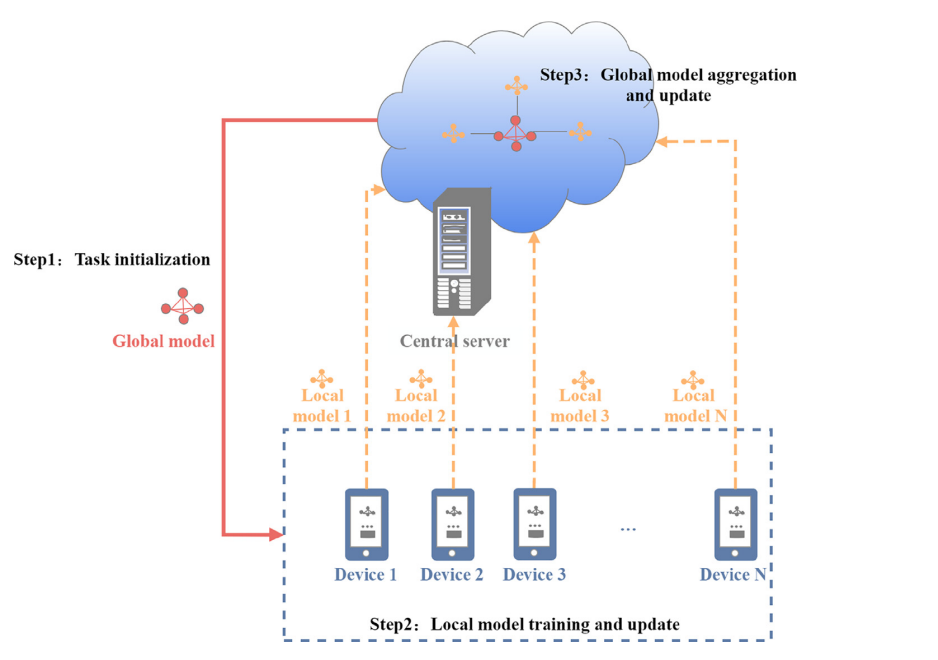
\includegraphics[scale=0.7]{images/chap1/federated_learning.png}%
	\caption{%
		یادگیری فدرال 
		\cite{ma2022state}%
		.
	}
	\label{federated_learning}
	\centering
\end{figure}

سرور در حقیقت نقش رهبری را ایفا می‌کند و با توجه به نوع داده‌ها، یک مدل شبکه عصبی%
\LTRfootnote{Neural Network}
ایجاد کرده و آن را به سمت کاربران ارسال می‌کند. در ادامه کاربران با توجه به داده‌های خود شبکه را آموزش می‌دهند و بعد از چند بار تکرار به صورت محلی، وزن‌های به‌روزرسانی شده را به سمت سرور بر می‌گردانند. همان‌طور که در شکل
\ref{federated_learning}
مشاهده می‌شود، داده‌ها همگی در سمت کاربران قرار گرفته‌اند و به سمت سرور ارسال نمی‌شوند. عدم اجبار در به اشتراک گذاشتن اطلاعات گره‌ها در یادگیری فدرال، کمک شایانی به حفظ حریم شخصی کاربران می‌کند
\cite{smith2017federated}.





% ابتدای فصل بهار سال 2017 محققین گوگل (Google) طی یک مطلب کوتاه در وبلاگ هوش مصنوعی، برای اولین بار موضـوع یادگیری فدرال را تحـت مطلبی با عنوان "یادگیری فدرال: یادگیری ماشین اشتـراکی، بدون آموزش متمرکز داده‌ها" مطرح نمودند. در این مطلب به طور کوتاه Google Keyboard یا به اختصار Gboard معرفی شد که با به کاری‌گیری یادگیری فدرال، لغت بعدی را پیش‌بینی و به کاربر توصیه می‌نمود. یادگیری فدرال در این کاربرد، نیاز به ارسال داده‌های کاربران به سمت سرور را حذف کرده است و به طور محلی مدل را به‌روزرسانی می‌کند.
%بنابراین، با بهره‌گیری از اطلاعات پنهان بسیار زیاد دستگاه‌ها در فرآیند مدل‌سازی، ضمن حفظ حریم شخصی سرویس‌گیرنده‌ها خدمات بهتری نسبت به قبل ارائه می‌گردد. در شکل نحوه استفاده از یادگیری فدرال در این برنامه به نمایش درآمده است.



\section{تاریخچه یادگیری فدرال}


در اوایل فصل بهار سال 2017، محققان گوگل
\lr{(Google)}
برای اولین بار موضوع یادگیری فدرال را در یک مطلب کوتاه در وبلاگ هوش مصنوعی خود معرفی کردند. این مطلب با عنوان «یادگیری فدرال: یادگیری ماشین اشتراکی، بدون نیاز به آموزش متمرکز داده‌ها» منتشر شد
\cite{mcmahan2017federated}.
در این نوشته، به طور مختصر از
\lr{Google Keyboard}
یا به اختصار
\lr{Gboard}
صحبت شد که با بهره‌گیری از یادگیری فدرال، قابلیت پیش‌بینی و پیشنهاد لغت بعدی به کاربر را دارد. با استفاده از یادگیری فدرال، دیگر نیازی به ارسال داده‌های کاربران به سرور نبود و مدل به ‌صورت محلی به‌روزرسانی می‌شد.

این روش با استفاده از اطلاعات فراوان ذخیره شده در دستگاه‌ها، خدمات بهتری را ارائه می‌دهد، بدون اینکه داده‌های حساس به سرور ارسال شوند و حریم شخصی کاربران به خطر بیفتد. در شکل
\ref{gboard}%
، نحوه استفاده از یادگیری فدرال در این برنامه به نمایش درآمده است.


%در ابتدای فصل بهار سال 2017 محققین گوگل
%\lr{(Google)}
%طی یک مطلب کوتاه در وبلاگ هوش مصنوعی، برای اولین بار موضـوع یادگیری فدرال را تحـت مطلبی با عنوان "یادگیری فدرال: یادگیری ماشین اشتـراکی، بدون آموزش متمرکز داده‌ها" مطرح نمودند
%\cite{mcmahan2017federated}%
%. در این مطلب به طور کوتاه
%\lr{Google Keyboard}
%یا به اختصار
%\lr{Gboard}
%معرفی شد که با به کاری‌گیری یادگیری فدرال، لغت بعدی را پیش‌بینی و به کاربر توصیه می‌نمود. یادگیری فدرال در این کاربرد، نیاز به ارسال داده‌های کاربران به سمت سرور را حذف کرده است و به طور محلی مدل را به‌روزرسانی می‌کند.
%بنابراین، با بهره‌گیری از اطلاعات پنهان بسیار زیاد دستگاه‌ها در فرآیند مدل‌سازی، ضمن حفظ حریم شخصی سرویس‌گیرنده‌ها خدمات بهتری نسبت به قبل ارائه می‌گردد.
%در شکل
%\ref{gboard}
%نحوه استفاده از یادگیری فدرال در این برنامه به نمایش درآمده است.

 \begin{figure}[t]
	\centering
	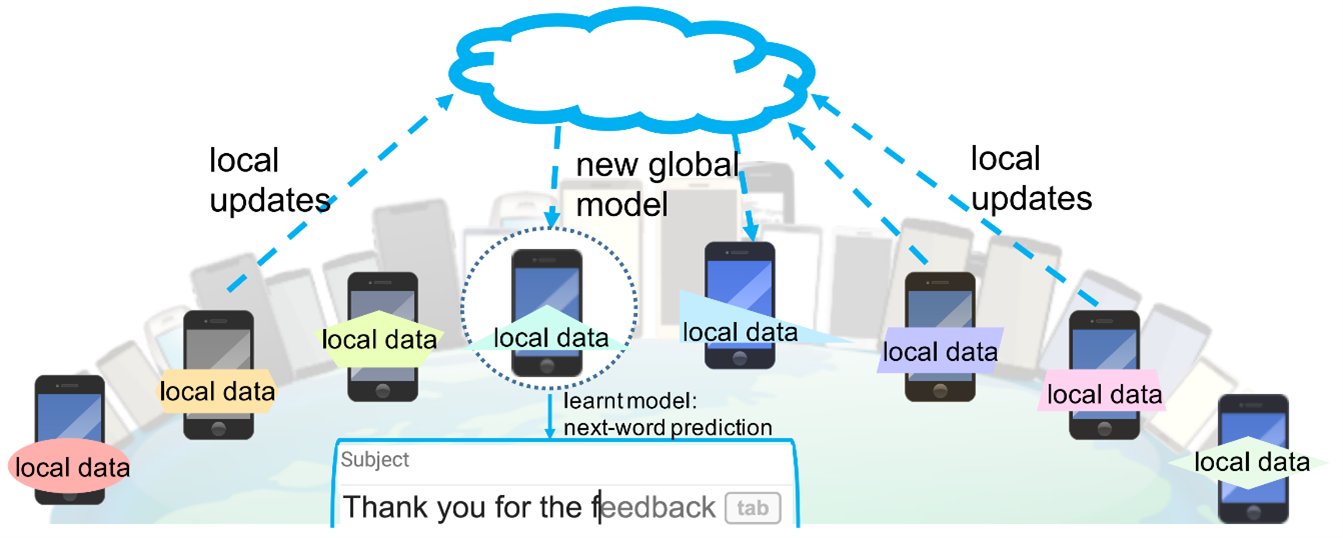
\includegraphics[scale=1]{images/chap1/gboard.png}%
	\caption{%
استفاده از یادگیری فدرال برای پیش‌بینی کلمه بعدی در
\lr{Gboard}
		\cite{li2020federated}%
		.
	}
	\label{gboard}
	\centering
\end{figure}



\section{کاربرد یادگیری فدرال}
ارتباطات نرم‌افزاری و سخت‌افزاری به معنای توانایی تبادل داده‌ها و هماهنگی عملکرد بین اجزای مختلف یک سیستم است، به طوری که این اجزا بتوانند به صورت یکپارچه و هماهنگ با یکدیگر کار کنند. فناوری مبتنی بر صنعت 4٫0%
\LTRfootnote{Industry 4.0}%
، این ارتباطات را در انواع سیستم‌ها به طور گسترده‌ای گسترش داده است. این هماهنگی بین نرم‌افزار و سخت‌افزار، به یک پدیده مهم در محیط‌های هوشمند و خودکار تبدیل شده است.

سامانه‌های متمرکز قبلی که تنها مسئول جمع‌آوری، پایش و کنترل شرایط به صورت محلی بودند، اکنون جای خود را به دستگاه‌های هوشمندی داده‌اند که قابلیت پردازش و برنامه‌ریزی داده‌ها را در سطح سیار و سیستمی دارند. علاوه بر این، گسترش ارتباطات مبتنی بر اینترنت، امکان انتقال و تبادل داده‌ها بین سیستم‌های مختلف را فراهم کرده است. این تحولات منجر به کاهش نیاز به تصمیم‌گیری متمرکز و توسعه سیستم‌های کنترل و پایش پیشرفته شده است. این ویژگی‌ها، همراه با حجم روزافزون داده‌ها، یادگیری فدرال را به یکی از بهترین روش‌ها برای توسعه سیستم‌های هوشمند تبدیل کرده است
\cite{mahtab2022algorithm}.
در ادامه، سه نمونه از کاربردهای یادگیری فدرال شرح داده خواهد شد.


\subsection{یادگیری فدرال در شهر هوشمند}
در یک شهر هوشمند%
\LTRfootnote{Smart City}%
، اطلاعات جمع‌آوری شده از حسگرهای مختلف مانند داده‌های ترافیک، مصرف انرژی، پسماند شهری و رویدادهای امنیتی، ارزش بالایی دارند و به عنوان منبعی کلیدی برای بهبود عملکرد شهر هوشمند و ارتقای کیفیت زندگی شهروندان محسوب می‌شوند. اما در کنار این مزایا، حفظ حریم شخصی و امنیت اطلاعات شهروندان نیز از اهمیت بالایی برخوردار است. یادگیری فدرال به عنوان یک رویکرد نوین که مبتنی بر حفظ حریم شخصی است، در اینجا به کار گرفته می‌شود.

در یک شهر هوشمند، سازمان‌های مختلف هر کدام اطلاعات خاص خود را دارند، اما این اطلاعات به طور متقابل بر یکدیگر تأثیر می‌گذارند و می‌توانند در مدیریت بهینه شهر نقش مهمی ایفا کنند. یادگیری فدرال با حفظ حریم شخصی کاربران، این امکان را فراهم می‌کند که سازمان‌ها بدون نیاز به اشتراک‌گذاری داده‌های حساس خود با یکدیگر، از داده‌های موجود بهره‌برداری کنند و مدل‌های هوش مصنوعی و الگوریتم‌های بهبود عملکرد شهر هوشمند را توسعه دهند. به عنوان مثال، با استفاده از یادگیری فدرال می‌توان بهبود مدیریت ترافیک، بهینه‌سازی مصرف انرژی، کاهش آلودگی هوا و افزایش امنیت شهری را تحقق بخشید، در حالی که حریم شخصی شهروندان به بهترین نحو ممکن حفظ می‌شود.


\subsection{یادگیری فدرال در بیمارستان}
در یک بیمارستان، اطلاعات پزشکی به شدت حساس و مهم هستند و باید به صورت محرمانه نگهداری شوند. با این حال، بهره‌برداری از این داده‌ها برای ارتقاء خدمات بهداشتی و درمانی بسیار ارزشمند است. در این شرایط، یادگیری فدرال می‌تواند نقش مهمی ایفا کند. با استفاده از روش‌های یادگیری فدرال، بیمارستان‌ها می‌توانند از داده‌های پزشکی بیماران خود برای توسعه مدل‌هایی استفاده کنند که به بهبود خدمات، ارتقاء روش‌های تشخیص و درمان بیماری‌ها و افزایش بهره‌وری پزشکان کمک می‌کنند، بدون اینکه نیاز باشد این داده‌ها به طور مستقیم به یک مرکز جمع‌آوری اطلاعات ارسال شوند.

برای مثال، با بهره‌گیری از یادگیری فدرال، مدل‌های هوش مصنوعی می‌توانند روی داده‌های محلی بیماران در هر بیمارستان آموزش داده شوند تا بیماری‌های مختلف را شناسایی و تشخیص دهند و اطلاعات مورد نیاز برای درمان‌های مؤثرتر را فراهم کنند، در حالی که اطلاعات حساس بیماران به طور کامل محافظت می‌شود. در شکل
\ref{hospital}
یک نمونه استفاده از یادگیری فدرال در بیمارستان‌ها به نمایش در آمده است.


\begin{figure}[t]
	\centering
	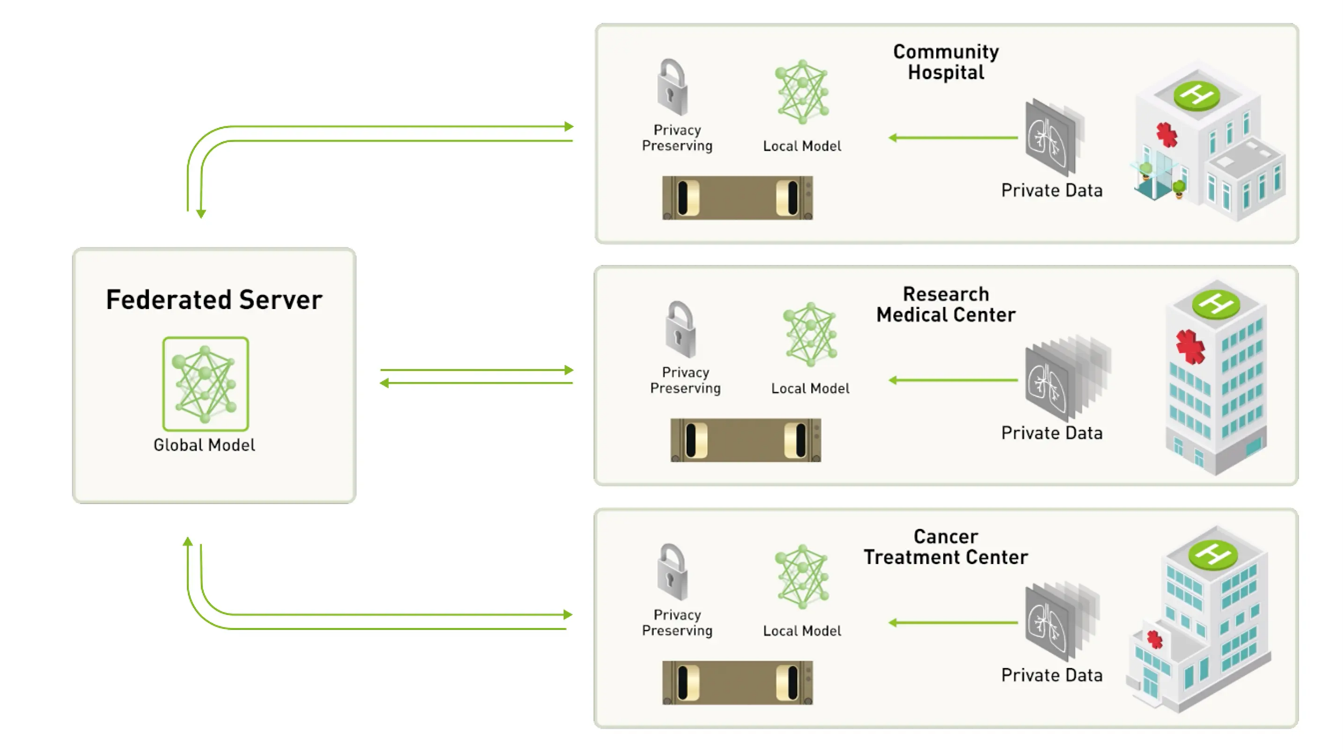
\includegraphics[scale=1]{images/chap1/hospital.png}%
	\caption{%
		یادگیری فدرال در بیمارستان
		\cite{rieke2019what}%
		.
	}
	\label{hospital}
	\centering
\end{figure}



\subsection{یادگیری فدرال در فروشگاه برنامه‌های کاربردی تلفن‌همراه}

یک فروشگاه برنامه‌های کاربردی%
\LTRfootnote{App Store}
تلفن‌همراه را در نظر بگیرید که به کاربران امکان دریافت و نصب برنامه‌های مختلف را می‌دهد. این فروشگاه می‌خواهد با استفاده از داده‌های کاربران خود، الگوریتمی توسعه دهد که بتواند به طور دقیق‌تری برنامه‌های مورد علاقه کاربران را پیشنهاد دهد. اگر این فروشگاه از روش‌های متمرکز استفاده کند، باید داده‌های حساس و شخصی کاربران را جمع‌آوری و تحلیل کند، که این موضوع می‌تواند نگرانی‌های جدی در مورد حریم خصوصی کاربران ایجاد کند و غیر عملی باشد.

با استفاده از یادگیری فدرال، این فروشگاه می‌تواند الگوریتم خود را بر روی داده‌های محلی هر کاربر اجرا کند. به این ترتیب، هیچ داده حساسی به یک مرکز جمع‌آوری داده‌ها ارسال نمی‌شود و حریم خصوصی کاربران حفظ می‌شود. به عنوان مثال، اگر یک کاربر به برنامه‌های موسیقی علاقه‌مند باشد، الگوریتم محلی در تلفن هوشمند او می‌تواند این الگو را شناسایی کند و پیشنهادات مربوط به برنامه‌های موسیقی را ارائه دهد، بدون این‌که نیاز به ارسال داده‌های شخصی و حساس او به سرور شرکت باشد.


\section{دید کلی از روند موضوع و بیان هدف پژوهش}
تکمیل این بخش پس از رسیدن به ساختار کلی پایان‌نامه (چون ممکنه در ادامه تغییر کنه)

چند جلمه کلیدی:

به دلیل پراکندگی همگرایی به کندی صورت می‌گیرد

روش جابجایی وزن‌ها بین کاربران نهایی در طول فرایند

چرا جابجایی تصادفی، جابجایی هوشمند بر اساس میزان شباهت

\section{مروی بر روند ارائه مطالب پایان‌نامه}
تست


% Chapter 2
\chapter{مفاهیم پایه در یادگیری فدرال}

\section{مقدمه}
توزیع داده‌ها بین کاربران در یادگیری فدرال ممکن است با چالش‌ها و مشکلات گوناگونی روبرو شود. یکی از مشکلات اساسی، اختلافات و ناسازگاری‌هایی است که ممکن است در فرآیند آموزش میان کاربران یا دستگاه‌های مختلف پدید آید. اگر این چالش‌ها پیش از آغاز فرآیند مدل‌سازی به درستی شناسایی نشده و راه‌حل‌های مناسبی برای آن‌ها اتخاذ نشود، مدل نهایی احتمالاً با مشکلاتی همچون کاهش دقت و عملکرد روبرو خواهد شد. این مسئله یکی از بزرگترین موانع در مسیر یادگیری فدرال است و نیازمند دقت و استفاده از روش‌های خلاقانه برای حل آن است.

در این فصل، ابتدا به بررسی چالش‌های موجود در یادگیری فدرال پرداخته خواهد شد و سپس دیدگاه‌های مقالات علمی در مورد هر یک از این چالش‌ها به صورت کلی بررسی می‌شود. در ادامه، بیان ریاضی یادگیری فدرال توضیح داده می‌شود و نهایتاً به رویکردهای کلی و اساسی برای حل این چالش‌ها اشاره خواهد شد.


\section{چالش‌های موجود در یادگیری فدرال و نگاه کلی مقالات به آن‌ها}
با وجود مزیت‌های بسیار زیاد نسبت به روش‌های سنتی یادگیری ماشین، یادگیری فدرال به دلیل ساختار شبکه یادگیری با چالش‌های گوناگونی روبرو است. چالش‌های اصلی یادگیری فدرال عبارتند از:


\subsection{تبادل داده}
تبادل داده بین سرور و کاربران به دلیل مشکلات پهنای باند و ارتباطات شبکه‌ای اصولا کار پر هزینه‌ای می‌باشد. یکی از دلایل اصلی پرهزینه بودن این ارتباطات، حجم بالای داده‌هایی است که باید بین دستگاه‌های کاربری و سرور منتقل شوند.
معمولاً مشکلات ارتباطی به انتقال‌های بسیار زیاد به‌روزرسانی‌های مدل بین گره‌های محاسباتی نسبت داده می‌شود. با افزایش تعداد پارامترها در مدل‌های پیشرفته، اندازه این مدل‌ها نیز به طور متناسب بزرگ می‌شود
\cite{wang2018atomo}.

از سوی دیگر، تعداد زیادی از دستگاه‌های کاربران نهایی در فرآیند آموزش مدل‌ها مشارکت دارند که این امر می‌تواند هزینه‌های ارتباطی را به طور قابل توجهی افزایش دهد. همچنین، به دلیل مشکلات ارتباطی، در بسیاری از مواقع همه دستگاه‌ها در هر چرخه از فرآیند آموزش شرکت نمی‌کنند که این مسئله نیز باعث افزایش هزینه‌ها و پیچیدگی‌های مرتبط با انتقال داده‌ها می‌شود.


\subsection{
	ناهمگنی‌های سیستمی
\LTRfootnote{Systems Heterogeneity}
}
در دنیای یادگیری فدرال، دستگاه‌ها از نظر حافظه، توان محاسباتی و ارتباطات بسیار با یکدیگر متفاوت هستند. این تفاوت‌ها ممکن است از اختلافاتی مانند تفاوت در پردازنده، نوع حافظه، نوع اتصال شبکه و نیاز به انرژی ناشی شود. محدودیت‌های موجود در شبکه و سیستمی می‌توانند باعث ایجاد وضعیت‌هایی شوند که برخی از دستگاه‌ها در یک زمان معین در دسترس نباشند. برای مثال، اگر تعداد زیادی دستگاه همزمان درخواست ارسال داشته باشند، ممکن است برخی از آن‌ها به دلیل پهنای باند محدود یا محدودیت‌های سخت‌افزاری، قادر به ارسال درخواست نشوند. همچنین، ممکن است یک دستگاه فعال، به دلیل مشکلاتی مانند اختلالات در شبکه یا مصرف اضافی انرژی، از فرآیند یادگیری خارج شود.

این تفاوت‌های سیستمی، یکی از چالش‌های یادگیری فدرال محسوب می‌شوند و می‌توانند باعث افزایش تأخیر و ایجاد اشکالات در سیستم شوند. بنابراین، برای رفع این مشکلات، روش‌های یادگیری فدرال باید توانایی پیش‌بینی دقیق تعداد دستگاه‌هایی که در هر فرآیند شرکت می‌کنند را داشته باشند. همچنین، باید بتوانند در برابر دستگاه‌هایی که در حین عملیات دچار مشکل شده و از دسترس خارج می‌شوند، مقاومتی مناسب داشته باشند
\cite{li2020federated}.


\subsection{
	ناهمگنی‌های آماری
\LTRfootnote{Statistical Heterogeneity}
}
روش‌های مختلفی برای تولید و جمع‌آوری داده‌ها بین دستگاه‌ها وجود دارد. این داده‌ها معمولاً به صورت مستقل از هم تولید نمی‌شوند و بین آن‌ها ارتباطات و پیوندهایی وجود دارد. چنین الگویی از تولید داده با فرضیات استقلال و توزیع یکنواخت داده‌ها%
\LTRfootnote{Independent and Identically Distributed}
\lr{(IID)}
در مسائل بهینه‌سازی در تضاد است، که منجر به پیچیدگی‌هایی در فرآیند مدل‌سازی، تحلیل نظری و ارزیابی عملکرد می‌شود. بنابراین، با وجود هدف نهایی که یادگیری یک مدل جامع و یکپارچه است، روش‌های جایگزین مانند یادگیری چندوظیفه‌ای%
\LTRfootnote{Multi-Tasking}
و فرایادگیری%
\LTRfootnote{Meta Learning}
به عنوان راه‌حل‌های ممکن مطرح شده‌اند
\cite{li2020federated}.



\subsection{حریم شخصی}
یکی از چالش‌های اساسی در یادگیری فدرال، حفظ حریم شخصی است که در این روش، داده‌های حساس و شخصی در اختیار بخش‌های مختلفی از شبکه قرار می‌گیرند. در این روش، دستگاه‌های محلی اطلاعاتی از کاربران جمع‌آوری و به سرور ارسال می‌کنند تا مدل‌های یادگیری مشترک را به‌روزرسانی کنند. این ارتباطات می‌توانند حاوی اطلاعات حساسی باشند که می‌توانند به راحتی به شناسایی فرد یا فرآیندهای حیاتی او منجر شوند.

یکی از مشکلات اساسی در اینجا این است که حتی با استفاده از روش‌های رمزنگاری و حفظ امنیت، اطلاعات معینی همچنان ممکن است به سرور ارسال شود که احتمالاً می‌تواند حریم شخصی را نقض کند. به‌طور خاص، اگر داده‌های حساس بدون رمزنگاری به سرور ارسال شوند یا اگر حتی اطلاعاتی که قابلیت شناسایی فرد را دارند به صورت رمزگذاری نشده ارسال شوند، حریم شخصی کاربران مورد تهدید قرار می‌گیرد.


\section{نگاه مقالات مرتبط به چالش‌های موجود}

\subsection{تبادل داده}
با استفاده از فشرده‌سازی داده‌ها، می‌توان هزینه‌های ارتباطی را به طور قابل توجهی کاهش داد. دو روش جهت مدیریت هزینه‌های بالای ارتباطات در فرایند یادگیری فدرال مورد بررسی قرار گرفته است. این روش‌ها به فشرده‌سازی داده‌هایی که از دستگاه‌های کاربری به سرور مرکزی ارسال می‌شوند متمرکز شده‌اند. این فشرده‌سازی اطلاعات ارسالی به گونه‌ای است که حجم داده‌های ارسالی کم شده و در نتیجه، هزینه‌های مربوط به ارتباطات نیز کاهش یابد
\cite{konevcny2016federated}.

در روشی به نام
\lr{PCFL}%
\LTRfootnote{Privacy Communication efficient Federated Learning}
که یک رویکرد حفظ حریم خصوصی و البته بسیار کارآمد از نظر ارتباطی می‌باشد، شامل سه جزء کلیدی است که به ترتیب از فشرده‌سازی دوطرفه، فشرده‌سازی مکانی گرادیان‌ها و یک پروتکل حفظ حریم خصوصی که خود از تقسیم راز%
\LTRfootnote{Secret Sharing}
 و رمزنگاری همگام%
 \LTRfootnote{Homomorphic Encryption}
  برای محافظت از حریم خصوصی داده‌ها استفاده می‌کند، بهره گرفته است
  \cite{fang2021privacy}.


\subsection{ناهمگنی سیستمی و آماری}
برای مقابله با ناهمگنی سیستمی و آماری، روش‌هایی مانند تعادل در به‌روزرسانی مدل مطرح شده است. در این روش، وزن‌دهی به نمونه‌ها بر اساس میزان نیاز به آموزش در هر دستگاه صورت می‌گیرد. این کار باعث می‌شود که دستگاه‌های با حجم داده کمتر، وزن بیشتری در به‌روزرسانی مدل داشته باشند
\cite{konevcny2015federated}.
در رویکرد دیگری به نام یادگیری فعال، دستگاه‌هایی که داده‌های خود را به سرور ارسال می‌کنند، فعالیت خود را به نحوی تنظیم می‌کنند که مدل از داده‌های مهم‌تر و کمتر دیده شده بیشتر یاد می‌گیرد. این روش می‌تواند به تعادل در آموزش مدل کمک کند و از ناهمگنی سیستمی جلوگیری کند
\cite{konevcny2016federated}.

یک روش دیگر برای حل مشکل ناهمگنی سیستمی و آماری در یادگیری فدرال استفاده از رویکرد ترکیبی یا ترکیب روش‌های یادگیری محلی است. در این رویکرد، به جای استفاده از یک الگوریتم یادگیری مشترک برای تمام دستگاه‌ها، از چندین الگوریتم یادگیری محلی با تنوع مدل‌ها و تنظیمات مختلف استفاده می‌شود. سپس، اطلاعات مدل‌های محلی روی سرور یا گره مرکزی جمع‌آوری می‌شود و با استفاده از ترکیب این اطلاعات، یک مدل یادگیری مشترک بروزرسانی خواهد شد
\cite{konevcny2015federated}.


\subsection{حریم شخصی}
در روش حفظ حریم خصوصی تفاضلی%
\LTRfootnote{Differential Privacy}
با افزودن نویز به نتایج محاسبات یا به داده‌های ورودی، اطمینان حاصل می‌کند که حضور یا عدم حضور یک نمونه داده خاص در مجموعه داده‌ها، تأثیر قابل توجهی بر خروجی محاسبات نداشته باشد. این روش به ویژه برای حفظ حریم خصوصی در یادگیری فدرال مفید است زیرا از افشای اطلاعات حساس از طریق پارامترهای مدل جلوگیری می‌کند
\cite{hasan2023security}.

رویکرد رمزنگاری همگام امکان محاسبه روی داده‌های رمزنگاری شده را بدون نیاز به رمزگشایی آن‌ها فراهم می‌کند. این تکنیک به ویژه در یادگیری فدرال برای حفظ حریم خصوصی داده‌ها در حین انجام محاسبات مفید است زیرا نیاز به تغییر ماهیت داده نبوده و چون جابجایی در یادگیری فدرال بسیار زیاد رخ می‌دهد، این روش بسیار کارا خواهد بود
\cite{yin2021comprehensive}.



\section{بیان ریاضی یادگیری فدرال}
برای ورود به مباحث ریاضی پایه در یادگیری فدرال، ابتدا باید به تعریف دقیق مسئله بهینه‌سازی مرکزی بپردازیم که در این حوزه مطرح می‌شود. در یادگیری فدرال، هدف اصلی یافتن مجموعه‌ای از پارامترهای مدل است که عملکرد کلی مدل را بر روی داده‌های توزیع‌شده بین تعداد زیادی دستگاه بهینه کند. هر دستگاه دارای داده‌های محلی است و یک تابع هزینه محلی بر اساس این داده‌ها برای آن دستگاه تعریف می‌شود. مسئله بهینه‌سازی کلی در یادگیری فدرال به دنبال کمینه کردن مجموع وزنی این توابع هزینه محلی است تا یک مدل جامع و یکپارچه حاصل شود.

ما یک طرح به‌روزرسانی همزمان را فرض می‌کنیم که به صورت دوره‌های ارتباطی پیش می‌رود. یک مجموعه ثابت از
$K$
مشتری وجود دارد که هر کدام یک مجموعه داده محلی ثابت دارند. در ابتدای هر دوره، یک کسر تصادفی
$C$
از مشتری‌ها انتخاب می‌شوند و سرور وضعیت فعلی پارامترهای مدل جهانی را به هر یک از این مشتری‌ها ارسال می‌کند. هر مشتری انتخاب ‌شده سپس بر اساس وضعیت جهانی و مجموعه داده محلی خود محاسبات محلی را انجام می‌دهد و یک به‌روزرسانی به سرور ارسال می‌کند. سپس سرور این به‌روزرسانی‌ها را به وضعیت جهانی خود اعمال می‌کند و این فرآیند تکرار می‌شود
\cite{mcmahan2017communication}.

در حالی که ما بر اهداف شبکه عصبی غیرمحدب
\LTRfootnote{Non-Convex}
تمرکز داریم، الگوریتمی که بررسی می‌کنیم قابل اعمال به هر هدف مجموع-متناهی
\LTRfootnote{Finite-Sum}
به صورت زیر است.
\begin{equation}
\min _{w \in \mathbb{R}^d} f(w) \quad \text { where } \quad f(w) \stackrel{\text { def }}{=} \frac{1}{n} \sum_{i=1}^n f_i(w)
\label{eq_base}
\end{equation}
برای یک مسئله یادگیری ماشین، معمولاً
$f_i(w)=\ell\left(x_i, y_i ; w\right)$
در نظر گرفته می‌شود، به این معنی که این تابع نشان‌دهنده‌ی خطای پیش‌بینی بر روی نمونه
$(x_i, y_i)$
با استفاده از پارامترهای مدل
$w$
است. فرض می‌کنیم که داده‌ها بین
$K$
مشتری تقسیم شده‌اند، که در آن
$\mathcal{P}_k$
مجموعه‌ای از نقاط داده مربوط به مشتری
$k$
است و
$n_k=\left|\mathcal{P}_k\right|$
تعداد این نقاط داده را نشان می‌دهد. بنابراین، می‌توانیم فرمول
\ref{eq_base}
را به صورت زیر بازنویسی کنیم:
\begin{equation}
f(w)=\sum_{k=1}^K \frac{n_k}{n} F_k(w) \quad \text { where } \quad F_k(w)=\frac{1}{n_k} \sum_{i \in \mathcal{P}_k} f_i(w)
\end{equation}

اگر مجموعه
$\mathcal{P}_k$
با توزیع یکنواخت تصادفی از مثال‌های آموزشی بین مشتری‌ها تشکیل شده باشد، در آن صورت
$\mathbb{E}_{\mathcal{P}_k}\left[F_k(w)\right]=f(w)$ 
خواهد بود، که در اینجا امید ریاضی بر روی مجموعه مثال‌های اختصاص داده شده به یک مشتری ثابت گرفته می‌شود. این همان فرض
\lr{IID}
(استقلال و توزیع یکسان)
است که عموماً توسط الگوریتم‌های بهینه‌سازی توزیع‌شده استفاده می‌شود، در این‌جا ما حالتی را که این فرض برقرار نیست (یعنی
$F_k$
می‌تواند تقریباً به هر میزانی از
$f$
فاصله داشته باشد) به عنوان حالت
\lr{Non-IID}
(غیرمستقل و غیریکنواخت)
می‌شناسیم
\cite{mcmahan2017communication}.


\section{رویکردهای کلی و پایه‌ای در حل چالش‌ها}
روش‌های بهینه‌سازی توزیع‌شده معمولاً برای حل مسائل بهینه‌سازی در سیستم‌هایی با شبکه‌های محاسباتی بزرگ و توزیع‌شده استفاده می‌شوند. این روش‌ها بر مبنای تقسیم مسئله بهینه‌سازی به زیرمسائل کوچک‌تر و حل آن‌ها در گره‌های مختلف شبکه استوارند. در این روش‌ها، اغلب فرض می‌شود که داده‌ها به صورت همگن و یکپارچه در سراسر شبکه توزیع شده‌اند و گره‌ها می‌توانند به راحتی با یکدیگر ارتباط برقرار کنند.

فرضیات مطرح شده در یادگیری فدرال به ندرت برقرار است، زیرا در یادگیری فدرال داده‌ها به صورت محلی و ناهمگن در دستگاه‌های مختلف قرار دارند و ارتباطات بین دستگاه‌ها ممکن است محدود و نامنظم باشد. بنابراین روش‌ها و رویکردهای لازم جهت حل این چالش‌ها متفاوت از مسائل بهینه‌سازی توزیع شده هستند. حال سعی می‌کنیم دو رویکرد پایه‌ای برای مسائل یادگیری فدرال را مطرح نماییم.

\subsection{به‌روزرسانی محلی و میانگین‌گیری در سرور}
یکی از روش‌های اصلی و پرکاربرد در یادگیری فدرال روش میانگین‌گیری فدرال%
\LTRfootnote{Federated Averaging}
\lr{(FedAvg)}
است که توسط محققان گوگل در سال 2017 معرفی شد. این الگوریتم به منظور بهینه‌سازی مدل‌های یادگیری ماشین در یک محیط توزیع‌شده طراحی شده است، جایی که داده‌ها به صورت محلی در دستگاه‌های کاربران باقی می‌مانند و تنها به‌روزرسانی‌های مدل به اشتراک گذاشته می‌شوند. رویکرد اصلی
\lr{FedAvg}
بر مبنای ترکیب به‌روزرسانی‌های محلی از دستگاه‌های مختلف به یک مدل جهانی استوار است.

یکی از مزایای اصلی
\lr{FedAvg}
این است که به طور موثری با چالش ناهمگنی داده‌ها مقابله می‌کند. در یادگیری فدرال، داده‌های موجود در دستگاه‌های مختلف ممکن است توزیع‌های متفاوتی داشته باشند. این ناهمگنی می‌تواند به دلیل تفاوت در رفتار کاربران یا حتی محیط‌های مختلف جمع‌آوری داده باشد. میانگین‌گیری وزنی در
\lr{FedAvg}
به مدل کمک می‌کند تا به‌روزرسانی‌های مختلف را به گونه‌ای ترکیب کند که این ناهمگنی‌ها را در نظر بگیرد. به عبارت دیگر، اگر یک دستگاه داده‌های بیشتری داشته باشد، تأثیر بیشتری بر مدل نهایی خواهد داشت. این رویکرد باعث می‌شود که مدل فدرال به تعادل بهتری در یادگیری از داده‌های ناهمگن برسد و کارایی بالاتری داشته باشد. این ویژگی به خصوص در کاربردهایی که کاربران متنوع و داده‌های متنوعی دارند، بسیار مفید است و می‌تواند به بهبود عملکرد مدل در شرایط واقعی کمک کند.

علاوه بر این،
\lr{FedAvg}
به کاهش نیاز به ارتباطات مکرر بین دستگاه‌ها و سرور مرکزی کمک می‌کند. در بسیاری از روش‌های بهینه‌سازی توزیع‌شده، نیاز است که دستگاه‌ها به طور مکرر با سرور مرکزی ارتباط برقرار کنند تا به‌روزرسانی‌های خود را ارسال کنند. اما در
\lr{FedAvg}
دستگاه‌ها می‌توانند چندین مرحله از بهینه‌سازی را به صورت محلی انجام دهند و سپس تنها به‌روزرسانی نهایی را ارسال کنند. این کاهش در نیاز به ارتباطات نه تنها باعث کاهش پهنای باند مورد نیاز می‌شود، بلکه به حفظ حریم خصوصی کاربران نیز کمک می‌کند، زیرا داده‌ها هرگز از دستگاه‌های محلی خارج نمی‌شوند. بررسی‌ها نشان داده‌اند که متناسب با اندازه داده‌ها پس از رسیدن به تعداد معینی از گره‌ها، اضافه کردن گره‌های بیشتر تأثیری در کاهش هزینه‌های ارتباطی نخواهد داشت. در چنین شرایطی، تمرکز بر افزایش توان محاسباتی محلی یا تعداد مراحل آموزش محلی می‌تواند موجب تسریع فرایند آموزش شود
\cite{mcmahan2017communication}.

موفقیت‌های اخیر در کاربردهای یادگیری عمیق تقریباً به‌طور انحصاری به استفاده از انواع الگوریتم نزول گرادیان تصادفی%
\LTRfootnote{Stochastic Gradient Descent}
\lr{(SGD)}
برای بهینه‌سازی متکی بوده‌اند. در واقع، بسیاری از پیشرفت‌ها به تنظیم مدل و بهینه‌سازی تابع خطا با روش‌های ساده گرادیان مربوط می‌شود. بنابراین، طبیعی است که ما الگوریتم‌های بهینه‌سازی فدرال را با شروع از
\lr{SGD}
بسازیم.

الگوریتم
\lr{SGD}
می‌تواند به سادگی در بهینه‌سازی فدرال استفاده شود، به این صورت که در هر دور ارتباط، گرادیان‌ها بر اساس داده‌های یک مشتری تصادفی انتخاب شده، محاسبه ‌شوند. این رویکرد از نظر محاسباتی کارآمد است، اما نیازمند تعداد بسیار زیادی از دورهای آموزش برای تولید مدل‌های خوب است.
برای مثال حتی با استفاده از رویکرد پیشرفته‌ای مانند نرمال‌سازی دسته‌ای%
\LTRfootnote{Batch Normalization}%
، برای آموزش دیتاست معروف
\lr{MNIST}
(دیتاستی جهت دسته‌بندی اعداد دستنویس بین صفر تا نه)
با دسته‌های کوچکی به اندازه 60 به 50000 دور آموزش جهت رسیدن به مدل مطلوب نیاز می‌باشد
\cite{ioffe2015batch}.

در تنظیمات فدرال، مشارکت تعداد زیادتری از مشتریان هزینه‌ای آنچنان بیشتری در زمان واقعی ندارد زیرا همه کاربران می‌توانند به صورت همزمان اقدام به آموزش مدل محلی کنند، بنابراین برای خط مبنای خود از
\lr{SGD}
همزمان با دسته‌های بزرگ استفاده می‌کنیم. برای اعمال این رویکرد در تنظیمات فدرال، ما در هر دور یک کسر
$C$
از مشتریان را انتخاب می‌کنیم و گرادیان خطا روی تمام داده‌های نگهداری شده توسط این مشتریان را محاسبه می‌کنیم. بنابراین
$C$
اندازه دسته‌ کلی را کنترل می‌کند، به‌طوری که
$C = 1$
معادل با نزول گرادیان یک دسته کامل است. حال این الگوریتم خط مبنا را
\lr{FederatedSGD}
یا
\lr{FedSGD}
می‌نامیم.

یک پیاده‌سازی معمول از
\lr{FedSGD}
با
$C = 1$
و نرخ یادگیری ثابت
$\eta$
به این صورت است که هر گره
$k$%
، گرادیان
$g_k=\nabla F_k\left(w_t\right)$
که میانگین گرادیان روی داده‌های محلی در مدل فعلی
$w_t$
است را محاسبه می‌کند و سرور مرکزی این گرادیان‌ها را جمع‌آوری کرده و به‌روزرسانی
$w_{t+1} \leftarrow w_t-\eta \sum_{k=1}^K \frac{n_k}{n} g_k$
را انجام می‌دهد، در حالی که
$\sum_{k=1}^K \frac{n_k}{n} g_k=\nabla f\left(w_t\right)$
خواهد بود. یک به‌روزرسانی معادل به این صورت است که برای هر گره عبارت
$\forall k, w_{t+1}^k \leftarrow w_t-\eta g_k$
محاسبه و سپس
$w_{t+1} \leftarrow \sum_{k=1}^K \frac{n_k}{n} w_{t+1}^k$
انجام شود.

در نتیجه، هر گره به صورت محلی یک گام گرادیان نزولی را روی مدل فعلی با استفاده از داده‌های محلی خود طی می‌کند و سپس سرور میانگین وزنی مدل‌های حاصل را محاسبه می‌کند. وقتی که الگوریتم به این صورت نوشته شود، می‌توانیم با تکرار به‌روزرسانی محلی
$w^k \leftarrow w^k-\eta \nabla F_k\left(w^k\right)$%
، چندین بار قبل از مرحله میانگین‌گیری، محاسبات بیشتری به هر گره اضافه کنیم. در نهایت این رویکرد جدید را
\lr{FederatedAveraging}
\lr{(FedAvg)}
می‌نامیم.

میزان محاسبات توسط سه پارامتر کلیدی کنترل می‌شود:
$C$%
، کسر گره‌هایی که در هر مرحله محاسبات انجام می‌دهند؛
$E$%
، تعداد مراحل آموزشی که هر گره در هر دور روی مجموعه داده محلی خود انجام می‌دهد؛ و
$B$%
، اندازه دسته محلی که برای به‌روزرسانی‌های هر گره استفاده می‌شود. در اینجا
$B = \infty$
را می‌نویسیم تا نشان دهیم که کل مجموعه داده محلی به عنوان یک دسته واحد در نظر گرفته می‌شود. بنابراین، به عنوان یک نمونه از این الگوریتم گسترده شده جدید، می‌توانیم
$B = \infty$
و
$E = 1$
را انتخاب کنیم که در این حالت دقیقاً با
\lr{FedSGD}
برابر خواهد شد. همچنین برای یک گره با
$n_k$
نمونه محلی، تعداد به‌روزرسانی‌های محلی در هر دور با
$u_k=E \frac{n_k}{B}$
نمایش داده می‌شود
\cite{mcmahan2017communication}.



\subsection{
بهینه‌سازی
\lr{\texttt{\fontspec{Times New Roman} FedProx}}
}
روش
\lr{FedProx}
به بررسی چالش‌های یادگیری فدرال در بسترهای ناهمگن می‌پردازد. این روش با ایجاد تغییرات جزئی در روش موجود
\lr{FedAvg}%
، به بهبود پایداری و دقت در شبکه‌های ناهمگن کمک می‌کند. این تغییرات شامل اضافه کردن یک عبارت نزدیک مبدا%
\LTRfootnote{Proximal Term}
به تابع هدف است که به صورت اصولی به سرور کمک می‌کند تا ناهمگنی را مدیریت کند.

فرمول هدف
\lr{FedProx}
به صورت زیر تعریف می‌شود:
\begin{equation}
\min_{w} f(w) = \min_{w} \sum_{k=1}^{K} \frac{n_k}{n} \left( F_k(w) + \frac{\mu}{2} \|w^t - w_k^t\|^2 \right)
\label{eq_FedProx}
\end{equation}

در فرمول
\ref{eq_FedProx}
بخش
$\frac{\mu}{2} \|w^t - w_k^t\|^2$%
، همان عبارت نزدیک مبدا است که به تابع هدف اضافه شده است. همچنین
$\mu$%
، یک پارامتر تنظیم برای این عبارت به حساب می‌آید و در نهایت
$w_k^t$
وزن‌های مدل محلی دستگاه
$k$
در تکرار
$t$
است.

حال با توجه به فرمول
\ref{eq_FedProx}%
، به‌روزرسانی وزن‌ها به شکل زیر تغییر پیدا خواهد کرد و بخش
$\mu (w^t - w_k^t)$%
، گرادیان عبارت نزدیک مبدا است.
\begin{equation*}
w^{t+1} = w^t - \eta (\nabla F_k(w^t) + \mu (w^t - w_k^t))
\end{equation*}

بنابراین، به‌روزرسانی‌های محلی در هر گام با به‌روزرسانی سراسری مرحله قبل مرتبط هستند. عبارت نزدیک مبدا به عنوان یک مکانیزم منظم‌کننده%
\LTRfootnote{Regularization}
عمل می‌کند که تفاوت‌های بین وزن‌های جهانی
$w$
و وزن‌های محلی
$w_k^t$
را کاهش می‌دهد. این ترم به کاهش تاثیرات منفی ناهمگنی سیستم‌ها و داده‌ها کمک می‌کند و باعث پایداری بیشتر در فرآیند همگرایی می‌شود
\cite{li2020federatedheteroneneous}.


% Chapter 3
\chapter{بررسی پیشینه روش‌های حل مشکل ناهمگنی آماری}

\section{مقدمه}
همان‌طور که در فصل گذشته اشاره شد، یکی از مهم‌ترین مشکلات در حوزه یادگیری فدرال، مسئله داده‌های غیرمستقل و غیریکنواخت
\lr{(non-IID)}
است که منجر به بروز چالش‌ها و ناهمگنی‌های آماری می‌شود. این مشکل باعث می‌شود که مدل‌های یادگیری نتوانند به خوبی از داده‌های توزیع‌شده استفاده کنند و کارایی مطلوبی داشته باشند. به دلیل اهمیت بالای این موضوع، محققان بسیاری تلاش‌های گسترده‌ای برای حل این مشکل انجام داده‌اند.

مبحث اصلی این پایان‌نامه نیز به طور دقیق به همین مسئله اشاره دارد و به دنبال یافتن راه‌حلی مؤثر برای مقابله با داده‌های
\lr{non-IID}
است. در ادامه، به صورت خلاصه به بررسی راه‌حل‌هایی که تاکنون برای حل این مشکل مطرح شده‌اند، خواهیم پرداخت تا تصویر جامعی از تلاش‌های انجام شده در این زمینه ارائه دهیم. همچنین باید توجه داشت که هر یک از این راه‌حل‌ها نقاط قوت و ضعف خاص خود را دارند و بسته به شرایط و نوع داده‌ها، می‌توانند نتایج متفاوتی را به همراه داشته باشند. بررسی دقیق این راه‌حل‌ها و ارزیابی کارایی آن‌ها می‌تواند به بهبود سیستم‌های یادگیری فدرال و غلبه بر مشکلات مرتبط با داده‌های غیرمستقل و غیر یکنواخت کمک شایانی کند.

\section{نگرش برپایه داده}
\subsection{اشتراک‌گذاری داده}
مشکل اصلی الگوریتم
\lr{FedAvg}
در مواجهه با داده‌های غیرمستقل و غیریکنواخت، تفاوت وزن‌های اولیه در شروع فرآیند آموزش است. این تفاوت‌ها می‌توانند باعث شوند که مدل‌های محلی در هر گره به طور قابل توجهی متفاوت از یکدیگر باشند، که در نتیجه منجر به مشکلات همگرایی و کاهش کارایی مدل نهایی می‌شود.

برای رفع این مشکل، روشی پیشنهاد شده است که در آن ابتدا سرور مرکزی مقدار کمی از داده‌ها را به صورت محلی آموزش می‌دهد. در این مرحله، سرور مرکزی با استفاده از این داده‌ها، یک مدل اولیه را آموزش داده و وزن‌های اولیه آن را تنظیم می‌کند. سپس، این وزن‌های اولیه به همراه داده‌های آموزش دیده شده به تمامی کاربران ارسال می‌شود. این اقدام باعث می‌شود که تمام کاربران در ابتدای فرآیند آموزش با مجموعه‌ای از داده‌های مشترک و وزن‌های اولیه مشابه روبه‌رو شوند.

نقطه قوت این روش در این است که به دلیل انجام این عملیات تنها در آغاز فرآیند آموزش، هزینه زیادی به شبکه تحمیل نمی‌شود. در واقع، انتقال داده‌ها و وزن‌ها فقط در ابتدا انجام شده و پس از آن کاربران به صورت مستقل به آموزش مدل‌های محلی خود ادامه می‌دهند. این اقدام منجر به کاهش اختلافات ناشی از ناهمگنی داده‌ها شده و فرآیند همگرایی مدل نهایی سریع‌تر و با دقت بیشتری انجام می‌شود
\cite{zhao2018federated}.

در شکل
\ref{share_data}%
، نحوه اجرای این روش و مراحل مختلف آن به تصویر کشیده شده است. این تصویر نشان می‌دهد که چگونه سرور مرکزی ابتدا داده‌های کمی را آموزش می‌دهد، وزن‌های اولیه را تنظیم می‌کند و سپس این وزن‌ها و داده‌ها را به کاربران ارسال می‌کند تا فرآیند آموزش محلی با یک نقطه شروع مشترک برای همه کاربران آغاز شود.

یکی دیگر از روش‌های مطرح شده در زمینه یادگیری فدرال به این صورت است که کاربران بتوانند نتایج آموزش تعدادی داده اشتراکی را با یکدیگر به اشتراک بگذارند و از نتایج دیگر کاربران بر روی این داده‌های اشتراکی مطلع شوند. در این روش، کاربران نتایج به‌دست آمده از آموزش داده‌های مشترک را با هم مبادله می‌کنند، که این کار منجر به بهبود عملکرد مدل‌های محلی و در نهایت مدل سراسری می‌شود
\cite{collins2021exploiting}.

براساس بررسی‌های انجام شده، مثلاً در مجموعه داده
\lr{CIFAR-10}،
اگر حدود 5 درصد از داده‌ها به صورت اشتراکی در اختیار کاربران قرار گیرد، دقت مدل تا حدود 30 درصد افزایش خواهد یافت. این افزایش دقت به دلیل همگرایی بهتر مدل‌ها و کاهش تفاوت‌های آماری بین داده‌های محلی است. به عبارتی دیگر، این روش کمک می‌کند که مدل‌ها با یکدیگر هماهنگ‌تر شوند و نتایج دقیق‌تری ارائه دهند.

با این حال، باید توجه داشت که اشتراک‌گذاری داده‌ها بین کاربران می‌تواند مسائل حریم شخصی را به همراه داشته باشد. به عبارت دیگر، هنگامی که داده‌های اشتراکی بین کاربران مبادله می‌شود، احتمال نقض حریم شخصی کاربران افزایش می‌یابد. بنابراین، هنگام پیاده‌سازی این روش، ضروری است که اقدامات لازم برای حفظ حریم شخصی کاربران به طور جدی مد نظر قرار گیرد. این اقدامات می‌تواند شامل استفاده از تکنیک‌های رمزنگاری، ناشناس‌سازی داده‌ها، یا روش‌های دیگر برای محافظت از اطلاعات حساس کاربران باشد
\cite{ma2022state}.

در نهایت، روش به اشتراک‌گذاری داده‌ها بین کاربران، اگرچه می‌تواند به بهبود دقت و کارایی مدل‌ها کمک کند، اما نیازمند دقت و توجه ویژه‌ای به مسائل حریم شخصی است. پژوهشگران و توسعه‌دهندگان باید با در نظر گرفتن این چالش‌ها، راهکارهایی را برای حفظ امنیت و حریم شخصی کاربران در هنگام اجرای این روش‌ها ارائه دهند.

 \begin{figure}[t]
	\centering
	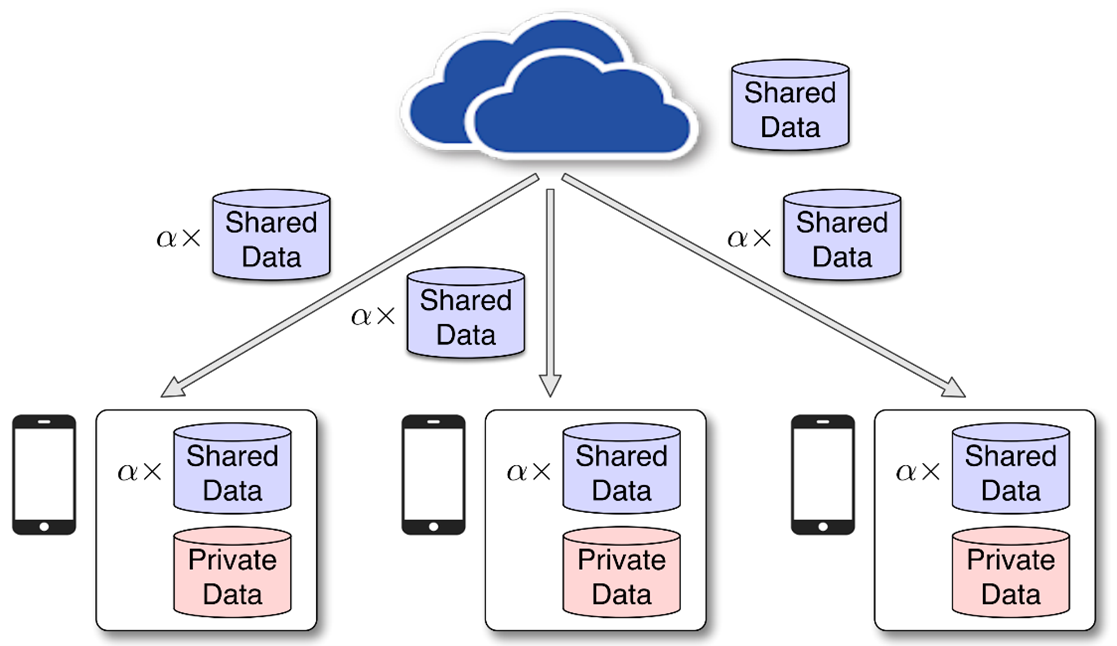
\includegraphics[scale=0.9]{images/chap3/share_data.png}%
	\caption{%
		نمایش نحوه به اشتراک‌ گذاری داده
		\cite{zhao2018federated}%
		.
	}
	\label{share_data}
	\centering
\end{figure}


\subsection{
	بهبود داده%
\protect
\LTRfootnote{Data Enhancement}
}
ابتدا، کاربران تعدادی از داده‌های خود را به سمت سرور ارسال می‌کنند. سرور، با استفاده از داده‌های دریافتی، یک مدل شبکه مولد رقابتی%
\LTRfootnote{Generative Adversarial Network (GAN)}
ایجاد می‌کند و این مدل را برای تمامی کاربران ارسال می‌نماید. کاربران با استفاده از این شبکه مولد رقابتی و با توجه به داده‌های خود، تعدادی داده جدید تولید کرده و در مراحل بعدی آموزش از این داده‌ها نیز استفاده می‌کنند. به این ترتیب، شبکه مولد رقابتی به کاربران کمک می‌کند تا داده‌های بیشتری برای آموزش مدل‌های خود در اختیار داشته باشند و از این داده‌ها برای بهبود عملکرد مدل‌های خود استفاده کنند.

در شکل
\ref{gan}%
نحوه عملکرد این روش به تصویر کشیده شده است. این روش، به دلیل استفاده از تکنیک‌های رمزگذاری%
\LTRfootnote{Encoding}
و رمزگشایی%
\LTRfootnote{Decoding}
داده‌ها، نسبت به روش‌های اشتراک‌گذاری داده‌ها از نظر حفظ حریم شخصی کاربران بهتر عمل می‌کند. به این معنی که، به جای ارسال داده‌های خام کاربران به سرور یا دیگر کاربران، از داده‌های تولید شده توسط شبکه مولد رقابتی استفاده می‌شود که احتمال نقض حریم شخصی را کاهش می‌دهد.

استفاده از تکنیک‌های رمزگذاری و رمزگشایی داده‌ها در این روش، باعث می‌شود که داده‌های حساس کاربران در طول فرآیند آموزش، به صورت امن باقی بمانند. به عبارت دیگر، حتی اگر داده‌ها در طول انتقال یا در سرور مورد دسترسی غیرمجاز قرار گیرند، به دلیل رمزگذاری، اطلاعات واقعی کاربران فاش نخواهد شد. این ویژگی، امنیت و حریم شخصی کاربران را به طور قابل توجهی افزایش می‌دهد و از اطلاعات حساس آنان در برابر تهدیدات محافظت می‌کند
\cite{jeong2018communication}.

بنابراین، روش‌های بهبود داده شده که مبتنی بر رمزگذاری و رمزگشایی داده‌ها هستند، نه تنها به بهبود عملکرد مدل‌های یادگیری کمک می‌کنند، بلکه از حریم شخصی کاربران نیز حفاظت می‌نمایند. این ترکیب از امنیت و کارایی، این روش‌ها را به گزینه‌های مناسبی برای استفاده در سیستم‌های یادگیری فدرال تبدیل کرده است.

\begin{figure}[t]
	\centering
	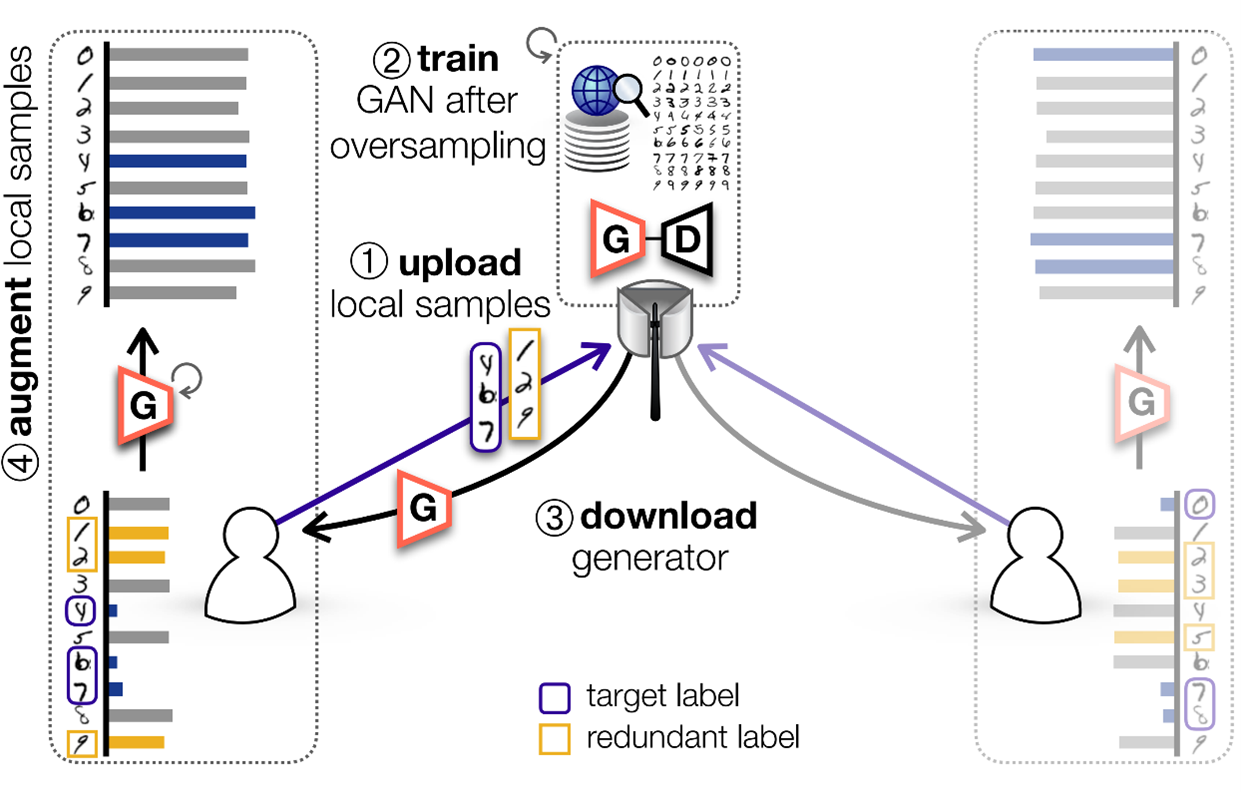
\includegraphics[scale=0.9]{images/chap3/generative_adversarial_network.png}%
	\caption{%
		استفاده از شبکه مولد رقابتی جهت تولید داده
		\cite{jeong2018communication}%
		.
	}
	\label{gan}
	\centering
\end{figure}


\subsection{انتخاب داده}
در هنگام انتخاب کاربران برای فرآیند آموزش، می‌توان از الگوریتم‌هایی که بر پایه کیفیت داده‌ها عمل می‌کنند، استفاده نمود. به عبارت دیگر، می‌توان از الگوریتم حریصانه کوله‌پشتی برای اولویت‌بندی کاربران بهره برد، به نحوی که کاربران با داده‌های غنی و گسترده‌تر، اولویت بالاتری جهت انتخاب داشته باشند. این رویکرد به بهبود کیفیت آموزش کمک می‌کند، زیرا داده‌های با کیفیت بالاتر تاثیر مثبتی بر نتایج نهایی مدل خواهند داشت
\cite{taik2021data}.

علاوه بر این، می‌توان از روش‌های یادگیری عمیق برای تخمین زمان اجرای مدل در سمت کاربران استفاده کرد. این روش‌ها می‌توانند زمان مورد نیاز برای اجرای مدل را پیش‌بینی کنند و بر اساس این پیش‌بینی، از بین ویژگی‌های مختلف جهت آموزش، تنها آن‌هایی را انتخاب نمایند که تاثیر بیشتری بر خروجی خواهند داشت. به این ترتیب، با بهینه‌سازی انتخاب ویژگی‌ها، می‌توان زمان و منابع محاسباتی را به شکل موثرتری مدیریت کرد.

یکی از نکات کلیدی در استفاده از این روش‌های انتخاب داده این است که هیچ کدام از آن‌ها تغییری بر روی داده‌ها و کاربران ایجاد نمی‌کنند. به عبارت دیگر، این روش‌ها به گونه‌ای طراحی شده‌اند که داده‌های موجود و وضعیت کاربران بدون تغییر باقی می‌مانند، اما فرآیند انتخاب و استفاده از داده‌ها بهینه‌تر و کارآمدتر می‌شود. این ویژگی، استفاده از این راه‌حل‌ها را در برنامه‌های مختلف بسیار کاربردی و موثر می‌سازد
\cite{zeng2022local}.

در نتیجه، استفاده از الگوریتم‌های مبتنی بر کیفیت داده‌ها و روش‌های یادگیری عمیق برای تخمین زمان اجرا، می‌تواند به طور قابل توجهی فرآیند آموزش در سیستم‌های یادگیری فدرال را بهبود بخشد. این روش‌ها نه تنها کیفیت داده‌های مورد استفاده را افزایش می‌دهند، بلکه با بهینه‌سازی منابع محاسباتی و زمان اجرا، کارایی سیستم را نیز بهبود می‌بخشند. این ترکیب از بهینه‌سازی داده‌ها و مدیریت منابع، به ویژه در محیط‌های با منابع محدود، اهمیت ویژه‌ای دارد و می‌تواند به نتایج بهتری در آموزش مدل‌ها منجر شود.


\section{نگرش برپایه مدل}
\subsection{
	تجمیع و به‌روزرسانی مدل%
	\protect
	\LTRfootnote{Model Update and Aggregation}
}	
هنگام اجرای الگوریتم در مراحل میانی، می‌توان با استفاده از ساختار شبکه‌های عصبی عمیق موجود، تفاوت گره‌های شبکه بین کاربران مختلف را بررسی نمود. این بررسی به ما امکان می‌دهد تا ساختار مدل اصلی را بر اساس تفاوت‌ها و ویژگی‌های مختلف کاربران، بهبود بخشیم و در نتیجه مدل کارآمدتری ایجاد کنیم. این فرآیند می‌تواند به بهینه‌سازی عملکرد مدل و افزایش دقت آن در مراحل بعدی کمک کند
\cite{sannara2021federated}.

روش دیگری برای بهبود عملکرد یادگیری فدرال این است که هم در سمت سرور و هم در سمت کاربران چندین مدل شبکه عصبی قرار داده شود. این شبکه‌ها به صورت جداگانه آموزش داده شده و به‌روزرسانی می‌شوند. پس از چند مرحله آموزش، می‌توان با استفاده از الگوریتم‌های تطابق بهترین، شبکه‌ها را با یکدیگر ترکیب کرد. این رویکرد به بهبود عملکرد کلی مدل کمک می‌کند و باعث می‌شود تا مدل نهایی از ویژگی‌ها و مزایای چندین شبکه عصبی بهره‌مند شود
\cite{qin2021mlmg}.

همچنین، مکانیزم یادگیری فدرال نیمه-ناهمزمان%
\LTRfootnote{Semi-Asynchronous}
نیز یکی دیگر از روش‌های موثر در این حوزه است. در این روش، مدل‌های کاربران به ترتیبی که به سرور می‌رسند به‌روزرسانی می‌شوند. این رویکرد به خوبی با کاربران کند%
\LTRfootnote{Stragglers}
که ممکن است در گردش‌های مختلف به سرور بپیوندند، سازگار است. با به‌روزرسانی و ترکیب مدل‌ها در مراحل مختلف، این مکانیزم به خوبی می‌تواند توازن را برای داده‌های ناهمگن برقرار کند و عملکرد مدل را بهینه سازد
\cite{ma2021fedsa, ma2022state}.

در نهایت، با استفاده از این رویکردها و الگوریتم‌ها می‌توان به طور موثرتری با چالش‌های موجود در یادگیری فدرال مقابله کرد و مدل‌هایی با دقت و کارایی بالاتر ایجاد نمود. این روش‌ها نه تنها به بهبود ساختار مدل‌ها کمک می‌کنند، بلکه باعث می‌شوند تا فرآیند آموزش بهینه‌تر و سازگارتر با تنوع و ناهمگنی داده‌ها انجام شود.


\subsection{
	بهینه‌سازی تطبیقی%
	\protect
	\LTRfootnote{Adaptive Optimization}
}
الگوریتم پیش‌بینی میزان‌کار به گونه‌ای طراحی شده است که به صورت خودکار اطلاعات جامعی از سابقه آموزش هر کاربر را جمع‌آوری می‌کند. این اطلاعات شامل عملکرد کاربر در مراحل قبلی آموزش است. سپس بر اساس این سوابق، میزان پیچیدگی الگوریتم برای مرحله بعدی آموزش تعیین می‌شود تا برای کاربر مربوطه مناسب باشد . این رویکرد به بهینه‌سازی فرآیند آموزش کمک می‌کند و موجب می‌شود تا الگوریتم‌ها به شکل موثرتری با توانایی‌های هر کاربر هماهنگ شوند
\cite{li2021fedsae}.

یکی از روش‌های اولیه در بهینه‌سازی تطبیقی، استفاده از روش کاهش نرخ یادگیری است. در این روش، نرخ یادگیری برای هر کاربر به طور جداگانه و بر اساس عملکرد گذشته وی تعیین می‌شود. این به معنای آن است که کاربران با عملکرد بهتر ممکن است نرخ یادگیری بالاتری داشته باشند، در حالی که برای کاربرانی که با مشکلاتی مواجه بوده‌اند، این نرخ کاهش می‌یابد تا فرآیند یادگیری بهبود یابد
\cite{reddi2020adaptive}.

در طول سال‌های اخیر، بهینه‌سازی تطبیقی نشان داده است که می‌تواند تاثیر قابل‌توجهی بر بهبود عملکرد الگوریتم‌ها داشته باشد. به همین دلیل، محققان به سمت توسعه روش‌هایی رفته‌اند که امکان تغییر و تطبیق پارامترهای الگوریتم را در طول زمان فراهم کنند. این رویکرد باعث می‌شود تا هر کاربر بتواند در مراحل مختلف آموزش، پارامترهای مربوط به الگوریتم را متناسب با نیازها و شرایط خود تنظیم کند. این انعطاف‌پذیری به الگوریتم‌ها کمک می‌کند تا با گذشت زمان کارایی بیشتری داشته باشند و به طور خاص‌تر با شرایط و نیازهای کاربران سازگار شوند.

به طور کلی، استفاده از الگوریتم‌های پیش‌بینی و بهینه‌سازی تطبیقی می‌تواند به شکل چشم‌گیری کیفیت آموزش و کارایی سیستم‌های یادگیری را بهبود بخشد. این روش‌ها با فراهم کردن امکان تنظیم پارامترهای آموزشی بر اساس سوابق و عملکرد کاربران، موجب می‌شوند تا فرآیند یادگیری به شکل دقیق‌تر و موثرتری انجام شود. در نتیجه، کاربران می‌توانند از تجربیات گذشته خود بهره ببرند و با شرایط بهتر و مناسبتری به یادگیری ادامه دهند.

\subsection{بهینه‌سازی منظم}
از مهم‌ترین و پرکاربردترین روش‌های موجود جهت کنترل داده‌های غیرمستقل و غیریکنواخت، رویکردهای بهینه‌سازی منظم هستند. این رویکردها با هدف بهبود فرآیند یادگیری و کاهش نوسانات ناشی از تفاوت در توزیع داده‌ها به کار گرفته می‌شوند. به عنوان مثال، یکی از روش‌های متداول در این زمینه، در نظر گرفتن نزدیک‌ترین همسایه است که طی آن تابع بهینه‌سازی محلی برای هر کاربر به‌روزرسانی می‌شود تا از نوسانات زیاد جلوگیری کند و هماهنگی بیشتری بین داده‌های مختلف کاربران ایجاد شود
\cite{li2020federatedheteroneneous}.

یکی دیگر از روش‌های معروف در این زمینه، مکانیزم استاد-دانشجو%
\LTRfootnote{Teacher-Student}
است. در این روش، یک مدل به عنوان استاد و مدل‌های دیگر به عنوان دانشجو عمل می‌کنند. گرادیان‌ها برای هر کاربر توسط یک جمله اضافه شده به نام جمله منظم‌سازی%
\LTRfootnote{Regularization Term}
تنظیم می‌شود. این جمله منظم‌سازی به منظور کاهش خطاها و بهبود دقت مدل‌ها افزوده می‌شود و از بیش‌برازش%
\LTRfootnote{Overfitting}
جلوگیری می‌کند
\cite{li2020communication}.

رویکردهای بهینه‌سازی منظم، همان‌طور که در حوزه‌های مختلف یادگیری ماشین و یادگیری عمیق توانسته‌اند کارایی خود را به اثبات برسانند، در یادگیری فدرال نیز عملکرد بسیار خوبی دارند. این رویکردها با تنظیم مدل‌ها به گونه‌ای که نوسانات ناشی از داده‌های مختلف را کاهش دهند، به بهبود عملکرد کلی سیستم کمک می‌کنند. همچنین، با جلوگیری از بیش‌برازش، مدل‌ها را به سمت تعمیم بهتر هدایت می‌کنند، که این امر در محیط‌هایی با داده‌های غیرمستقل و غیریکنواخت بسیار حیاتی است.

در مجموع، استفاده از روش‌های بهینه‌سازی منظم در یادگیری فدرال نه تنها باعث بهبود دقت مدل‌ها می‌شود، بلکه موجب می‌گردد تا فرآیند یادگیری با پایداری و کارایی بیشتری انجام شود. این رویکردها به دلیل توانایی‌شان در کنترل نوسانات و کاهش خطاها، از ابزارهای اساسی در یادگیری فدرال به شمار می‌آیند و به توسعه مدل‌های دقیق و قابل اعتماد کمک می‌کنند.



\section{نگرش برپایه چهارچوب}
\subsection{
	خوشه‌بندی مشابهت%
	\protect
	\LTRfootnote{Similarity Clustering}
}
خوشه‌بندی یکی از روش‌های بسیار پرکاربرد و مهم در حوزه یادگیری ماشین است که ایده‌های آن می‌توانند در یادگیری فدرال نیز مورد استفاده قرار گیرند. در این روش، هنگامی که کاربران مدل‌های خود را آموزش داده و به سرور ارسال می‌کنند، سرور بر اساس مدل‌های دریافتی شباهت‌های آن‌ها را بررسی کرده و کاربرانی که مدل‌های مشابه دارند را در یک خوشه قرار می‌دهد. این فرایند به سرور امکان می‌دهد تا در مراحل بعدی، مدل یکسانی را برای اعضای هر خوشه ارسال کند. این رویکرد باعث می‌شود که مدل‌های آموزش‌دیده شده توسط کاربران با داده‌های مشابه، به طور همزمان و هماهنگ بهبود یابند و از همگرایی بهتری برخوردار شوند
\cite{ghosh2019robust}.

به طور معمول، پس از چندین دوره آموزشی، فرآیند خوشه‌بندی مجدداً تکرار می‌شود تا از به‌روزرسانی‌های جدید و تغییرات احتمالی در داده‌ها و مدل‌ها بهره‌برداری شود. در شکل
\ref{similarity_clustering}%
، حالت کلی خوشه‌بندی شباهت در سیستم‌های فدرال به تصویر کشیده شده است.

با وجود تمام مزایایی که روش خوشه‌بندی مشابهت به همراه دارد، یکی از مهم‌ترین مشکلات آن هزینه بالای ارتباطات است. در این روش، نیاز است که ساختار خوشه‌بندی در مراحل مختلف ارسال و دریافت شود، که این فرایند می‌تواند هزینه زیادی را بر شبکه اعمال کند. به خصوص در محیط‌هایی با تعداد زیاد کاربران و داده‌های بزرگ، این هزینه‌ها به طور قابل توجهی افزایش می‌یابد و می‌تواند عملکرد کلی سیستم را تحت تأثیر قرار دهد.

بنابراین، در حالی که خوشه‌بندی شباهت می‌تواند کارایی و دقت یادگیری فدرال را بهبود بخشد، باید به دقت هزینه‌های ارتباطی آن نیز مورد ارزیابی قرار گیرد و در صورت امکان، بهینه‌سازی‌های لازم انجام شود تا این هزینه‌ها کاهش یابند. به کارگیری روش‌های بهینه‌سازی ارتباطات و فشرده‌سازی داده‌ها می‌تواند در این زمینه مفید باشد و به حفظ تعادل بین کارایی و هزینه‌ها کمک کند.

\begin{figure}[t]
	\centering
	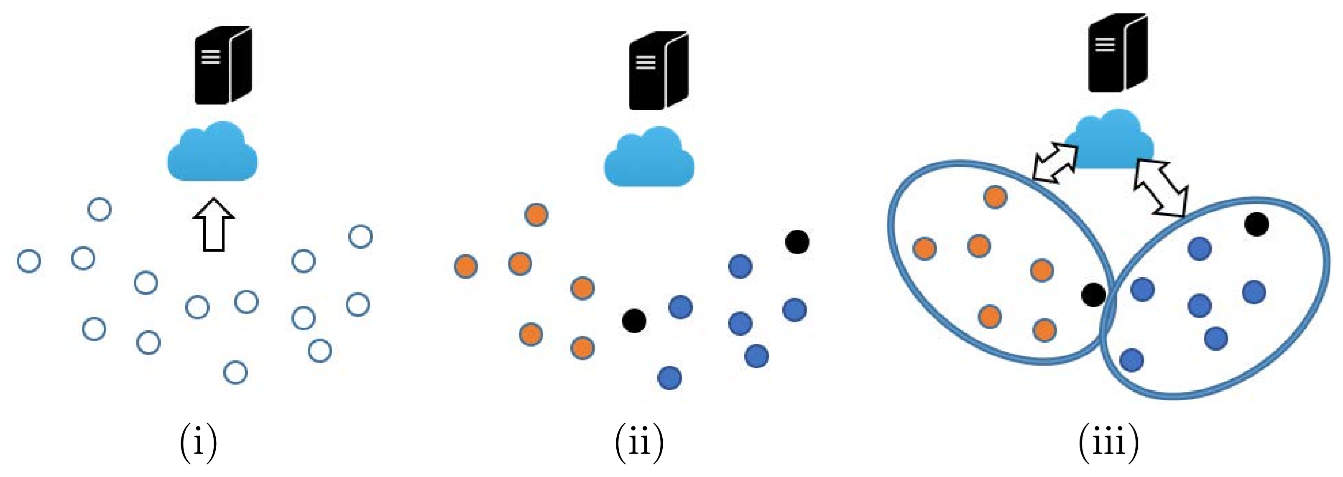
\includegraphics[scale=0.9]{images/chap3/similarity_clustering.png}%
	\caption{%
		روش خوشه‌بندی مشابهت 
		\cite{ghosh2019robust}%
		.
	}
	\label{similarity_clustering}
	\centering
\end{figure}

\subsection{
	دانش تقطیر%
	\protect
	\LTRfootnote{Knowledge Distillation}
}
به‌طور کلی، در روش‌های دانش تقطیر، هدف اصلی ساده‌سازی مدل‌های پیچیده و ارائه مدل‌هایی ساده اما کارآمد است. یکی از الگوریتم‌های مهم در این زمینه
\lr{DS-FL}%
\LTRfootnote{Distillation-base Semi-supervised Federated Learning}
است. این الگوریتم با استفاده از مجموعه داده‌های بدون برچسب، به جای ارسال پارامترهای مدل، تنها خروجی مدل محلی را به اشتراک می‌گذارد. این روش به‌خصوص برای داده‌های غیرمستقل و غیریکنواخت بسیار مؤثر عمل می‌کند و نتایج مطلوبی به همراه دارد.

یکی از مهم‌ترین مزایای استفاده از دانش تقطیر، کاهش چشمگیر سربار شبکه است. به دلیل اینکه در این روش به جای ارسال پارامترهای مدل‌های محلی، فقط خروجی نهایی مدل‌ها ارسال می‌شود، حجم داده‌های ارسالی به طور قابل توجهی کاهش می‌یابد. این کاهش حجم داده‌ها نه تنها هزینه‌های ارتباطی را پایین می‌آورد بلکه سرعت پردازش و به‌روزرسانی مدل‌ها را نیز افزایش می‌دهد. به این ترتیب، بهره‌وری سیستم بهبود یافته و توان محاسباتی به نحو بهتری مدیریت می‌شود.

در روش
\lr{DS-FL}%
، ابتدا هر کاربر محلی با استفاده از داده‌های خود، مدلی را آموزش می‌دهد. سپس به جای ارسال پارامترهای مدل به سرور مرکزی، تنها خروجی مدل روی داده‌های بدون برچسب به اشتراک گذاشته می‌شود. سرور مرکزی با تجمیع این خروجی‌ها، یک مدل جهانی به‌روز شده را ایجاد می‌کند و آن را برای کاربران ارسال می‌کند. این فرایند تکرار می‌شود تا مدل جهانی به بهینه‌ترین حالت ممکن برسد
\cite{itahara2021distillation}.

به کارگیری دانش تقطیر در یادگیری فدرال نه تنها به بهبود کارایی شبکه کمک می‌کند، بلکه امنیت و حریم خصوصی داده‌ها را نیز افزایش می‌دهد. چون خروجی مدل‌ها اغلب اطلاعات حساس کمتری نسبت به پارامترهای مدل در خود دارند، احتمال افشای اطلاعات شخصی کاربران کاهش می‌یابد. این ویژگی به‌خصوص در محیط‌هایی که حفظ حریم خصوصی کاربران اولویت بالایی دارد، از اهمیت ویژه‌ای برخوردار است.

به‌طور خلاصه، روش‌های دانش تقطیر مانند
\lr{DS-FL}
با هدف ساده‌سازی مدل‌های پیچیده و کاهش هزینه‌های ارتباطی، به بهبود کارایی و امنیت در سیستم‌های یادگیری فدرال کمک می‌کنند. این روش‌ها با ارسال خروجی‌های مدل به جای پارامترها، سربار شبکه را کاهش داده و به تطبیق بهتر مدل‌ها با داده‌های غیرمستقل و غیریکنواخت کمک می‌کنند.


\subsection{
	لایه‌های شخصی‌سازی%
	\protect
	\LTRfootnote{Personalization Layers}
}
روش لایه‌های شخصی‌سازی شده به این شکل عمل می‌کنند که در ابتدا کاربران بر اساس معیارهایی مانند کارایی آموزش و سرعت اجرا به گروه‌های مختلفی تقسیم می‌شوند. سپس، این کاربران بر اساس معیارهای تعیین شده به صورت لایه‌ای مرتب می‌شوند. به این ترتیب، سرور هنگامی که مدل را به‌روزرسانی می‌کند و قصد دارد آن را در مرحله بعد به سمت کاربران ارسال نماید، سعی می‌کند کاربرانی را که در یک لایه مشترک حضور دارند انتخاب کند. این انتخاب به سرور امکان می‌دهد تا گردش به‌روزرسانی‌ها را با سرعت و کارایی هماهنگ‌تری به پایان برساند و عملکرد بهتری از سیستم بگیرد
\cite{chai2020tifl}.

یکی از نکات کلیدی در اجرای این روش، تعیین میزان حد و آستانه‌ای است که بر اساس آن، کاربران به لایه‌های مختلف تقسیم می‌شوند. این تقسیم‌بندی باید به گونه‌ای باشد که خروجی مدل بهینه باشد و کارایی سیستم حفظ شود. تعیین این حد و آستانه‌ها می‌تواند چالش‌برانگیز باشد و نیاز به سعی و خطا دارد تا بهترین ترکیب ممکن به دست آید.

به‌طور کلی، روش لایه‌های شخصی‌سازی شده با تقسیم‌بندی کاربران و مرتب‌سازی آن‌ها در لایه‌های مختلف، امکان بهبود هماهنگی و کارایی در گردش به‌روزرسانی‌ها را فراهم می‌کند. این رویکرد نه تنها باعث می‌شود که کاربران با سرعت مشابه در یک لایه قرار گیرند، بلکه به سرور کمک می‌کند تا با کاهش ناهماهنگی‌ها، به‌روزرسانی مدل‌ها را با کارایی بیشتری انجام دهد. انتخاب صحیح معیارهای تقسیم‌بندی و آستانه‌ها در این روش، از اهمیت بالایی برخوردار است و نیازمند تحلیل و ارزیابی دقیق است تا بهترین نتایج ممکن به دست آید.




\section{نگرش برپایه الگوریتم}
\subsection{فرایادگیری}
مدل ابتدایی فرایادگیری پیاده‌شده بر بستر یادگیری فدرال، در واقع از همان الگوریتم
\lr{FedAvg}
بهره می‌برد و با ترکیب آن با روش فرایادگیری، تلاش دارد تا فرایند آموزش را بهینه‌سازی کرده و پارامترهای مناسب‌تری را به دست آورد
\cite{jiang2019improving}.
الگوریتم اولیه-دوگانه%
\LTRfootnote{Primal-Dual}
\lr{(FedPD)}%
، یکی از الگوریتم‌های کارا با استفاده از فرایادگیری است که حتی برای توابع نامحدب%
\LTRfootnote{Nonconvex}
نیز مقاوم بوده و علاوه بر دستیابی به همگرایی مناسب، از نظر کاهش ارتباطات نیز بسیار کارآمد عمل می‌کند
\cite{zhang2021fedpd}.

روش‌های فرایادگیری به دلیل توانایی‌شان در هماهنگی سریع با داده‌های جدید و تغییر پارامترهای مربوطه، مورد توجه قرار گرفته‌اند. این روش‌ها می‌توانند به سرعت با شرایط جدید سازگار شوند و پارامترهای مدل را بهبود بخشند. با این حال، یکی از چالش‌های اصلی این روش‌ها مربوط به کاربران کند است. این کاربران ممکن است به دلیل محدودیت‌های سخت‌افزاری یا مشکلات ارتباطی، نتوانند به‌روزرسانی‌های سریع و هماهنگ را انجام دهند و این موضوع می‌تواند باعث اختلال در عملکرد مدل شود.

به طور کلی، مدل‌های فرایادگیری در بستر یادگیری فدرال با ترکیب روش‌های مختلف و بهره‌گیری از الگوریتم‌های بهینه‌سازی مانند
\lr{FedAvg}
و
\lr{FedPD}%
، سعی دارند تا با بهبود فرآیندهای آموزش و کاهش هزینه‌های ارتباطی، به نتایج بهتری دست یابند. این روش‌ها با وجود چالش‌هایی که ممکن است در پیاده‌سازی و هماهنگی با کاربران کند داشته باشند، به دلیل قابلیت‌هایشان در بهینه‌سازی و هماهنگی سریع با داده‌های جدید، پتانسیل بالایی برای بهبود عملکرد سیستم‌های یادگیری فدرال دارند.

\subsection{یادگیری چندوظیفه‌ای}
یادگیری چندوظیفه‌ای به این معناست که هر یک از کاربران شرکت‌کننده در فرآیند یادگیری فدرال، به دنبال یادگیری وظایف مختلفی هستند و تلاش می‌شود که در این مسیر، حریم شخصی کاربران به طور قابل‌توجهی حفظ شود. در یادگیری فدرال چندوظیفه‌ای، کاربران بر اساس داده‌های محلی خود، مدل را آموزش می‌دهند و نتایج آن را به سمت سرور مرکزی ارسال می‌کنند. سپس سرور، با تحلیل پارامترهای ارسال شده، روابط معناداری میان این مدل‌ها پیدا کرده و مدل به‌روز شده را دوباره به سمت کاربران بازمی‌گرداند
\cite{corinzia2019variational}.

به عبارت دیگر، در این روش، هر کاربر ابتدا مدل را با استفاده از داده‌های محلی خود آموزش می‌دهد. این فرآیند موجب می‌شود که داده‌های شخصی کاربران از دستگاه‌های آنان خارج نشود و فقط نتایج به دست آمده از مدل‌های محلی به سرور ارسال شود. سرور مرکزی با جمع‌آوری این نتایج، به دنبال یافتن الگوها و روابطی است که بتواند مدل کلی را بهبود بخشد. این مدل بهبود یافته سپس به کاربران ارسال می‌شود تا مجدداً با داده‌های محلی آنان آموزش داده شود.

در شکل
\ref{multi_tasking}%
، نمای کلی از نحوه عملکرد یادگیری چندوظیفه‌ای در سیستم‌های فدرال به نمایش گذاشته شده است. این شکل به خوبی نشان می‌دهد که چگونه هر کاربر با استفاده از داده‌های محلی خود مدل را آموزش داده و نتایج را به سرور ارسال می‌کند و سرور با تحلیل این نتایج، مدل بهبود یافته را به کاربران بازمی‌گرداند.

به طور کلی، یادگیری چندوظیفه‌ای فدرال، به دلیل توانایی‌اش در تطبیق با داده‌های متنوع و محافظت از حریم خصوصی کاربران، یک رویکرد بسیار مؤثر و کارآمد در زمینه یادگیری فدرال محسوب می‌شود.

\begin{figure}[t]
	\centering
	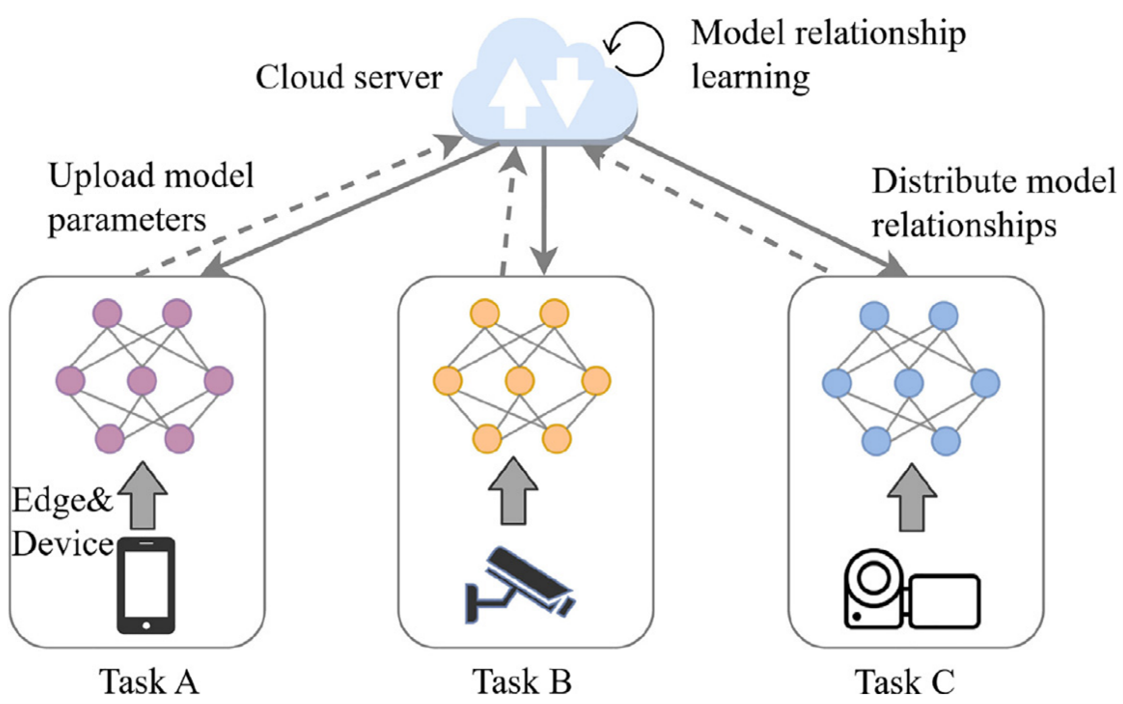
\includegraphics[scale=0.9]{images/chap3/multi_tasking.png}%
	\caption{%
		یادگیری فدرال چندوظیفه‌ای
		\cite{ma2022state}%
		.
	}
	\label{multi_tasking}
	\centering
\end{figure}


\subsection{
	یادگیری مادام‌العمر%
	\protect
	\LTRfootnote{Life-Long Learning}
}
رویکرد اصلی یادگیری مادام‌العمر به این صورت است که تلاش می‌کند در هر مرحله از الگوریتم، کاربرانی که برای اجرا انتخاب می‌شوند را به خاطر بسپارد. همان‌طور که پیش‌تر مطرح شد، در یادگیری فدرال ممکن است در هر مرحله تعداد کمی از کاربران انتخاب شوند. این مسئله باعث می‌شود که وزن‌ها و مدل‌هایی که برای کاربران جدید ارسال می‌شوند، لزوماً کارایی لازم را نداشته باشند. الگوریتم یادگیری مادام‌العمر تلاش دارد تا کاربران را به‌خاطر بسپارد و مدل‌های متناسب با هر کدام را ایجاد و به سمت آن‌ها ارسال کند
\cite{shoham2019overcoming}.

این رویکرد به این صورت عمل می‌کند که در هر مرحله از یادگیری، سوابق کاربران انتخاب شده را ذخیره می‌کند و از این سوابق برای بهبود و تطبیق مدل‌های آینده استفاده می‌کند. به این ترتیب، زمانی که کاربر جدیدی وارد فرآیند یادگیری می‌شود، الگوریتم می‌تواند از اطلاعات ذخیره شده قبلی استفاده کند و مدل بهتری را برای او ارسال کند. این روش باعث می‌شود که مدل‌ها به مرور زمان بهینه‌تر شده و عملکرد بهتری داشته باشند.

یکی از نکات مهم در یادگیری مادام‌العمر، حفظ و به‌خاطر سپاری کاربران است. در زمینه یادگیری فدرال، این کار به دلیل تعداد بسیار زیاد کاربران ممکن است چالش‌برانگیز باشد. یادگیری فدرال به‌طور معمول با تعداد زیادی از کاربران سروکار دارد و حفظ سوابق همه این کاربران به‌طور همزمان می‌تواند منابع زیادی را مصرف کند و پیچیدگی‌های فنی زیادی را به همراه داشته باشد.

در نتیجه، یادگیری مادام‌العمر با ذخیره و استفاده از اطلاعات کاربران در طول زمان، می‌تواند به طور مؤثری به مدیریت چالش‌های مربوط به داده‌های غیرمستقل و غیریکنواخت در یادگیری فدرال کمک کند و همچنین به حفظ و بهبود کارایی مدل‌های یادگیری فدرال کمک نماید.




% Chapter 4
\chapter{روش پیشنهادی برای جابه‌جایی مدل‌های شبکه عصبی بین کاربران}

\section{مقدمه}
در فصل گذشته، به بررسی روش‌های گوناگون برای مقابله با مشکل داده‌های 
\lr{non-IID}
در یادگیری فدرال پرداخته شد. در این فصل، تلاش خواهد شد با استفاده از جابه‌جایی مدل‌های شبکه عصبی بین کاربران نهایی، راهکاری برای پیاده‌سازی یادگیری فدرال بر روی داده‌های 
\lr{non-IID}
ارائه شود. شکل 
\ref{iid_vs_noniid}
به‌خوبی مفهوم داده‌های 
\lr{non-IID}
را توضیح می‌دهد، اما برای این که روشن شود چگونه جابه‌جایی مدل‌ها می‌توانند در این زمینه مؤثر باشند، در این بخش یک مثال مناسب ارائه می‌شود.

فرض کنید که هدف، آموزش مدلی برای شناسایی اشیائی مانند علائم ترافیکی و تابلوهای فروشگاهی است. اگر وسایل نقلیه، یکی در بزرگراه و دیگری در مرکز شهر حرکت کنند، داده‌های ویدیویی آن‌ها توزیع‌های متفاوتی از این علائم و تابلوها را ثبت خواهند کرد. به این صورت که داده‌های جمع‌آوری شده از بزرگراه، احتمالاً تابلوهای فروشگاهی کمتری را شامل می‌شود، در حالی که داده‌های ثبت شده در مرکز شهر حاوی تعداد بیشتری از هر دو نوع علائم و تابلوها هستند. این اختلاف توزیع داده‌ها در دستگاه‌های مختلف، می‌تواند منجر به مشکل انحراف در وزن‌دهی مدل شود.

برای حل این مسئله در پژوهش‌های پیشین، عملیات جابه‌جایی مدل‌های شبکه عصبی بین کاربران پیشنهاد شده است. این رویکرد، مدل‌ها را بین دستگاه‌های نهایی جابه‌جا می‌کند تا تنوع داده‌ها در دستگاه‌های مختلف کاهش یابد. این فرایند با تحمیل هزینه اندک به منابع محاسباتی و ارتباطی، باعث بهبود مدل در برخورد با داده‌های  
\lr{non-IID}  
می‌شود.

در این فصل، ابتدا به معرفی روش جابه‌جایی مدل‌ها پرداخته می‌شود که شامل دو نوع جابه‌جایی تصادفی و بر پایه شباهت است. روش جابه‌جایی بر ‎پایه شباهت، در واقع همان رویکرد پیشنهادی این پژوهش محسوب می‌شود.
سپس، تاثیرات این جابه‌جایی‌ها بر ترافیک شبکه و حفظ حریم شخصی، مورد بررسی قرار می‌گیرد. در ادامه، معیارهای مشابهت و پایداری آن‌ها تعریف و ارزیابی می‌شوند. در پایان، شاخص‌های مشابهت بین شبکه‌های عصبی مشخص شده و دو روش اصلی برای انتخاب کاربران جهت جابه‌جایی مدل‌ها تحلیل می‌شوند.

%در این فصل، ابتدا به مرور روش پیشین جابه‌جایی مدل‌ها پرداخته می‌شود که این روش با عنوان روش جابه‌جایی تصادفی شناخته می‌شود. پس از آن روش پیشنهادی در این پژوهش با عنوان جابه‌جایی بر پایه شباهت معرفی می‌شود. در ادامه، تاثیرات هر یک از این روش‌ها بر ترافیک شبکه و حفظ حریم شخصی، مورد بررسی قرار می‌گیرد. علاوه بر این، معیارهای مشابهت و پایداری آن‌ها تعریف و ارزیابی می‌شوند. در پایان، شاخص‌های مشابهت بین شبکه‌های عصبی مشخص شده و دو روش اصلی برای انتخاب کاربران جهت جابه‌جایی مدل‌ها تحلیل می‌شوند.

\section{
	روش جابه‌جایی فدرال%
	\LTRfootnote{Federated Swapping}
	\lr{\texttt{\fontspec{Times New Roman} (FedSwap)}}
}
در این روش، یک عملیات جدید به نام جابه‌جایی فدرال یا
\lr{FedSwap}
پیشنهاد شده است که به عنوان جایگزینی برای برخی از دوره‌های
\lr{FedAvg}
در یادگیری فدرال به کار می‌رود.
این عملیات با هدف بهبود فرآیند یادگیری فدرال و کاهش تاثیرات منفی داده‌های
\lr{non-IID}
طراحی شده است
\cite{chiu2020semisupervised}.


در روش‌ یادگیری فدرال، پس از هر تکرار، مدل‌های محلی از دستگاه‌های نهایی جمع‌آوری شده و یک مدل جامع از ترکیب آن‌ها ساخته می‌شود. اما در روش
\lr{FedSwap}%
، به‌جای این که این ادغام در هر تکرار انجام شود، سرور مدل‌های محلی را در گام‌های مشخصی بین دستگاه‌ها جابه‌جا می‌کند. در واقع، در انتهای برخی مراحل، عملیات جابه‌جایی و در انتهای برخی دیگر، ادغام مدل‌ها صورت می‌گیرد. این مراحل بر اساس پارامترهایی که به عنوان ورودی تعریف می‌شوند، تعیین می‌گردند.
جهت درک بهتر این ساختار به شکل
\ref{federated_swapping}
توجه نمایید.


\begin{figure}[b!]
	\centering
	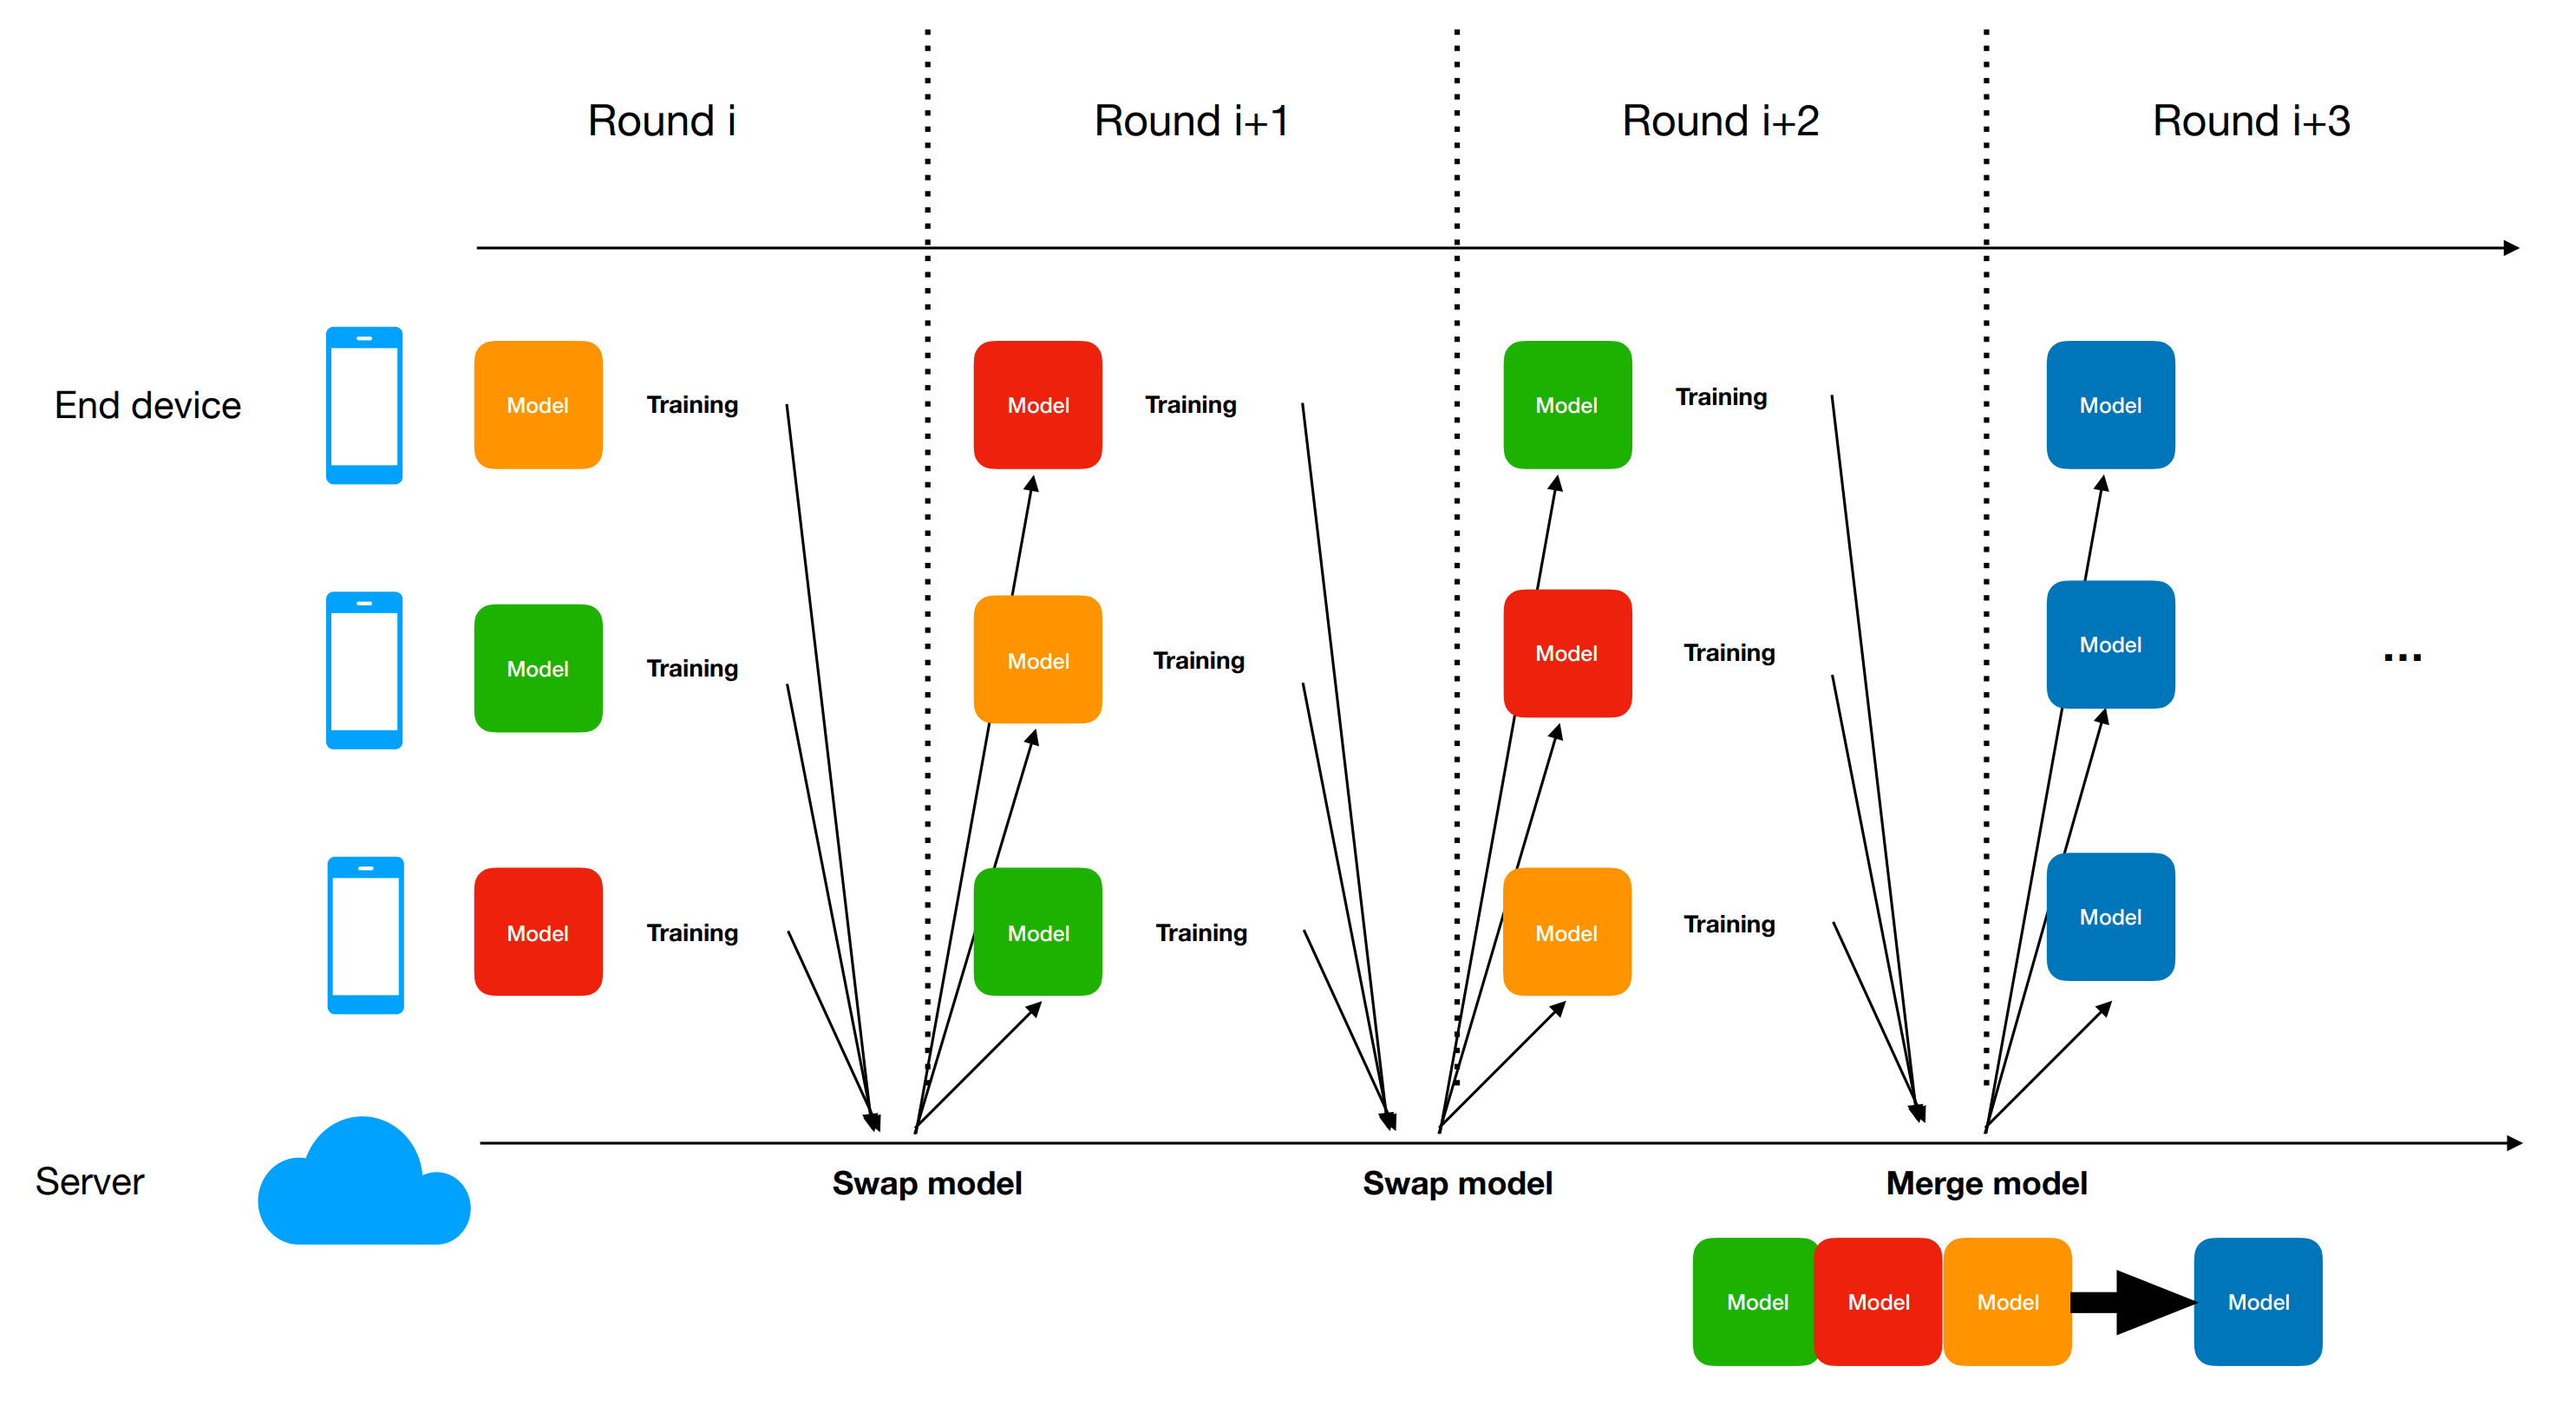
\includegraphics[scale=0.179]{images/chap4/federated_swapping.png}%
	\caption{%
		روش جابه‌جایی فدرال
		\cite{chiu2020semisupervised}%
		.
	}
	\label{federated_swapping}
	\centering
\end{figure}


برای حفظ توازن در این فرآیند، از یک استراتژی چرخشی%
\LTRfootnote{Cyclic}
استفاده می‌شود. در این استراتژی، به‌طور منظم، دو دستگاه نهایی به یکدیگر اجازه می‌دهند که مدل‌های خود را تبادل کنند. این کار باعث می‌شود که همه دستگاه‌های نهایی به‌طور مساوی در فرآیند تبادل مدل‌ها شرکت کنند و هیچ دستگاهی از مزایای این تبادل محروم نماند.

علاوه بر این، انتظار می‌رود که این عملیات جابه‌جایی مدل بین دستگاه‌های نهایی، به هر مدل دید گسترده‌تری از کل مجموعه داده‌ها بدهد. به عبارت دیگر، هر مدل محلی با تبادل مدل با دیگر دستگاه‌ها، می‌تواند اطلاعات بیشتری از داده‌های مختلف دریافت کند. این امر به کاهش انحراف وزن‌ها کمک می‌کند، زیرا مدل‌ها با داده‌های متنوع‌تری آموزش می‌بینند و به تدریج به یک مدل جامع‌تر و دقیق‌تر نزدیک می‌شوند.

به‌طور خلاصه، روش
\lr{FedSwap}
با تبادل مدل‌های محلی بین دستگاه‌های نهایی، نه تنها به بهبود دقت و عملکرد مدل‌ها کمک می‌کند، بلکه مشکلات ناشی از داده‌های
\lr{non-IID}
را نیز کاهش می‌دهد. این روش به عنوان یک رویکرد موثر در یادگیری فدرال می‌تواند باعث بهبود قابل توجهی در نتایج نهایی شود
\cite{chiu2020semisupervised}.


جزئیات عملیات
\lr{FedSwap}
در الگوریتم
\ref{algo_FedSwap}
ارائه شده است.
همچنین در جدول
\ref{tabel_FedSwapNotations}
نمادهای مختص این الگوریتم به نمایش در آمده است.
در این الگوریتم،
$w^k_t$
به عنوان وزن مدل در دستگاه نهایی
$k$
پس از گام
$t$
تنظیم می‌شود. در ابتدا، دستگاه‌های نهایی چندین به‌روزرسانی محلی انجام می‌دهند تا مدل‌های خود را بهبود بخشند. پس از هر
$h_1$
مرحله، سرور وارد عمل شده و عملیات جابه‌جایی را اجرا می‌کند. در این مرحله، مدل‌های محلی بین دستگاه‌های نهایی تبادل می‌شوند تا هر دستگاه بتواند از مدل‌های متنوع‌تری برای آموزش استفاده کند.

این تبادل مدل‌ها به کاهش تنوع داده‌ها بین دستگاه‌های مختلف کمک می‌کند و باعث می‌شود که مدل‌ها با داده‌های مختلفی آموزش ببینند. پس از انجام
$h_2$
عملیات جابه‌جایی، سرور وارد عمل شده و عملیات میانگین‌گیری را اجرا می‌کند. در این مرحله، سرور مدل‌های محلی را تجمیع می‌کند تا یک مدل مشترک ایجاد شود که از داده‌های تمام دستگاه‌ها بهره‌ می‌برد.


\begin{LTR}
	\SetAlgoNlRelativeSize{-1}
	\begin{algorithm}[t]
		\begin{RTL}
			\caption{%
				جابه‌جایی فدرال
				\lr{(FedSwap)}
				\cite{chiu2020semisupervised}
			}
			\label{algo_FedSwap}
		\end{RTL}
		
		\begin{latin}
			Initialize all clients model with weight $w_0$\;
			\For{$t = 1, 2, \ldots, T$}{
				\For{each client $k = 1, 2, \ldots, K$
					\textbf{in parallel}}{
					$w_t^k = w_{t-1}^k - \eta \nabla F(w_{t-1}^k)$\;
				}
				\If{$t|h_1 = 0$ \quad and \quad $t|h_1h_2 \neq 0$}{
					\For{each client $k = 1, 2, \ldots, K$}{
						$w_t^k \gets \texttt{Swapping}(k, \{w_t^k\}_{k \in K})$\;
					}
				}
				\If{$t|h_1h_2 = 0$}{
					$w_t \gets \texttt{WeightedAvg}(\{w_t^k\}_{k \in K})$\;
					\For{each client $k = 1, 2, \ldots, K$
						\textbf{in parallel}}{
						$w_t^k \gets w_t$\;
					}
				}
			}
			\SetKwFunction{Swapping}{Swapping}
			\SetKwFunction{WeightedAvg}{WeightedAvg}
			\SetKwProg{Fn}{Function}{:}{end}
			\Fn{\Swapping{$k, \{w_t^k\}_{k \in K}$}}{
				$r$ \space represent a random client in \space $K$\;
				$w_t \gets w_t^r$\;
				$w_t^r \gets w_t^k$\;
				\KwRet $w_t$\;
			}
			\Fn{\WeightedAvg{$\{w_t^k\}_{k \in K}$}}{
				$w_t \gets \sum_{k=1}^K \frac{n_k}{n} w_t^k$\;
				\KwRet $w_t$\;
			}
		\end{latin}
	\end{algorithm}
\end{LTR}


\begin{table}[h]
	\centering
	\caption{نمادهای مختص الگوریتم
		\lr{FedSwap}
	}
	\label{tabel_FedSwapNotations}
	\begin{tabular}{cr}
		\hline
		متغیر & توضیحات \\
		\hline
		$h_1$ & تعداد گام‌ها بین هر جابه‌جایی \\
		$h_2$ & تعداد جابه‌جایی‌ها بین هر میانگین‌گیری
	\end{tabular}
\end{table}


برای تعیین مقادیر
$h_1$
و
$h_2$%
، ابتدا آزمایش‌های مختلفی انجام شده و بر اساس نتایج به دست آمده به‌صورت تجربی، مقادیر نهایی انتخاب شده‌اند. در این آزمایش‌ها، چند نکته مهم مشاهده شده است. ابتدا، مقدار
$h_1$
به عملکرد به‌روزرسانی مدل محلی در دستگاه‌های نهایی وابسته است. از آن‌ جایی که وظیفه یادگیری معمولاً یک وظیفه عمومی مثل طبقه‌بندی است، مقدار
$h_1$
بر اساس مقدار گام تعریف‌شده در روش میانگین‌گیری فدرال سنتی تنظیم می‌شود
\cite{chiu2020semisupervised}.

علاوه بر این، مقدار
$h_2$
نقش مهمی در توازن بین سربار ارتباطی و همگرایی مدل ایفا می‌کند. با افزایش مقدار
$h_2$%
، تعداد دفعات جابه‌جایی فدرال بین دستگاه‌های نهایی بیشتر خواهد شد. این امر می‌تواند با کاهش تعداد دفعات ادغام فدرال، صرفه‌جویی بیشتری در پهنای باند ارتباطی ایجاد کند. با این حال، این امر ممکن است باعث افزایش احتمال انحراف وزن‌ها و کاهش دقت همگرایی مدل سراسری شود. به عبارت دیگر، هرچه مقدار
$h_2$
بزرگتر باشد، تعداد دفعاتی که مدل‌ها بین دستگاه‌های نهایی جابه‌جا می‌شوند بیشتر است و این ممکن است به بهبود عملکرد مدل‌ها در مواجهه با داده‌های
\lr{non-IID}
کمک کند، اما ریسک انحراف وزن‌ها نیز بیشتر خواهد شد، زیرا مرحله ادغام مدل‌ها به تاخیر خواهد افتاد.

از سوی دیگر، اگر مقدار
$h_2$
کوچکتر باشد، فراوانی جابه‌جایی فدرال بین دستگاه‌های نهایی کاهش می‌یابد. این امر منجر به افزایش سربارهای ارتباطی می‌شود، زیرا نیاز به ادغام مکرر مدل سراسری خواهد بود. بنابراین، مقدار
$h_2$
باید به گونه‌ای تنظیم شود که توازن مناسبی بین کاهش سربار ارتباطی و حفظ دقت مدل ایجاد کند.

در مجموع، روش
\lr{FedSwap}
با جابه‌جایی مدل‌های محلی بین دستگاه‌های نهایی بدون نیاز به هزینه‌های محاسباتی و ارتباطی اضافی، می‌تواند به بهبود عملکرد مدل‌ها در مواجهه با داده‌های
\lr{non-IID}
کمک کند
\cite{chiu2020semisupervised}.



\section{نحوه جابه‌جایی مدل‌ها در یادگیری فدرال}
در این بخش، دو روش متفاوت برای جابه‌جایی مدل‌ها در یادگیری فدرال مورد بررسی قرار می‌گیرد. روش جابه‌جایی تصادفی که مدل‌ها را بر حسب تصادف بین دستگاه‌ها جابه‌جا می‌کند و روش مبتنی بر شباهت که با مقایسه مدل‌ها بر اساس شباهت‌ها و تفاوت‌ شبکه‌های عصبی، تصمیم به مبادله می‌گیرد. هر دو روش به منظور ارتقای عملکرد مدل‌ها در شرایطی که داده‌ها
\lr{non-IID}
هستند، طراحی شده‌اند.

\subsection{
روش جابه‌جایی فدرال به‌صورت تصادفی
}

در الگوریتم
\lr{FedSwap}%
، مدل‌های محلی به‌طور کاملاً تصادفی بین دستگاه‌های نهایی مبادله می‌شوند. به بیان دیگر، هر بار که قرار است دو دستگاه مدل‌های خود را با یکدیگر مبادله کنند، انتخاب این دستگاه‌ها به‌صورت تصادفی صورت می‌گیرد. این باعث می‌شود که هیچ الگوی ثابتی در جابه‌جایی مدل‌ها وجود نداشته باشد و در هر مرتبه، ترکیب جدیدی از دستگاه‌ها در فرآیند تبادل مدل‌ها شرکت کنند.


یکی از ویژگی‌های مهم الگوریتم
\lr{FedSwap}%
، این است که تمام دستگاه‌های نهایی به‌صورت مساوی در فرآیند جابه‌جایی شرکت می‌کنند. به عبارت دیگر، همه دستگاه‌های شرکت کننده در این مرحله از اجرا، در فرآیند جابه‌جایی قرار می‌گیرند، اما انتخاب دستگاه‌ها برای جابه‌جایی به‌صورت تصادفی صورت می‌پذیرد. این باعث می‌شود که تمامی دستگاه‌ها فرصت مساوی برای تبادل مدل‌ها و بهبود دقت و عملکرد خود داشته باشند.

با استفاده از این رویکرد، الگوریتم
\lr{FedSwap}
قادر است به بهبود عملکرد مدل‌های محلی کمک کند، زیرا تبادل تصادفی مدل‌ها بین دستگاه‌ها باعث می‌شود که هر دستگاه به داده‌ها و اطلاعات بیشتری دسترسی پیدا کند. این امر به کاهش انحراف وزن‌ها و بهبود همگرایی مدل سراسری کمک می‌کند.


\subsection{
روش پیشنهادی جابه‌جایی فدرال بر پایه شباهت%
	\LTRfootnote{Similarity-based Federated Swapping}
	\lr{\texttt{\fontspec{Times New Roman} (SimFedSwap)}}%
}
همان‌گونه که پیش‌تر بیان شد، هدف اصلی این پژوهش، انتخاب دستگاه‌های نهایی بر اساس میزان شباهت مدل‌های شبکه عصبی و جابه‌جایی آن‌ها با یکدیگر است. برای این منظور، باید به‌طور کامل با ساختار شبکه عصبی آشنا بوده و مدل‌های مختلف را با یکدیگر مقایسه کرد. این مقایسه امکان ارزیابی میزان شباهت و تفاوت بین مدل‌های شبکه عصبی را فراهم می‌کند.

بعد از بررسی و تعیین میزان شباهت مدل‌ها، باید تصمیم گرفت که کدام یک از آن‌ها را با یکدیگر جابه‌جا نمود. در روش پیشنهادی
\lr{SimFedSwap}
بهترین انتخاب برای جابه‌جایی، مدلی است که کمترین شباهت را با مدل شبکه عصبی دستگاه فعلی دارد. دلیل این انتخاب این است که اگر مدل دستگاه فعلی با مدل دستگاه مقصد شباهت زیادی داشته باشد، جابه‌جایی آن‌ها مؤثر نخواهد بود. این شباهت بالا به این معناست که این دو دستگاه نهایی داده‌های مشابهی داشته و در طول زمان آموزش‌های مشابهی دیده‌اند، در نتیجه جابه‌جایی مدل‌ها تأثیر قابل‌توجهی بر بهبود یادگیری نخواهد داشت.

بنابراین، برای توضیح دلیل ارائه این روش، می‌توان به این نکته اشاره کرد که جابه‌جایی مدل‌هایی که کمترین شباهت را بین دستگاه‌های مختلف دارند، به بهبود فرآیند یادگیری کمک خواهند کرد. این فرض بر این اساس است که دستگاه‌هایی با مدل‌های متفاوت، احتمالاً داده‌هایی با ساختارهای متفاوت دارند. پس جابه‌جایی مدل‌ها بین این دستگاه‌ها، مدل‌ها را با داده‌های جدیدی روبه‌رو می‌کند که می‌تواند به یادگیری بهتر و متنوع‌تر کمک کند. در نتیجه، مدل سراسری سریع‌تر به سمت مسیر بهینه همگرا می‌شود و دقت و کارایی آن افزایش می‌یابد.

این روش نه تنها تنوع داده‌ها را در فرآیند یادگیری افزایش می‌دهد، بلکه به کاهش انحراف وزن‌ها نیز کمک می‌کند. با داشتن دید گسترده‌تری از داده‌ها و تجربیات مختلف، مدل‌ها می‌توانند بهتر و جامع‌تر آموزش ببینند. این امر در نهایت منجر به بهبود عملکرد کلی مدل در شرایط واقعی می‌شود و کمک می‌کند که مدل‌های یادگیری فدرال بتوانند با چالش‌های داده‌های
\lr{non-IID}
به نحو بهتری مقابله کنند.


نحوه مدیریت بار محاسباتی در روش
\lr{SimFedSwap}
به این صورت است که ابتدا تمام مدل‌های شبکه عصبی از دستگاه‌های نهایی به سمت سرور ارسال می‌شوند. سپس سرور بر اساس معیارهای مشخصی، شباهت بین این مدل‌ها را بررسی و اقدام به جابه‌جایی آن‌ها می‌کند. در این روش، تمامی عملیات پردازشی بر روی سرور انجام شده و تصمیم‌گیری درباره تبادل مدل‌ها نیز به عهده سرور خواهد بود. این با فرض محدودیت دستگاه‌های نهایی از لحاظ سخت‌افزار و منابع در دسترس سازگار است.

با انجام عملیات بر روی سرور، دستگاه‌های نهایی تنها به تبادل داده‌های لازم و اجرای به‌روزرسانی‌های محلی سبک می‌پردازند. این رویکرد باعث خواهد شد که فرآیند یادگیری بهینه‌تری ایجاد شود و مدل‌ها به‌طور موثر و کارآمدتری آموزش ببینند. در نتیجه، مشکلات محاسباتی به حداقل می‌رسد و عملکرد کلی سیستم بهبود خواهد یافت.

این روش نه تنها به حفظ منابع محدود دستگاه‌های نهایی کمک می‌کند، بلکه بهره‌وری بالاتری نیز از قدرت پردازشی سرور به دست می‌آید. به این ترتیب، می‌توان اطمینان داشت که عملیات‌های پیچیده و محاسبات سنگین به درستی و با سرعت مناسب انجام می‌شوند، بدون این که فشار اضافی بر دستگاه‌های نهایی وارد شود. به این ترتیب، این روش می‌تواند به‌طور موثری در محیط‌های مختلف با دستگاه‌های متنوع و منابع محدود پیاده‌سازی شود و نتایج قابل اعتمادی ارائه دهد.



\section{
	تعریف معیار مشابهت
}
فرض کنید \( X \) ماتریسی با ابعاد \( n \times p_1 \) باشد که \( X \in \mathbb{R}^{n \times p_1} \) شامل \( n \) نمونه و \( p_1 \) ویژگی است. همچنین، \( Y \) ماتریسی با ابعاد \( n \times p_2 \) باشد که \( Y \in \mathbb{R}^{n \times p_2} \) شامل \( n \) نمونه و \( p_2 \) ویژگی است. فرض می‌شود که \( p_1 \) کمتر یا مساوی \( p_2 \) است.


هدف طراحی و تحلیل یک شاخص شباهت عددی \( s(X, Y) \) است که بتواند بازنمایی‌های%
\LTRfootnote{Representations}
موجود در ماتریس‌های \( X \) و \( Y \) را هم درون یک شبکه عصبی و هم بین شبکه‌های عصبی مختلف مقایسه کند. چنین شاخصی به درک بهتر تأثیر عوامل مختلف در یادگیری عمیق کمک می‌کند.

به عنوان مثال، در بررسی شبکه‌های عصبی، ماتریس \( X \) می‌تواند نمایانگر فعال‌سازهای%
\LTRfootnote{Activations}
نورون‌ها در یک لایه خاص برای \( n \) نمونه ورودی باشد و ماتریس \( Y \) می‌تواند نمایانگر فعال‌سازهای نورون‌ها در لایه‌ای دیگر یا حتی در یک شبکه عصبی دیگر برای همان \( n \) نمونه باشد. مقایسه این دو ماتریس اطلاعات مهمی درباره نحوه یادگیری و بازنمایی داده‌ها توسط شبکه عصبی ارائه می‌دهد.

شاخص \( s(X, Y) \) باید توانایی اندازه‌گیری شباهت‌ها و تفاوت‌های بین بازنمایی‌های مختلف را داشته باشد. این شاخص می‌تواند به پژوهشگران کمک کند تا نحوه تغییر بازنمایی‌ها در اثر عوامل مختلف مانند تغییرات در داده‌های ورودی، تغییرات در معماری شبکه یا تغییرات در پارامترهای آموزش را بهتر درک کنند.

طراحی و تحلیل این شاخص شباهت می‌تواند به درک بهتر از نحوه عملکرد شبکه‌های عصبی کمک نموده و ابزار مفیدی برای بهبود روش‌های آموزش و بهینه‌سازی شبکه‌های عصبی فراهم کند.


\section{
	پایداری در معیارهای مشابهت
}
در این بخش، ویژگی‌های ضروری برای معیارهای مقایسه بازنمایی‌های شبکه عصبی مورد بررسی قرار می‌گیرند. این بررسی شامل تحلیل پایداری شاخص‌های شباهت و تأثیرات آن‌ها در ارزیابی شباهت بازنمایی‌های شبکه عصبی است. همچنین، به اهمیت معیارهای شباهتی پرداخته می‌شود که نسبت به تبدیل‌های متعامد%
\LTRfootnote{Orthogonal Transformation}
و مقیاس‌بندی یکسان%
\LTRfootnote{Isotropic Scaling}
پایدار هستند.
این ویژگی‌ها به معیار شباهت امکان می‌دهند تا بازنمایی‌های شبکه عصبی را به درستی مقایسه کرده و تأثیرات مختلف در فرآیند آموزش شبکه عصبی را بهتر درک کند.


\subsection{پایداری نسبت به تبدیل متعامد}

پایداری نسبت به تبدیل‌های متعامد به این معناست که اگر \( s(X, Y) \) یک شاخص شباهت بین دو ماتریس \( X \) و \( Y \) باشد، این شاخص باید در مقابل تغییرات متعامد نیز پایدار باقی بماند. به عبارت دیگر، اگر \( U \) و \( V \) ماتریس‌های متعامد با رتبه کامل%
\LTRfootnote{Full Rank}
باشند که شرط \( U^TU = I \) و \( V^TV = I \) را برآورده کنند، باید \( s(X, Y) = s(XU, YV) \) باشد. این ویژگی تضمین می‌کند که حتی در صورتی که ابعاد \( p \) بزرگتر از \( n \) باشند، شاخص شباهت همچنان به‌طور مطلوب عمل می‌کند. علاوه بر این، تبدیل‌های متعامد خواص مهمی از جمله حفظ حاصل‌ضرب‌های عددی و فاصله‌های اقلیدسی%
\LTRfootnote{Euclidean Distances}
بین نمونه‌ها را نیز حفظ می‌کنند. این امر باعث می‌شود که مقایسه‌های انجام شده توسط این شاخص‌ها دقیق و قابل اعتماد باشند
\cite{kornblith2019similarity}.

پایداری نسبت به تبدیل‌های متعامد برای شبکه‌های عصبی که با استفاده از روش نزول گرادیان آموزش داده می‌شوند، بسیار مطلوب است. این ویژگی نه تنها پایداری نسبت به تغییرات متعامد را تضمین می‌کند بلکه شامل پایداری نسبت به جایگشت نیز می‌شود. جایگشت در یک ماتریس به معنای این است که مقدارهای درون ماتریس فقط جابه‌جا می‌شوند و ارزش‌های آن‌ها ثابت باقی می‌مانند. این پایداری برای تطبیق تقارن‌های شبکه‌های عصبی ضروری است
\cite{chen1993geometry, orhan2017skip}.

در حالت خطی، اگر ورودی‌ها با یک تبدیل متعامد تغییر کنند، روند آموزش با روش نزول گرادیان تحت تأثیر قرار نمی‌گیرد. برای شبکه‌های عصبی که با وزن‌های متقارن و تصادفی شروع می‌شوند، تبدیل‌های متعامد بر فعال‌سازها باعث می‌شود که روند آموزشی مشابه حالت بدون تغییر باقی بماند. اما اگر یک تغییر خطی دلخواه انجام شود، این ویژگی حفظ نمی‌شود و ممکن است روند آموزش تحت تأثیر منفی قرار گیرد
\cite{lecun1990second}.

به‌طور کلی، پایداری نسبت به تبدیل‌های متعامد در شبکه‌های عصبی اهمیت زیادی دارد زیرا این ویژگی کمک می‌کند تا شبکه‌های عصبی در مواجهه با تغییرات متقارن در داده‌ها، به درستی عمل کنند و دقت و کارایی آن‌ها در فرآیند آموزش بهینه باقی بماند.



\subsection{پایداری نسبت به مقیاس‌بندی یکسان}

شاخص‌های شباهت باید هنگام مقیاس‌بندی یکسان ورودی‌ها، ثابت بمانند. به این معنا که اگر ورودی‌ها در اعداد مثبتی مانند \(\alpha\) و \(\beta\) ضرب شوند، نباید تغییری در شاخص شباهت ایجاد شود. به عبارت دیگر، مقدار \( s(X, Y) \) باید همانند \( s(\alpha X, \beta Y) \) باقی بماند و برای هر \(\alpha\) و \(\beta\) مثبت، درست باشد.

این ویژگی اهمیت خاصی دارد، زیرا تضمین می‌کند که مقایسه بازنمایی‌های شبکه‌های عصبی تحت تأثیر مقیاس‌بندی یکسان قرار نمی‌گیرد و دقت شاخص حفظ می‌شود. در واقع، این شاخص‌ها قادرند در شرایطی که شبکه‌های عصبی تحت تغییرات یکسان مقیاس قرار می‌گیرند، همچنان به درستی بازنمایی‌های مختلف را مقایسه کنند
\cite{kornblith2019similarity}.

به عنوان مثال، وقتی شبکه‌های عصبی در معرض تغییرات یکسان مقیاس قرار می‌گیرند، این شاخص‌ها همچنان قادر خواهند بود بازنمایی‌های مختلف را به درستی مقایسه کنند. این ویژگی امکان فهم بهتر تأثیرات گوناگون در طول آموزش شبکه‌های عصبی و استفاده از این شاخص‌ها برای تحلیل و بهبود عملکرد مدل‌ها را فراهم می‌کند. بنابراین، شاخص‌های مقاوم در برابر مقیاس‌بندی یکسان می‌توانند ابزار مفیدی برای ارزیابی و بهینه‌سازی شبکه‌های عصبی باشند.



\section{مقایسه ساختارهای مشابهت}
یکی از چالش‌های اصلی در تحلیل بازنمایی‌های شبکه‌های عصبی، مقایسه ویژگی‌های چندگانه هر نمونه در بازنمایی‌های مختلف است. این روش ممکن است پیچیده و زمان‌بر باشد و نتایج گمراه‌کننده‌ای ایجاد کند. برای حل این مشکل، می‌توان از رویکردی استفاده کرد که به‌جای مقایسه مستقیم ویژگی‌های هر نمونه، ساختارهای شباهتی بین نمونه‌ها را بررسی کند.

ایده اصلی این است که به‌جای مقایسه مستقیم ویژگی‌های چندگانه هر نمونه در دو بازنمایی مختلف، می‌توان ابتدا شباهت بین هر جفت نمونه در هر بازنمایی را به‌صورت جداگانه سنجید و سپس این ساختارهای شباهتی را با هم مقایسه کرد
\cite{kornblith2019similarity}.

برای درک بهتر این موضوع، تصور کنید که به‌جای مقایسه مستقیم ویژگی‌های چندبعدی دو نمونه، ابتدا میزان شباهت هر یک از این نمونه‌ها به سایر نمونه‌ها بررسی می‌شود. سپس، این ماتریس‌های شباهت، که میزان شباهت هر نمونه به دیگر نمونه‌ها را نشان می‌دهند، با یکدیگر مقایسه می‌شوند.

نکته مهم این است که اگر برای اندازه‌گیری شباهت از ضرب داخلی استفاده شود، شباهت بین ماتریس‌های بازنمایی به یک مفهوم دیگر و قابل درک از شباهت بین ویژگی‌های جفتی تبدیل می‌شود. به عبارت دیگر، این روش امکان دست‌یابی به درک دقیق‌تری از شباهت بین ویژگی‌ها را بدون مقایسه مستقیم ویژگی‌های چندگانه هر نمونه فراهم می‌کند. این رویکرد می‌تواند به‌طور قابل توجهی در تحلیل و درک بازنمایی‌های شبکه‌های عصبی و داده‌های پیچیده مؤثر باشد، زیرا ساختارهای پیچیده را به شیوه‌ای ساده‌تر و قابل فهم‌تر بررسی می‌کند
\cite{kornblith2019similarity}.



\subsection{
	ضرب داخلی%
	\LTRfootnote{Inner Product}
}
یک رابطه ساده وجود دارد که ضرب داخلی بین نمونه‌ها را با ضرب داخلی بین ویژگی‌ها مرتبط می‌سازد:
\begin{equation}
	\langle \text{vec}(XX^T), \text{vec}(YY^T) \rangle = \text{tr}(XX^TYY^T) = ||Y^TX||_F^2
	\label{eq_DotProduct}
\end{equation}
که در آن عناصر \(XX^T\) و \(YY^T\) نشان‌دهنده ضرب داخلی بین بازنمایی نمونه‌های \(i\) و \(j\) هستند و شباهت بین این نمونه‌ها را بر اساس شبکه‌های مربوطه نشان می‌دهند. 

به بیان دیگر، بخش چپ رابطه
\eqref{eq_DotProduct}%
، میزان مشابهت بین الگوهای شباهت، میان نمونه‌ها را ارزیابی می‌کند. این در حالی است که سمت راست، با جمع کردن مربعات ضرب‌های داخلی بین هر جفت از نمونه‌ها، به همان نتیجه مشابه می‌رسد و شباهت بین ویژگی‌های \(X\) و \(Y\) را اندازه‌گیری می‌کند.

این رابطه نشان می‌دهد که می‌توان به‌جای مقایسه مستقیم ویژگی‌ها، از شباهت‌های بین نمونه‌ها استفاده کرد تا به فهم بهتری از بازنمایی‌های شبکه‌های عصبی و داده‌های پیچیده دست یافت. به این ترتیب، تحلیل و درک داده‌ها ساده‌تر و مؤثرتر می‌شود، زیرا این روش امکان دستیابی به نتایج دقیق‌تر را با استفاده از شباهت‌های موجود بین نمونه‌ها به‌صورت غیرمستقیم فراهم می‌کند.




\subsection{
	انتخاب هسته%
	\LTRfootnote{Kernel}
}\label{sec_kernel_selection}
در معیارهای مشابهت و اندازه‌گیری وابستگی، مفهوم هسته یا
\lr{kernel}
نقش بسیار مهمی دارد. هسته در واقع یک تابع ریاضی است که برای محاسبه شباهت بین داده‌های ورودی استفاده می‌شود. این تابع، داده‌ها را به یک فضای ویژگی بالاتر نگاشت می‌کند تا بتوان همبستگی‌ها و مشابهت‌های پیچیده‌تر بین آن‌ها را بهتر سنجید.



به بیان ساده‌تر، تابع هسته \( k \) یک تابع مثبت معین است که دو بردار ورودی \( x_i \) و \( x_j \) را گرفته و یک عدد حقیقی تولید می‌کند که نشان‌دهنده میزان شباهت بین این دو بردار است. هسته‌ها می‌توانند به شکل‌های مختلفی باشند که هر کدام ویژگی‌ها و کاربردهای خاص خود را دارند. در این‌جا با اقتباس از
\cite{kornblith2019similarity}
به چند نمونه رایج اشاره می‌شود.

\begin{itemize}
\item
هسته خطی%
\LTRfootnote{Linear Kernel}:
این هسته به سادگی ضرب داخلی دو بردار ورودی را محاسبه می‌کند.
\begin{equation}
	k(x_i, x_j) = x_i^T x_j
\end{equation}
	
	
	
\item 
هسته چندجمله‌ای%
\LTRfootnote{Polynomial Kernel}:
این هسته ضرب داخلی را با یک توان مثبت، بالا می‌برد.
\begin{equation}
	k(x_i, x_j) = (x_i^T x_j + c)^d
\end{equation}
که در آن \( c \) یک ثابت و \( d \) درجه چندجمله‌ای است.

	
\item
هسته گاوسی
\lr{(RBF)}%
\LTRfootnote{Radial Basis Function Kernel}:
این هسته فاصله اقلیدسی بین دو بردار را در یک تابع نمایی قرار می‌دهد که باعث می‌شود داده‌هایی که نزدیک به هم هستند شباهت بیشتری داشته باشند.
\begin{equation}
	k(x_i, x_j) = \exp\left(-\frac{||x_i - x_j||^2}{2\sigma^2}\right)
\end{equation}
که در آن \( \sigma \) پارامتر پهنای باند و تنظیم‌کننده میزان تاثیر فاصله می‌باشد.
\end{itemize}

برای هسته
\lr{RBF}%
، چندین استراتژی مختلف برای انتخاب پهنای باند \(\sigma\) وجود دارد که میزان تأکید بر شباهت فواصل کوچک نسبت به فواصل بزرگ را کنترل می‌کند. پارامتر \(\sigma\) به عنوان کسری از فاصله میانه، بین نمونه‌ها تنظیم می‌شود. در عمل، مشاهده می‌شود که هسته‌های
\lr{RBF}
و خطی در بیشتر آزمایش‌ها نتایج مشابهی ارائه می‌دهند
\cite{kornblith2019similarity}.

استفاده از توابع هسته‌ای در معیارهای مشابهت و وابستگی، این امکان را فراهم می‌کند که داده‌های ورودی به یک فضای ویژگی بالاتر نگاشت شوند، جایی که روابط پیچیده و غیرخطی بین داده‌ها می‌توانند به‌صورت ساده‌تری مدل‌سازی شوند. به این ترتیب، معیارها با بهره‌گیری از هسته‌ها می‌توانند تحلیل دقیق‌تر و کارآمدتری از داده‌های پیچیده ارائه دهند. این ویژگی باعث می‌شود که هسته‌ها ابزار قدرتمندی در تحلیل داده‌ها باشند.



\section{
	معیار‌های سنجش مشابهت
}\label{sec_similarity_measurement_criteria}
در این بخش به بررسی روش‌های مختلفی که برای سنجش مشابهت بین بازنمایی‌های شبکه‌های عصبی استفاده می‌شود، پرداخته خواهد شد. یکی از روش‌های مهم در این زمینه استفاده از پایه‌های متعامد است. به‌طور خاص، فرض می‌شود که \( Q_X \) و \( Q_Y \) پایه‌های متعامدی برای ستون‌های ماتریس‌های \( X \) و \( Y \) هستند. به این معنا که \( Q_X \) و \( Q_Y \) به‌صورت \( Q_X = X(X^T X)^{-1/2} \) و \( Q_Y = Y(Y^T Y)^{-1/2} \) تعریف شده‌اند. این پایه‌های متعامد امکان تحلیل مؤثرتر بازنمایی‌های شبکه عصبی و سنجش دقیق‌تر شباهت‌های آن‌ها را فراهم می‌کنند.
تمامی رابطه‌های مورد استفاده در بخش
\ref{sec_similarity_measurement_criteria}%
، از مرجع 
\cite{kornblith2019similarity} 
برگرفته شده‌اند.


استفاده از پایه‌های متعامد این امکان را فراهم می‌کند که بدون نگرانی از وابستگی‌های خطی بین ستون‌ها، شباهت‌ها به‌صورت مستقیم مقایسه شوند. این رویکرد به ویژه زمانی مفید است که هدف بررسی نحوه استخراج و بازنمایی ویژگی‌های مختلف داده‌ها توسط شبکه عصبی باشد. با این روش، می‌توان تحلیل‌های دقیقی انجام داد تا تأثیر تغییرات در داده‌های ورودی یا ساختار شبکه بر بازنمایی‌های داخلی بهتر درک شود. چنین تحلیل‌هایی می‌توانند در بهبود و بهینه‌سازی شبکه‌های عصبی و الگوریتم‌های یادگیری عمیق نقش بسزایی داشته باشند.


\subsection{
	قرینه مجموع اختلاف مطلق%
	\LTRfootnote{Opposite Sum of Absolute Difference}
	\lr{\texttt{\fontspec{Times New Roman} (OSAD)}}
}
معیار سنجش شباهت باید به گونه‌ای تعریف شود که علاوه بر داشتن پایداری در مقابل تبدیل‌های متعامد و مقیاس‌بندی یکسان، قادر باشد ماتریس‌هایی با ابعاد مختلف را نیز پوشش دهد. با این حال، در صورتی که فرض شود ماتریس‌های مورد بررسی دارای ساختار یکسان و ابعاد ثابت هستند و همچنین مقدار‌های اولیه این ماتریس‌ها یکسان در نظر گرفته شوند، می‌توان از معیار
\lr{OSAD}
استفاده نمود.

در صورتی که ابعاد به شکل \( n \times p \) تعریف شوند، از رابطه زیر برای مقایسه و اندازه‌گیری شباهت استفاده می‌شود:
\begin{equation}
	OSAD = -\sum_{i=1}^n \sum_{j=1}^{p_1} Z_{ij}
	\quad \text { where } \quad
	Z = |X-Y|
\end{equation}

در این رابطه، \( X \) و \( Y \) ماتریس‌های ورودی هستند و \( Z \) ماتریسی است که از اختلاف مطلق بین این دو به دست می‌آید. در نهایت قرینه مجموع مقادیر ماتریس \( Z \) که با
\lr{OSAD}
نشان داده می‌شود، به عنوان معیاری برای سنجش میزان شباهت مورد استفاده قرار می‌گیرد.

با توجه به این که در این روش فرض بر این است که ابعاد ماتریس‌ها و مقدار‌های اولیه ثابت و یکسان هستند، معیار
\lr{OSAD}
به عنوان ابزاری مفید و قابل اعتماد برای مقایسه و ارزیابی شباهت بین دو ماتریس مختلف مطرح می‌شود. این معیار به سادگی اختلاف‌های موجود در مقادیر را محاسبه کرده و قرینه مجموع آن‌ها را به عنوان نتیجه ارائه می‌دهد، که در تحلیل‌های مختلف بسیار کاربردی خواهد بود.




\subsection{
	تحلیل همبستگی کانونی%
	\LTRfootnote{Canonical Correlation Analysis}
	\lr{\texttt{\fontspec{Times New Roman} (CCA)}}
}
برای درک بهتر تحلیل همبستگی کانونی، از یک مثال ساده استفاده می‌شود. فرض کنید دو مجموعه داده مختلف در اختیار است، مجموعه‌ای شامل اطلاعاتی همچون قد و وزن افراد و مجموعه دیگر حاوی اطلاعاتی مانند سن و درآمد آن‌ها باشد. هدف تحلیل همبستگی کانونی، این است که ارتباط‌های پنهان بین این دو مجموعه داده را کشف کند. به بیان ساده،
\lr{CCA}
به دنبال شناسایی ترکیب‌هایی از ویژگی‌ها در هر مجموعه داده است که با مقایسه آن‌ها، بیشترین همبستگی حاصل شود. تلاش بر این است که مشخص شود کدام ترکیب قد و وزن با کدام ترکیب سن و درآمد بیشترین ارتباط را دارد.

ابتدا داده‌ها استاندارد می‌شوند، به این صورت که میانگین هر ویژگی صفر شده و داده‌ها به گونه‌ای تغییر می‌کنند که انحراف معیارشان یک شود. سپس،
\lr{CCA}
بردارهای وزنی را برای هر مجموعه داده محاسبه می‌کند تا ترکیب‌های خطی از این داده‌ها ایجاد کند. این ترکیب‌ها به گونه‌ای انتخاب می‌شوند که حداکثر همبستگی بین آن‌ها وجود داشته باشد. به عنوان مثال،
\lr{CCA}
می‌خواهد ترکیبی از قد و وزن (مثلاً \(0.5 \times \text{قد} + 0.5 \times \text{وزن}\)) و ترکیبی از سن و درآمد (مثلاً \(0.3 \times \text{سن} + 0.7 \times \text{درآمد}\)) را بیابد که بیشترین ارتباط را با هم داشته باشند.

با استفاده از این بردارهای وزنی، ترکیب‌های جدیدی از داده‌ها ایجاد می‌شوند و سپس همبستگی بین این ترکیب‌ها محاسبه می‌شود.
\lr{CCA}
به دنبال یافتن پایه‌هایی برای دو ماتریس است به طوری که وقتی ماتریس‌های اصلی بر روی این پایه‌ها توزیع می‌شوند، همبستگی به حداکثر برسد. برای هر \(i\) که بین 1 تا \(p_1\) (تعداد ویژگی‌ها) قرار دارد، ضریب همبستگی کانونی \( \rho_i \) به‌صورت زیر تعریف می‌شود: 
\begin{equation}
	\rho_i = \max_{\mathbf{w}_X^i, \mathbf{w}_Y^i} \text{corr}(X \mathbf{w}_X^i, Y \mathbf{w}_Y^i)
\end{equation}
با در نظر گرفتن بردارهای \(\mathbf{w}_X^i \in \mathbb{R}^{p1}\) و \(\mathbf{w}_Y^i \in \mathbb{R}^{p2}\)، ضریب همبستگی کانونی \( \rho_i \) هدفش این است که همبستگی بین ترکیب خطی \( X \mathbf{w}_X^i \) و \( Y \mathbf{w}_Y^i \) را به حداکثر برساند.

برای اطمینان از این که ترکیب‌های جدید داده‌ها مستقل و متفاوت از هم باشند، شرط‌های زیر باید رعایت شوند:
\begin{equation}
	\begin{array}{ll}
		\forall_{j<i} & X \mathbf{w}_X^i \perp X \mathbf{w}_X^j
		\\
		\\
		\forall_{j<i} & Y \mathbf{w}_Y^i \perp Y \mathbf{w}_Y^j
	\end{array}
\end{equation}
این شرط‌ها اطمینان می‌دهند که ترکیب‌های جدید از داده‌ها با ترکیب‌های قبلی همپوشانی نداشته و متعامد باقی بمانند.

در نهایت برای مقایسه دو شبکه عصبی و اندازه‌گیری شباهت بین آن‌ها، از معیاری به نام \( R^2_{CCA} \) استفاده می‌شود. این معیار نشان می‌دهد که چقدر از اطلاعات داده‌ها، توسط ترکیب‌های خطی حاصل از روش
\lr{CCA}
توضیح داده می‌شود. رابطه این معیار به این صورت است:
\begin{equation}
	R^2_{CCA} = \frac{\sum_{i=1}^{p1} \rho^2_i}{p1} = \frac{||Q^T_Y Q_X||^2_F}{p1}
	\label{eq_CCA}
\end{equation}
که با محاسبه و جمع کردن مربعات ضرایب همبستگی کانونی و سپس تقسیم آن‌ها بر تعداد ضرایب، میزان شباهت بین دو شبکه عصبی را ارزیابی می‌کند.

با استفاده از روش
\lr{CCA}%
، می‌توان ترکیب‌های خطی از ویژگی‌های دو مجموعه داده مختلف را شناسایی کرد که بالاترین همبستگی را با هم دارند. این روش کمک می‌کند تا روابط پنهان و مهم بین هر دو مجموعه داده آشکار شود و تحلیل‌های دقیق‌تری صورت گیرد.







\subsection{
	معیار استقلال هیلبرت-اشمیت%
	\LTRfootnote{Hilbert-Schmidt Independence Criterion}
	\lr{\texttt{\fontspec{Times New Roman} (HSIC)}}
	}
برای بررسی میزان وابستگی و شباهت بین دو مجموعه داده، می‌توان از معیار استقلال هیلبرت-اشمیت استفاده کرد. این معیار به‌طور خاص برای اندازه‌گیری همبستگی بین داده‌های مختلف طراحی شده است. به‌طور دقیق‌تر، برای داده‌های مرکزیت‌یافته (میانگین صفر در هر ستون) \(X\) و \(Y\)، رابطه زیر برقرار است:
\begin{equation}
	\frac{1}{(n - 1)^2} \text{tr}(XX^TYY^T) = ||\text{cov}(X^T, Y^T)||_F^2
\end{equation}

معیار
\lr{HSIC}
این معادله را با استفاده از فضایی خاص تعمیم می‌دهد و امکان بررسی مؤثر وابستگی‌ها را فراهم می‌کند. به بیان دیگر، این معیار با بهره‌گیری از توابع هسته‌ای، همبستگی بین ماتریس‌های داده را اندازه‌گیری می‌کند. به این نحو که عناصر \(K_{ij}\) و \(L_{ij}\) به ترتیب از طریق \(k(x_i, x_j)\) و \(l(y_i, y_j)\) محاسبه می‌شوند، که در این‌جا \(k\) و \(l\) توابع هسته‌ای هستند
\cite{gretton2005measuring}.

برآورد
\lr{HSIC}
به‌صورت زیر تعریف می‌شود:
\begin{equation}
	\text{HSIC}(K, L) = \frac{1}{(n - 1)^2} \text{tr}(KHLH)
	\label{eq_HSIC}
\end{equation}
که در آن
\(H\)
ماتریس مرکزیت‌دهنده است و به شکل \(H_n = I_n - \frac{1}{n} 11^T\) تعریف می‌شود.

نکته جالب این است که اگر هسته‌های خطی \(k\) و \(l\) به‌صورت \(k(x, y) = l(x, y) = x^Ty\) باشند،
\lr{HSIC}
به همان معادله اولیه برمی‌گردد. این بدین معناست که معیار 
\lr{HSIC} 
به‌طور دقیق و قابل اعتماد، میزان وابستگی و شباهت بین داده‌ها را ارزیابی کرده و به درک بهتر ساختارهای پیچیده داده‌ها کمک می‌کند.


\subsection{
	هم‌ترازی هسته مرکزی%
	\LTRfootnote{Centered Kernel Alignment}
	\lr{\texttt{\fontspec{Times New Roman} (CKA)}}
}
معیار
\lr{HSIC}
در اندازه‌گیری همبستگی‌ها با مشکل عدم پایداری نسبت به مقیاس‌بندی یکسان ویژگی‌ها مواجه است. این بدان معناست که در صورت تغییر مقیاس ویژگی‌ها، نتیجه
\lr{HSIC}
ممکن است دچار تغییراتی شود که به درستی شباهت‌های بین داده‌ها را نشان ندهد. برای رفع این مورد، از فرم نرمال‌شده‌ای به نام هم‌ترازی هسته مرکزی استفاده می‌شود.

در حقیقت
\lr{CKA}
یک شاخص نرمال‌ شده است که تأثیر مقیاس‌بندی یکسان را حذف می‌کند و به این ترتیب، دقت و پایداری بیشتری در مقایسه بازنمایی‌های شبکه‌های عصبی فراهم می‌آورد
\cite{cortes2012algorithms, cristianini2001kernel}.
رابطه
\lr{CKA}
به شکل زیر تعریف می‌شود:
\begin{equation}
	\text{CKA}(K, L) = \frac{\text{HSIC}(K, L)}{\sqrt{\text{HSIC}(K, K) \cdot \text{HSIC}(L, L)}}
	\label{eq_CKA}
\end{equation}
که در آن عبارت \(\text{HSIC}(K, L)\) میزان همبستگی بین دو ماتریس هسته‌ای \(K\) و \(L\) را اندازه‌گیری می‌کند. صورت کسر، همان
\lr{HSIC}
اصلی است که میزان همبستگی بین دو ماتریس داده را نشان می‌دهد. اما برای نرمال‌سازی این مقدار و حذف تأثیر مقیاس‌بندی، مخرج کسر به کار می‌رود که شامل ضرب دو
\lr{HSIC}
مربوط به هر یک از ماتریس‌ها با خودشان است. این نرمال‌سازی باعث می‌شود که نتیجه نهایی مستقل از مقیاس‌بندی ویژگی‌ها باشد و شباهت‌های واقعی بین داده‌ها را بهتر منعکس کند.

استفاده از
\lr{CKA}
در مقایسه با
\lr{HSIC}%
، به‌ویژه در تحلیل بازنمایی‌های شبکه‌های عصبی و داده‌های پیچیده، کارایی بهتری دارد. زیرا این شاخص نرمال‌شده، نه تنها شباهت‌های بین داده‌ها را دقیق‌تر می‌سنجد، بلکه در برابر تغییرات مقیاس‌بندی نیز مقاوم است. به این ترتیب، می‌توان از
\lr{CKA}
به عنوان یک ابزار قدرتمند برای درک و تحلیل بازنمایی‌های مختلف در یادگیری عمیق و دیگر زمینه‌های مرتبط استفاده کرد.




\subsection{
	هم‌ترازی هسته مرکزی بدون مداخله%
	\LTRfootnote{Deconfounded Centered Kernel Alignment}
	\lr{\texttt{\fontspec{Times New Roman} (dCKA)}}
}\label{sec_dCKA}
فرض می‌شود \(X\) یک مجموعه داده ورودی با \(n\) نمونه و \(p\) ویژگی باشد. نمایش‌ لایه‌های \(m_1\) و \(m_2\) از دو شبکه عصبی که به ترتیب \(f_1\) و \(f_2\) نامیده می‌شوند، به‌صورت \(X^{m_1}_{f_1}\) و \(X^{m_2}_{f_2}\) هستند. شبکه‌های عصبی \(f_1\) و \(f_2\) دو مدل متفاوت یادگیری ماشین با معماری و ساختار مخصوص به خود هستند. لایه‌های \(m_1\) و \(m_2\) نیز لایه‌های خاصی در این شبکه‌ها هستند که مورد بررسی قرار می‌گیرند. برای مثال، \(m_1\) می‌تواند لایه دوم از شبکه \(f_1\) و \(m_2\) می‌تواند لایه چهارم از شبکه \(f_2\) باشد
\cite{cui2022deconfounded}.
تمامی رابطه‌های مورد استفاده در بخش
\ref{sec_dCKA}%
، از مرجع 
\cite{cui2022deconfounded} 
برگرفته شده‌اند.

برای مقایسه نمایش‌های دو شبکه عصبی، ساختارهای شباهت در هر شبکه بررسی می‌شود. این کار با محاسبه شباهت بین هر جفت از نمونه‌ها در \(X^{m_1}_{f_1}\) و \(X^{m_2}_{f_2}\) با استفاده از یک معیار شباهت \( k(\cdot, \cdot) \) انجام می‌شود:
\begin{equation}
	K^{m_1}_{f_1} = k(X^{m_1}_{f_1}, X^{m_1}_{f_1}), \quad K^{m_2}_{f_2} = k(X^{m_2}_{f_2}, X^{m_2}_{f_2})
	\label{eq_dCKA_Kernel}
\end{equation}
در این رابطه ماتریس‌های \(K^{m_1}_{f_1}\) و \(K^{m_2}_{f_2}\) نشان‌دهنده شباهت بین هر جفت از نمونه‌ها در لایه‌های \(m_1\) و \(m_2\) از شبکه‌های \(f_1\) و \(f_2\) هستند. در مرحله بعد، برای مقایسه این دو ماتریس از معیاری به نام \(s(\cdot, \cdot)\) استفاده می‌شود:
\begin{equation}
	s^{m_1,m_2}_{f_1,f_2} = s(K^{m_1}_{f_1}, K^{m_2}_{f_2})
	\label{eq_similarity}
\end{equation}
این مقدار بیانگر میزان شباهت بین دو نمایش شبکه‌های عصبی است
\cite{cui2022deconfounded}.
این روش امکان درک دقیقی از شباهت‌ها و تفاوت‌های بین دو شبکه عصبی را فراهم می‌کند و می‌توان از آن برای بهبود عملکرد مدل‌های یادگیری ماشین بهره برد.

روش‌های فعلی برای مقایسه نمایش‌های شبکه‌های عصبی از معیارهای شباهت متفاوتی در دو مرحله استفاده می‌کنند. برای مثال روش
\lr{CKA}
در مرحله اول از یک تابع هسته‌ای برای اندازه‌گیری شباهت استفاده می‌کند که با \( k(\cdot,\cdot) \) نشان داده می‌شود. در مرحله دوم، برای اندازه‌گیری شباهت بین تابع‌های هسته‌ای از معیاری به نام
\lr{HSIC}
که با \( s(\cdot,\cdot) \) نشان داده می‌شود، بهره می‌برد.


حال به بررسی تأثیر متغیرهای مداخله‌گر%
\LTRfootnote{Confounded}
در ارزیابی شباهت پرداخته می‌شود.
فرض کنید مجموعه داده‌ای به نام \(X\) در اختیار است که شباهت بین نمونه‌ها در آن با ماتریسی به نام
\( K^0 \)
نمایش داده می‌شود. این ماتریس شباهت، شباهت‌های اولیه بین داده‌ها در فضای ورودی را نشان می‌دهد. حالا وقتی پیش‌بینی با استفاده از شبکه‌های عصبی انجام می‌شود، می‌توان این پیش‌بینی‌ها را به‌صورت مرحله به مرحله در نظر گرفت.

در روش
\lr{CKA}%
، شباهت بین دو ماتریس \(K_{f_1}^{m_1}\) و \(K_{f_2}^{m_2}\)، میزان شباهت بین دو شبکه عصبی را نشان می‌دهد. اما هر دو ماتریس \(K_{f_1}^{m_1}\) و \(K_{f_2}^{m_2}\) تحت تأثیر ماتریس شباهت اولیه
\( K^0 \)
قرار می‌گیرند. این مسئله ممکن است باعث شود که شباهت بین شبکه‌ها بیش از حد بالا برود و واقعی نباشد. به‌طور کلی، داده‌های مشابه در فضای ورودی احتمالاً در لایه‌های ابتدایی شبکه‌های عصبی نیز مشابه خواهند بود، حتی اگر عملکرد شبکه‌های عصبی متفاوت باشد. بنابراین،
\lr{CKA}
ممکن است تحت تأثیر ویژگی‌های خاص مجموعه داده قرار بگیرد و نتایج ناسازگاری بین مجموعه داده‌های مختلف ایجاد کند.

برای حل این مشکل، شباهت ورودی \(K^0\) از ماتریس‌های \(K^{m}_{f_1}\) و \(K^{m}_{f_2}\) حذف می‌شود. این فرآیند، حذف مداخله‌گر نامیده می‌شود. با این روش، تنها عملکرد شبکه عصبی علت شباهت‌های موجود در فضای پنهان خواهد بود و این شباهت‌ها ناشی از شباهت اولیه داده‌ها نخواهد بود. به این ترتیب، معیار بدون مداخله به مقایسه عملکرد واقعی شبکه‌های عصبی می‌پردازد و کمتر تحت تأثیر ساختار اولیه مجموعه داده قرار می‌گیرد
\cite{cui2022deconfounded}.


جهت رفع تأثیر متغیر مداخله‌گر و تنظیم شباهت‌های نادرست ناشی از آن، از روشی استفاده می‌شود که در آن ساختار شباهت ورودی از ساختار شباهت بازنمایی حذف می‌گردد. این روش به شکل زیر تعریف شده است:
\begin{equation}
 dK^{m_1}_{f_1} = K^{m_1}_{f_1} - \hat{\alpha}^{m_1}_{f_1} K^0,  \quad
dK^{m_2}_{f_2} = K^{m_2}_{f_2} - \hat{\alpha}^{m_2}_{f_2} K^0
\end{equation}
در این جا، \(K^0\) نمایانگر ساختار شباهت ورودی است و \(\hat{\alpha}^{m_1}_{f_1}\) و \(\hat{\alpha}^{m_2}_{f_2}\) ضرایبی هستند که برای حداقل کردن اندازه‌ ماتریس‌های \(dK^{m_1}_{f_1}\) و \(dK^{m_2}_{f_2}\) در نظر گرفته می‌شوند. حرف \(d\) قبل از ماتریس شباهت، نشان می‌دهد که این ماتریس بدون تأثیر متغیر مداخله‌گر است
\cite{cui2022deconfounded}.

ساختار شباهت ورودی \(K^0\) تأثیری خطی و قابل جمع شدن بر \(K^{m}_{f}\) دارد:
\begin{equation}
	\text{vec}(K^{m}_{f}) = \alpha^{m}_{f} \text{vec}(K^0) + \epsilon^{m}_{f}
\end{equation}
که در این‌جا تابع \(\text{vec}(‎\cdot)\) یک ماتریس را به یک بردار تبدیل می‌کند. نویز \(\epsilon^{m}_{f}\) نیز مستقل از متغیر مداخله‌گر فرض شده است و معادلات زیر را شامل می‌شود:
\begin{equation}
	\hat{\epsilon}^{m}_{f} = \text{vec}(dK^{m}_{f})
\end{equation}
\vspace{-34}
\begin{equation}
	\hat{\alpha}^{m}_{f} = (\text{vec}(K^0)^T \text{vec}(K^0))^{-1} \text{vec}(K^0)^T \text{vec}(K^{m}_{f})
\end{equation}
در این‌جا برای حذف تأثیر یک ماتریس از روی دیگری، از معکوس آن ماتریس استفاده می‌شود. معکوس ماتریس \(A\)، ماتریسی است که وقتی در \(A\) ضرب شود، نتیجه یک ماتریس همانی%
\LTRfootnote{Identity Matrix}
است.
در این مرحله، معکوس ماتریس \((\text{vec}(K^0)^T \text{vec}(K^0))\) برای حذف تأثیرات اولیه استفاده می‌شود. سپس، ضرب داخلی \(\text{vec}(K^0)\) با \(\text{vec}(K^{m}_{f})\) انجام می‌گیرد تا شباهت‌های واقعی بین داده‌ها استخراج شوند. در نهایت، معکوس ماتریس مرحله قبل در این عبارت ضرب می‌شود تا تأثیرات مزاحم حذف شده و شباهت‌های خالص نمایان گردند.


پس از به دست آوردن ساختارهای شباهت، بدون تأثیر متغیر مداخله‌گر، از همان معیار شباهت در رابطه
\eqref{eq_similarity}
استفاده می‌شود:
\begin{equation}
	ds^{m_1,m_2}_{f_1,f_2} = s(dK^{m_1}_{f_1}, dK^{m_2}_{f_2})
\end{equation}
این روش امکان بررسی دقیق و معتبر شباهت‌های بین ساختارهای بازنمایی را فراهم می‌کند، بدون این که نتایج تحت تأثیر متغیرهای مداخله‌گر قرار بگیرند.



\section{شاخص مشابهت بین شبکه‌های عصبی}
برای بررسی و مقایسه کامل دو شبکه عصبی، ارزیابی جداگانه تمامی لایه‌های آن‌ها و ارائه یک شاخص شباهت کلی ضروری است. این کار با استفاده از معیارهای شباهت برای هر لایه انجام شده و سپس نتایج این معیارها به‌صورت میانگین ترکیب می‌شوند تا یک نمای کلی از شباهت بین دو شبکه عصبی به دست آید.

در لایه‌های کاملاً متصل%
\LTRfootnote{Fully connected}
که تمامی نرون‌ها به هم متصل هستند، ساختار لایه‌ها به‌صورت ماتریس‌های دو بعدی می‌باشند. بنابراین مقایسه آن‌ها با استفاده از معیارهای شباهت به راحتی امکان‌پذیر است. اما در لایه‌های پیچشی%
\LTRfootnote{Convolutional Layers}
که دارای ساختار چند بعدی هستند، ابتدا باید ابعاد این لایه‌ها به دو بعد تبدیل شوند تا امکان مقایسه فراهم شود. این تبدیل معمولاً با مسطح‌کردن%
\LTRfootnote{Flattening}
لایه‌ها انجام می‌گیرد. پس از تبدیل، از معیارهای مشابه لایه‌های کاملاً متصل استفاده می‌شود.

برای مثال، دو شبکه عصبی فرض می‌شود که هر کدام شامل چندین لایه مختلف هستند. ابتدا برای هر لایه از شبکه اول، لایه متناظر در شبکه دوم پیدا می‌شود. سپس با استفاده از معیارهای شباهت، میزان شباهت بین این دو لایه محاسبه می‌شود و این فرآیند برای تمامی لایه‌ها تکرار می‌شود.

پس از محاسبه معیارهای شباهت برای تمامی لایه‌ها، این معیارها به‌صورت میانگین ترکیب می‌شوند تا یک شاخص کلی از شباهت بین دو شبکه عصبی به دست آید. این شاخص میانگین می‌تواند نشان دهد که دو شبکه چقدر به یکدیگر شبیه هستند.

این روش به درک بهتر از عملکرد و ساختار داخلی شبکه‌های عصبی کمک می‌کند. با داشتن این شاخص شباهت، شناسایی تفاوت‌ها و شباهت‌های دو شبکه آسان‌تر شده و می‌توان بر اساس آن‌ها تصمیمات بهتری برای بهبود مدل‌های یادگیری گرفت.




\section{بررسی تاثیرات جابه‌جایی مدل‌ها}
در این بخش، تاثیرات مختلف جابه‌جایی مدل‌ها بر ترافیک شبکه و حریم شخصی بررسی شده است. ابتدا نشان داده می‌شود که روش‌های جابه‌جایی مدل‌ها هزینه ترافیک شبکه را نسبت به روش‌های سنتی افزایش نمی‌دهند و در برخی موارد حتی به کاهش آن کمک می‌کنند. سپس به بررسی تاثیرات این جابه‌جایی‌ها بر حریم شخصی کاربران پرداخته می‌شود که در آن خطرات مرتبط با تبادل مدل‌ها بین کاربران، با واسطه یا بدون واسطه سرور ارزیابی می‌شود.

\subsection{تاثیرات جابه‌جایی مدل‌ها بر ترافیک شبکه}
در این بخش نشان داده می‌شود که
جابه‌جایی مدل‌ها، هیچ هزینه اضافی در ترافیک شبکه نسبت به روش مرسوم \lr{FedAvg} به همراه ندارد. به بیان دقیق‌تر، این روش نه تنها هزینه‌ای بیشتر ایجاد نمی‌کند، بلکه در بهبود ترافیک شبکه نیز مؤثر است و می‌تواند به سادگی در شرایط مختلف اعمال شود. 


فرض می‌شود که تعداد کل کاربران با \(K\)، اندازه مدل با \(s\)، تعداد گام‌های بین هر جابه‌جایی مدل با \(h_1\) و تعداد جابه‌جایی‌ها بین هر میانگین‌گیری با \(h_2\) نشان داده شود.
در روش \lr{FedAvg}، در هر یک از گام‌های \( h_1 \times h_2 \)، ابتدا همه کاربران مدل‌های خود را به سرور ارسال می‌کنند. سپس سرور پس از انجام میانگین‌گیری، مدل‌های جدید را به کاربران بازمی‌گرداند. هزینه این فرآیند رفت و برگشت در هر گام برابر با \( 2Ks \) است.

در مقابل، روش \lr{FedSwap} به گونه‌ای عمل می‌کند که در \( h_2 - 1 \) مرحله اولیه، کاربران فقط مدل‌های خود را با یکدیگر مبادله می‌کنند و هیچ مدلی به سمت سرور ارسال نمی‌شود. این مبادله میان کاربران، هزینه‌ای معادل \( Ks \) دارد و تنها در گام نهایی، میانگین‌گیری انجام می‌شود.

در روش \lr{SimFedSwap}، در تمام مراحل جابجایی که شامل \( h_2 - 1 \) مرحله است، تمامی مدل‌ها به سرور ارسال می‌شوند. سپس سرور پس از بررسی شباهت مدل‌ها، آن‌ها را به کاربران بازمی‌گرداند. در نهایت، میانگین‌گیری در آخرین مرحله صورت می‌پذیرد. در این روش، در هر گام، رفت و برگشت کامل مدل‌ها انجام می‌شود که هزینه آن در تمامی مراحل برابر با \( 2Ks \) خواهد بود.

بنابراین، در هر چرخه \( h_1 \times h_2 \)، هزینه ارتباطات برای روش‌های مختلف به‌صورت زیر به دست می‌آید:
\begin{equation}
	\begin{array}{ll}
		FedAvg: & h_1h_2 (2Ks)
		\\ \\ \\
		FedSwap: & (h_2-1)(Ks) + (2Ks)
		\\ \\ \\
		SimFedSwap: & h_2(2Ks)
	\end{array}
\end{equation}


بر این اساس، میزان کاهش هزینه‌های ارتباطی در روش‌های \lr{FedSwap} و \lr{SimFedSwap} در مقایسه با روش \lr{FedAvg} به‌صورت زیر محاسبه می‌شود:
\begingroup
\addtolength{\jot}{0.5em}
\begin{equation}
	\begin{aligned} 
		\frac{FedAvg-FedSwap}{FedAvg}
		&= \frac{h_1h_2(2Ks)-((h_2-1)(Ks)+(2Ks))}{h_1h_2(2Ks)} \\
		&= \frac{2h_1h_2Ks-h_2Ks+Ks-2Ks}{2h_1h_2Ks} \\
		&= \frac{Ks(2h_1h_2 -h_2 +1 -2)}{2h_1h_2Ks} \\
		&= \frac{2h_1h_2 -h_2 -1}{2h_1h_2}
	\end{aligned}
\end{equation}
\endgroup

\begingroup
\addtolength{\jot}{0.5em}
\begin{equation}
	\begin{aligned} 
		\frac{FedAvg-SimFedSwap}{FedAvg}
		&= \frac{h_1h_2(2Ks)-(h_2(2Ks))}{h_1h_2(2Ks)} \\
		&= \frac{2h_1h_2Ks-2h_2Ks}{2h_1h_2Ks} \\
		&= \frac{2h_2Ks(h_1 -1)}{2h_1h_2Ks} \\
		&= \frac{h_1 -1}{h_1}
	\end{aligned}
\end{equation}
\endgroup


جهت فهم بهتر این ساختار و چگونگی تأثیر آن بر ترافیک شبکه، با در نظر گرفتن این که در این مثال پارامتر \(h_1\) مقدار 5 و پارامتر \(h_2\) مقدار 3 را دارند، به شکل
\ref{compare_swap_net_traffic} 
دقت کنید.
\begin{figure}[b!]
	\centering
	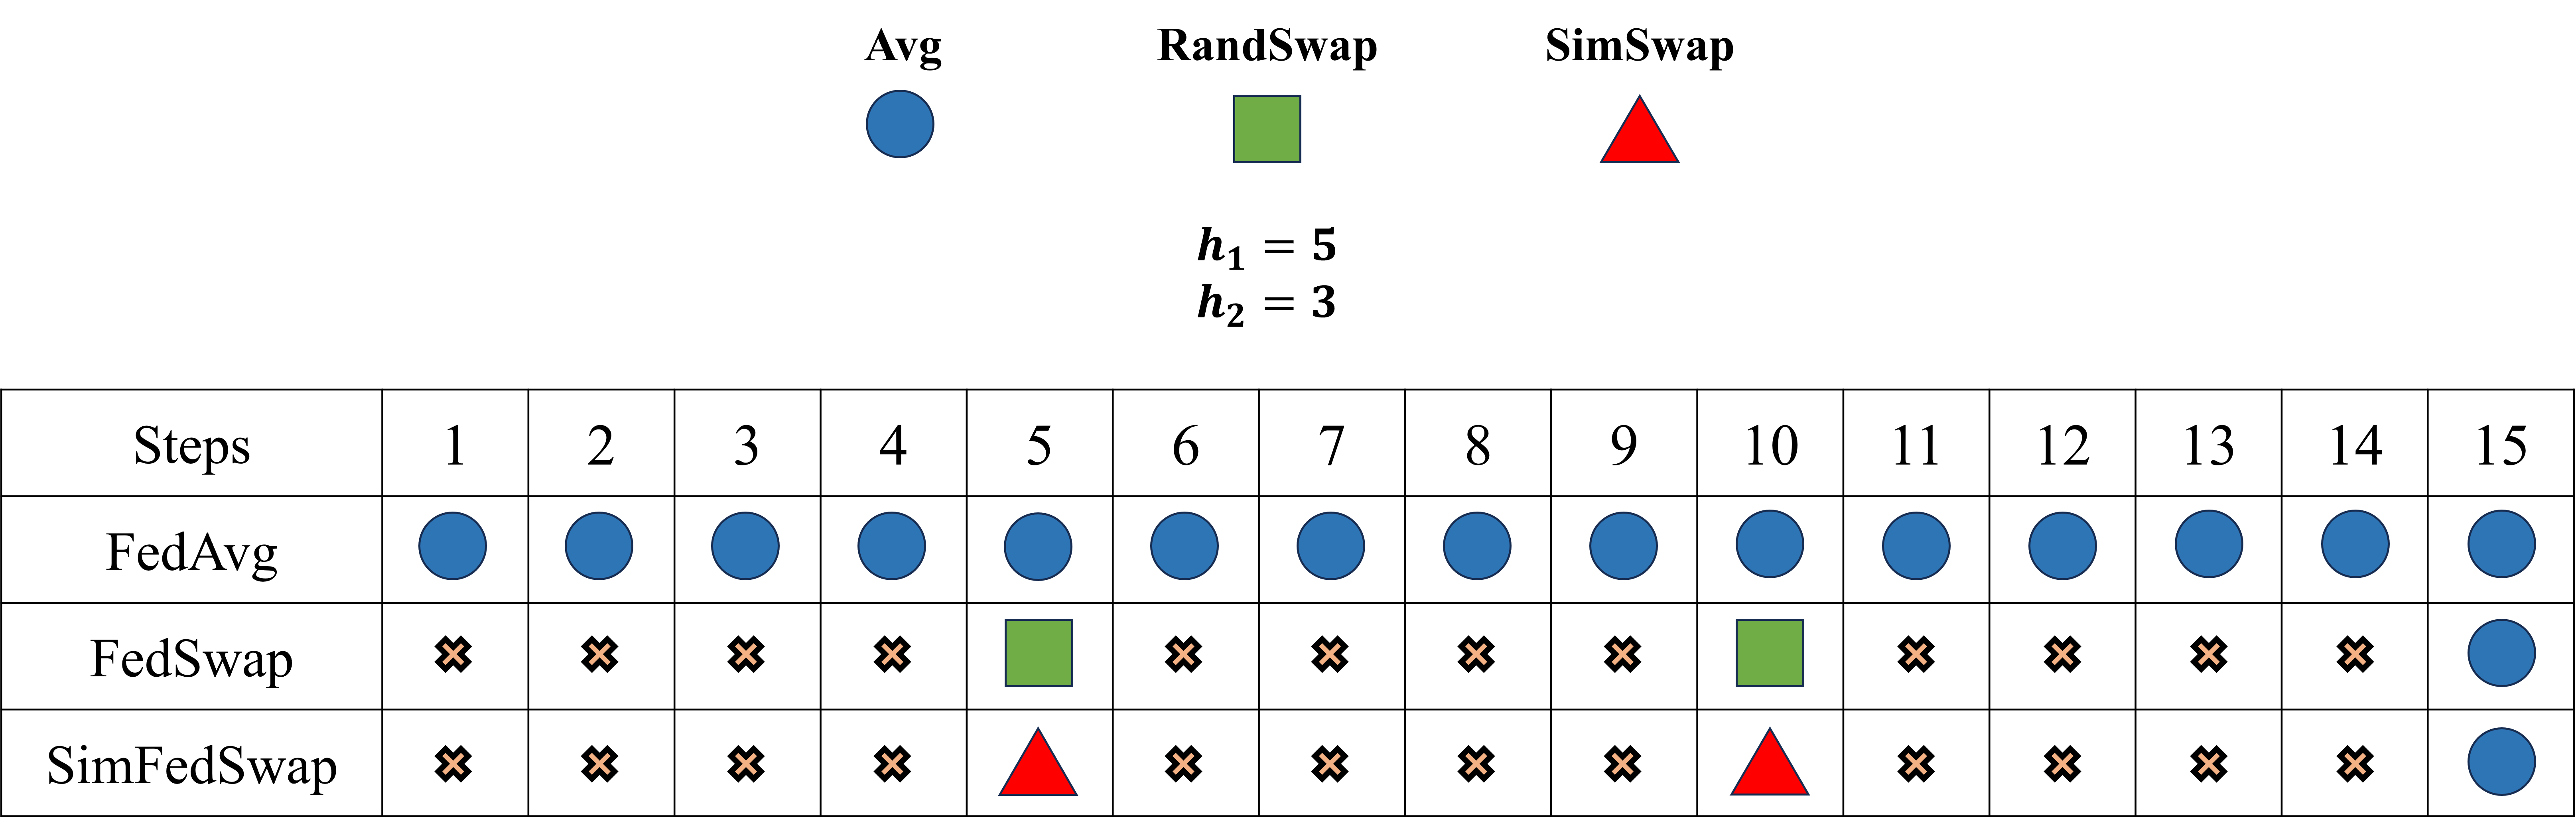
\includegraphics[scale=0.3]{images/chap4/compare_swap_net_traffic.png}%
	\caption{%
		تأثیر نحوه جابه‌جایی مدل‌ها بر ترافیک شبکه.
	}
	\label{compare_swap_net_traffic}
	\centering
\end{figure}
به‌طور خاص، در شبیه‌سازی‌هایی که پارامترهای \(h_1\) برابر با 5 و \(h_2\) برابر با 3 در نظر گرفته شده‌اند، روش \lr{FedSwap} موفق به کاهش
۸۶٫۶۶
درصدی هزینه‌های شبکه شده است. همچنین، روش \lr{SimFedSwap} توانسته این هزینه‌ها را تا ۸۰ درصد کاهش دهد. 


\subsection{
	تاثیر جابجایی مدل‌ها بر حریم شخصی در ارتباط بین سرور و کاربران
}
در روش یادگیری فدرال سنتی، مانند
\lr{FedAvg}%
، مدل‌ها پس از آموزش محلی توسط کاربران، به سرور مرکزی ارسال می‌شوند. سرور وظیفه تجمیع این مدل‌ها را بر عهده دارد و سپس مدل به‌روزرسانی‌ شده را به کاربران بازمی‌گرداند. در این روش، تعاملات فقط بین سرور و کاربران صورت می‌گیرد و هیچ ارتباط مستقیمی بین کاربران وجود ندارد. این امر باعث می‌شود که حریم شخصی کاربران به دلیل عدم تبادل مستقیم اطلاعات با یکدیگر، تا حد زیادی حفظ شود. همچنین کاربران نیازی به اعتماد به یکدیگر ندارند و تنها باید به سرور مرکزی اعتماد کنند.

در مقابل، در روش‌هایی که مدل‌ها بین خود کاربران جابه‌جا می‌شود، چه با واسطه سرور و چه بدون واسطه آن، خطرات بیشتری برای حریم شخصی وجود دارد. زمانی که مدل‌ها مستقیماً بین کاربران مبادله می‌شود، احتمال این که یکی از کاربران بتواند از طریق تحلیل مدل دریافت ‌شده اطلاعاتی در مورد داده‌های دیگر کاربران به دست آورد، افزایش می‌یابد. حتی اگر سرور به عنوان واسطه در این جابجایی‌ها عمل کند، همچنان خطراتی وجود خواهد داشت، زیرا سرور می‌تواند نقش ناظر را داشته باشد و از جابجایی مدل‌ها بین کاربران سوء استفاده کند. بنابراین، در هر دو حالت، جابجایی مدل‌ها بین کاربران نسبت به
\lr{FedAvg}
با چالش‌های بیشتری در زمینه حفظ حریم شخصی مواجه است.

در نتیجه، در روش
\lr{FedAvg}%
، به دلیل عدم ارتباط مستقیم بین کاربران، حریم شخصی به شکل بهتری حفظ می‌شود و تنها سرور مرکزی باید ایمن باشد. اما در روش جابجایی مدل‌ها بین کاربران، خطر نشت اطلاعات بین کاربران افزایش می‌یابد و این روش به پروتکل‌های امنیتی پیچیده‌تر و اعتماد بیشتر بین کاربران نیاز دارد.


\subsection{
	تاثیر جابجایی مدل‌ها بر حریم شخصی با توجه به واسطه بودن سرور
}
روش حریم خصوصی تفاضلی که در
\ref{privacy_challenge}
نیز به آن اشاره شد یکی از تکنیک‌های موثر برای حفظ حریم شخصی است که با اضافه کردن نویز به داده‌ها یا مدل‌ها، مانع از افشای اطلاعات حساس فردی می‌شود. این روش تضمین می‌کند که خروجی یک الگوریتم یادگیری به اندازه کافی تصادفی است، به‌طوری‌که حضور یا عدم حضور یک نمونه داده خاص در مجموعه داده‌ها، تاثیری بر خروجی نهایی نداشته باشد.

حال اگر از این روش در جابجایی مدل‌ها بین کاربران استفاده شود، تفاوت‌هایی بین دو رویکرد با واسطه سرور و بدون واسطه سرور وجود خواهد داشت. در حالتی که سرور واسطه باشد، اعمال حریم خصوصی تفاضلی می‌تواند به کنترل و مدیریت نویز اضافه شده کمک کند و سرور می‌تواند نقش فعالی در تضمین این که مدل‌ها به درستی ناشناس‌ شده‌اند، ایفا کند. این امر باعث می‌شود که خطر نشت اطلاعات به دلیل واسطه‌گری سرور کاهش یابد. اما همچنان باید به سرور اعتماد کرد که این فرآیند را به درستی انجام دهد.

در رویکرد بدون واسطه سرور، اعمال حریم خصوصی تفاضلی چالش‌برانگیزتر است، زیرا کاربران به‌طور مستقل باید نویز لازم را به مدل‌های خود اضافه کنند و در عین حال مطمئن شوند که سطح مناسبی از حفظ حریم شخصی برقرار است. در این حالت، هرگونه خطا یا ناهماهنگی در اعمال حریم خصوصی تفاضلی ممکن است منجر به افشای اطلاعات حساس شود. همچنین، نبود یک ناظر مرکزی مانند سرور، کار را برای هماهنگی و اجرای صحیح این روش پیچیده‌تر می‌کند.

در نتیجه، در صورت استفاده از روش حریم خصوصی تفاضلی، رویکرد با واسطه سرور به دلیل نظارت و کنترل متمرکز، از لحاظ حفظ حریم شخصی مزیت بیشتری دارد. در مقابل، در رویکرد بدون واسطه سرور، چالش‌های بیشتری برای کاربران وجود دارد که می‌تواند منجر به کاهش اثربخشی حریم خصوصی تفاضلی شود. در نهایت، اعتماد به سرور و هماهنگی دقیق بین کاربران نقش کلیدی در تعیین سطح امنیت و حریم شخصی خواهد داشت.




\section{
	نحوه تعیین کاربران نهایی جهت جابه‌جایی مدل‌ها در روش
	\lr{\texttt{\fontspec{Times New Roman} SimFedSwap}}
}
زمانی که همه مدل‌های شبکه عصبی در سرور مرکزی قرار دارند، وظیفه سرور این است که تصمیم بگیرد کدام کاربران مدل‌های خود را با یکدیگر جابه‌جا کنند. برای انجام این کار، ابتدا باید مدل‌ها با یکدیگر مقایسه شوند تا میزان شباهت بین آن‌ها مشخص شود. سپس، بر اساس این شباهت‌ها تعیین می‌شود که کدام کاربران مدل‌های شبکه عصبی خود را با یکدیگر مبادله کنند، یا به عبارت دیگر، سرور مشخص می‌کند کدام مدل به کدام کاربر ارسال شود.

نکته مهمی که باید مد نظر قرار داد این است که فرآیند بررسی شباهت بین مدل‌های شبکه عصبی ممکن است زمان‌بر باشد. بنابراین، برای تصمیم‌گیری سریع درباره جابه‌جایی مدل‌ها، باید از روش‌های مؤثری استفاده شود. در ادامه، دو روش برای تعیین کاربران نهایی جهت جابه‌جایی مدل‌ها معرفی می‌شود.


\subsection{
	روش جابه‌جایی حریصانه%
	\LTRfootnote{Greedy Swapping}
	\lr{\texttt{\fontspec{Times New Roman} (GS)}}
}\label{greedy_swapping}
در روش حریصانه، از بین تمام کاربران موجود، یک کاربر به‌صورت تصادفی انتخاب می‌شود. سپس مدل شبکه عصبی این کاربر با مدل‌های تمامی کاربران دیگر مقایسه می‌شود تا میزان شباهت آن‌ها سنجیده شود. در این مرحله، کاربری که مدل شبکه عصبی او کمترین شباهت را با مدل کاربر انتخاب‌ شده دارد، به عنوان کاربر مقصد برای جابه‌جایی مدل انتخاب می‌شود. پس از این انتخاب، سرور مدل‌های این دو کاربر را با یکدیگر جابه‌جا می‌کند و در نهایت این دو کاربر را از لیست انتخاب حذف خواهد کرد.

پس از انجام این جابه‌جایی، فرایند مشابهی برای کاربران باقی‌مانده تکرار می‌شود. ابتدا یک کاربر دیگر به‌صورت تصادفی انتخاب می‌شود و دقیقا همان روند بالا برای آن تکرار خواهد شد.
شبه کد کامل این روش در الگوریتم
\ref{algo_greedy_swapping}
ارائه شده است. علاوه بر این، نمادهای مختص به این الگوریتم در جدول
\ref{tabel_GreedySwappingNotations}
و همچنین تمامی نمادهای پایه در جدول
\ref{tabel_FedAvgNotations}
توضیح داده شده‌اند.
هدف از این جداول، فراهم کردن درکی جامع از نحوه عملکرد و پیاده‌سازی الگوریتم می‌باشد.


\begin{LTR}
	\SetAlgoNlRelativeSize{-1}
	\begin{algorithm}[t]
		\begin{RTL}
			\caption{%
				جابه‌جایی حریصانه
				\lr{(Greedy Swapping)}
			}
			\label{algo_greedy_swapping}
		\end{RTL}
		
		\begin{latin}
			\SetKwFunction{GreedySwapping}{GreedySwapping}
			\SetKwProg{Fn}{Function}{:}{end}
			\Fn{\GreedySwapping{}}{
				$LRS$ = copy of $U_t$\;
				$NS$ = (length of $U_t$ // 2) * $SP$\;
				\BlankLine
				
				\For{$NS$ times}{
					$RandomIndex$ = random integer between $0$ and length of $LRS$\;
					$SCB = LRS[RandomIndex]$\;
					remove $SCB$ from $LRS$\;
					
					\BlankLine
					Initialize $LstSimilarity$ as an empty list\;
					\For{each $RC \in LRS$}{
						$Sim = \texttt{ModelSimilarity} (w^{SCB}, w^{RC})$\;
						Append $Sim$ to $LstSimilarity$\;
					}
					$MinSimilarityIndex$ = index of the minimum value in $LstSimilarity$\;
					$SCD = LRS[MinSimilarityIndex]$\;
					remove $SCD$ from $LRS$\;
					\BlankLine
					
					$\texttt{Swap}(SCB, SCD)$\;
				}
			}
		\end{latin}
	\end{algorithm}
\end{LTR}


\begin{table}[h]
	\centering
	\caption{نمادهای مختص الگوریتم جابه‌جایی حریصانه}
	\label{tabel_GreedySwappingNotations}
	\begin{tabular}{cr}
		\hline
		متغیر & توضیحات \\
		\hline
		$LRS \, (LstRemainSwap)$ & لیست باقی‌مانده جابه‌جایی \\
		$NS \, (NumSwaps)$ & تعداد جابه‌جایی‌ها \\
		$SP \, (SwapPercentage)$ & ضریب کنترلی برای تعداد جابه‌جایی‌ها \\
		$RandomIndex$ & شاخص تصادفی \\
		$SCB \, (SwapClientBase)$ & کاربر مبدا جابه‌جایی \\
		$LstSimilarity$ & لیست مشابهت \\
		$RC \, (RemainClient)$ & کاربر باقی‌مانده \\
		$Sim$ & معیار مشابهت بین دو مدل شبکه عصبی \\
		$SCD \, (SwapClientDest)$ & کاربر مقصد جابه‌جایی
	\end{tabular}
\end{table}



در ادامه این مورد بررسی خواهد شد که تابع
\lr{ModelSimilarity}
در الگوریتم
\ref{algo_greedy_swapping}
چند مرتبه اجرا می‌شود. 
برای ساده‌تر کردن موضوع و فهم بهتر آن، لیست ‎\(LRS\) با \( n \) مقدار اولیه در نظر گرفته می‌شود (لیستی با \( n \) عضو) و همچنین مقدار \( NS \) برابر \( n/2 \) لحاظ خواهد شد. دلیل این انتخاب این است که با انجام \( n/2 \) جابه‌جایی، همه مدل‌ها یک بار جابه‌جا می‌شوند.
سپس حلقه اصلی به تعداد \( NS \) تکرار می‌شود. در هر تکرار از این حلقه یک عنصر تصادفی از \( LRS \) انتخاب و حذف خواهد شد. سپس برای هر عنصر باقی‌مانده در \( LRS \)، تابع
\lr{ModelSimilarity}
فراخوانی می‌شود.

تعداد تکرارهای حلقه داخلی که در آن تابع
\lr{ModelSimilarity}
فراخوانی می‌شود وابسته به تعداد عناصر باقی‌مانده در \( LRS \) است. به‌طور دقیق‌تر، در اولین تکرار حلقه اصلی، \( LRS \) شامل \(n-1\) عنصر است و در دومین تکرار، \( LRS \) شامل \(n-3\) عنصر خواهد بود; زیرا در هر تکرار از حلقه اصلی، یک عنصر به‌صورت تصادفی و یک عنصر دیگر با کمترین شباهت حذف می‌شوند.

به این ترتیب، تعداد کل فراخوانی‌های تابع
\lr{ModelSimilarity}
برابر است با مجموع تعداد عناصر باقی‌مانده در هر تکرار از حلقه اصلی:
\begin{equation}
	\sum_{i=0}^{NS-1} (n-1-2i)
\end{equation}
که این مجموع برای \( NS=n/2 \) به‌صورت زیر است:
\begin{equation}
	\sum_{i=0}^{(n/2)-1} (n-1-2i)
\end{equation}
این یک دنباله حسابی با مقدار اولیه \(a=n-1\) و قدر نسبت
 \(d=-2\) 
است و تعداد جملات آن برابر با \( NS \) است.
مجموع این دنباله حسابی به‌صورت زیر محاسبه می‌شود:
\begin{equation}
	S = NS \times \left( \frac{a+l}{2} \right)
\end{equation}
که در آن \( l \) مقدار آخرین جمله است و به این شکل به دست می‌آید:
\begin{equation}
	\begin{align*} 
		l &= n-1-2(NS-1) \\
		  &= n-1-2(n/2-1) \\
		  &= n-1-n+2 \\
		  &= 1
	\end{align*}
\end{equation}
بنابراین مجموع نهایی به این صورت خواهد بود:
\begin{equation}
	\begin{align*} 
		S &= (n/2) \times \left( \frac{(n-1)+1}{2} \right) \\
		&= (n/2) \times \left( \frac{n}{2} \right) \\
		&= \frac{n^2}{4}
	\end{align*}
\end{equation}
پس در نهایت تابع
\lr{ModelSimilarity}
به تعداد
\(
\floor{\frac{n^2}{4}}
 \) 
بار اجرا می‌شود.


\subsection{
مرتبه زمانی روش جابه‌جایی حریصانه
}\label{order_GS}
بر اساس فرضیات مطرح شده در بخش قبل، زمان اجرای الگوریتم جابه‌جایی حریصانه معادل \( O(kn^2) \) است.
باید توجه داشت که هنگام محاسبه مرتبه زمانی، مدت زمان اجرای تابع \lr{ModelSimilarity} برابر \( k \) در نظر گرفته شده است. این مقدار به معیار شباهتی که برای این تابع انتخاب می‌شود بستگی دارد و با توجه به نوع معیار، می‌تواند کاملا متفاوت باشد.


همچنین با توجه به این‌که مقدار \( NS \) برابر با \( n/2 \) فرض شده و هر بار اجرای حلقه اصلی شامل یک حذف از لیست \( LRS \) می‌شود که زمان اجرای آن \( O(n) \) است و با در نظر گرفتن این‌که حلقه داخلی نیز، طبق بررسی‌های انجام‌شده در بخش
\ref{greedy_swapping}،
مرتبه زمانی \( O(n) \) دارد، می‌توان نتیجه گرفت که ترکیب این دو عامل موجب می‌شود که کل زمان اجرای الگوریتم برابر با \( O(kn^2) \) باشد.
البته نکته مهم این است که محاسبات حلقه دوم می‌توانند به‌طور کامل به‌صورت موازی انجام شوند. به‌طور دقیق‌تر، عناصر موجود در لیست 
\lr{$LstSimilarity$} 
به یکدیگر وابستگی ندارند و می‌توان تمام آن‌ها را به‌طور همزمان محاسبه کرد. اگر سرور قابلیت اجرای موازی این عملیات را داشته باشد، محاسبه حلقه داخلی عملاً لحاظ نمی‌شود و مرتبه زمانی برابر
\( O(kn) \) 
خواهد شد. 


در نهایت، میزان مصرف حافظه توسط لیست
 \lr{$LstSimilarity$} 
در الگوریتم
 \ref{algo_greedy_swapping} 
بررسی می‌شود. همان‌طور که در بخش قبل توضیح داده شد، حلقه داخلی این الگوریتم در بیشترین حالت به تعداد \(n-1\) مرتبه اجرا می‌شود. بنابراین، از نظر حافظه، لیست
 \lr{$LstSimilarity$} 
در مرتبه \(O(n)\) قرار دارد. با این حال، باید توجه داشت که برای یافتن کمترین مقدار در یک مجموعه، حافظه‌ای به میزان \(O(1)\) نیز کافی است. 

در این الگوریتم، استفاده از لیست
 \lr{$LstSimilarity$} 
به منظور افزایش خوانایی و سادگی کد صورت گرفته است، اگرچه از لحاظ بهینه‌سازی حافظه می‌توان از روش‌های کم‌حافظه‌تری نیز استفاده کرد. به بیان دیگر، به‌جای نگهداری همه شباهت‌ها در یک لیست و سپس پیدا کردن کمترین مقدار، می‌توان به‌صورت مستقیم در همان حلقه داخلی کمترین شباهت را دنبال کرد و در هر تکرار، فقط مقدار کمینه فعلی را به‌روزرسانی کرد. این روش نیاز به حافظه کمتری دارد و با حافظه \(O(1)\) قابل انجام است.

با این حال، استفاده از لیست
 \lr{$LstSimilarity$} 
در این‌جا به منظور ساده‌تر و قابل فهم‌تر کردن کد انجام شده است. این انتخاب به توسعه‌دهندگان امکان می‌دهد تا الگوریتم را بهتر درک کنند و روند مقایسه شباهت‌ها را به وضوح مشاهده کنند، با این شرط که بهینه‌سازی حافظه در اولویت نباشد.




\subsection{
	روش جابه‌جایی حداقل شباهت%
	\LTRfootnote{Minimum Similarity Swapping}
	\lr{\texttt{\fontspec{Times New Roman} (MSS)}}
}
در این روش، برای این که حداقل شباهت ممکن بین تمامی مدل‌های شبکه عصبی به دست آید، لازم است تمامی مدل‌ها با یکدیگر مقایسه شوند و دو مدلی که کمترین شباهت را دارند با هم جابه‌جا شوند. به عنوان مثال، اگر \( n \) مدل وجود داشته باشد، باید یک ماتریس \( n \times n \) برای بررسی میزان شباهت‌ها ایجاد شود. در این ماتریس، شباهت مدل 1 با مدل 2 برابر با شباهت مدل 2 با مدل 1 در نظر گرفته می‌شود. همچنین به دلیل این که مقایسه یک مدل با خودش بی‌معنی است، ماتریس نهایی به شکل یک ماتریس بالا مثلثی%
\LTRfootnote{Upper Triangular Matrix}
(بدون قطر اصلی) تبدیل می‌شود. به این صورت که تنها حدود نیمی از ماتریس، شامل شباهت‌های مورد نیاز برای مقایسه است. در نتیجه ماتریس مورد نظر به شکل زیر در خواهد آمد.
\begin{equation}
	\begin{bmatrix}
		\infty & a^{12} & a^{13} & \cdots & a^{1n} \\
		\infty & \infty & a^{23} & \cdots & a^{2n} \\
		\infty & \infty & \infty & \cdots & a^{3n} \\
		\vdots & \vdots & \vdots & \ddots & \vdots \\
		\infty & \infty & \infty & \cdots & \infty
	\end{bmatrix}
	\label{eq_similarity_matrix}
\end{equation}

ابتدا، تمامی شباهت‌ها بین مدل‌ها محاسبه می‌شود و سپس از ماتریس ایجاد شده، کمترین مقدار شباهت انتخاب می‌شود. شماره سطر و ستون متناظر با این مقدار نشان می‌دهد که این دو مدل باید با یکدیگر جابه‌جا شوند. پس از انجام این جابه‌جایی، تمامی مقدارهای مربوط به سطر و ستون متناظر با این دو مدل باید به بی‌نهایت تغییر داده شوند تا در مراحل بعدی مجدد انتخاب نشوند. همچنین باید دقت کرد که هر دو سطر و ستون مرتبط با این دو مدل باید به بی‌نهایت تغییر داده شوند.

برای درک بهتر، فرض کنید کمترین مقدار شباهت در سطر سوم و ستون ششم ماتریس قرار دارد. در این حالت، مدل‌های سوم و ششم باید با یکدیگر جابه‌جا شوند. پس از این جابه‌جایی، لازم است که تمامی مقادیر در سطرهای سوم و ششم و همچنین ستون‌های سوم و ششم به بی‌نهایت تغییر کنند تا این دو مدل دیگر مورد بررسی قرار نگیرند. به این ترتیب، در دور بعدی، کوچک‌ترین مقدار شباهت از ماتریس انتخاب می‌شود و چون مقادیر مربوط به مدل‌های سوم و ششم به بی‌نهایت تغییر کرده‌اند، دیگر در این مرحله حضور نخواهند داشت و انتخاب نمی‌شوند. شبه کد کامل این روش در الگوریتم
\ref{algo_min_similarity_swapping}
ارائه شده است. علاوه بر این، نمادهای مختص به این الگوریتم در جدول
\ref{tabel_MinSimilaritySwapNotations}
توضیح داده شده‌اند.


\begin{LTR}
	\SetAlgoNlRelativeSize{-1}
	\begin{algorithm}[t]
		\begin{RTL}
			\caption{%
				جابه‌جایی حداقل شباهت
				\lr{(Minimum Similarity Swapping)}
			}
			\label{algo_min_similarity_swapping}
		\end{RTL}
		
		\begin{latin}
			\SetKwFunction{MinSimilaritySwapping}{MinSimilaritySwapping}
			\SetKwProg{Fn}{Function}{:}{end}
			\Fn{\MinSimilaritySwapping{}}{
				Initialize $SimArray$\;
				$L$ = length of $U_t$\;
				\BlankLine
				
				\For{each $row$ from $0$ to $L$}{
					\For{each $col$ from $(row+1)$ to $L$}{
						$Sim = \texttt{ModelSimilarity} (w^{row}, w^{col})$\;
						Append $Sim$ to $SimArray$\;
					}
				}
				\BlankLine
				
				$NS$ = ($L$ // 2) * $SP$\;
				\For{$NS$ times}{
					$MI$ = index of minimum value in $SimArray$\;
					$row, col$ = find $row$ and $col$ number, based on $MI$\;					
					Set all values of $SimArray[row, col]$ to $\infty$\;
					\BlankLine
					
					$\texttt{Swap}(w^{row}, w^{col})$\;
				}
			}
		\end{latin}
	\end{algorithm}
\end{LTR}



\begin{table}[h]
	\centering
	\caption{نمادهای مختص الگوریتم جابه‌جایی حداقل شباهت}
	\label{tabel_MinSimilaritySwapNotations}
	\begin{tabular}{cr}
		\hline
		متغیر & توضیحات \\
		\hline
		$SimArray$ & آرایه مشابهت \\
		$L$ & طول مجموعه‌ای از کاربران در گام $t$ \\
		$MI \, (MinIndex)$ & شاخص مقدار کمینه در آرایه مشابهت \\
		$row$ & شماره سطر بر اساس دید ماتریس مشابهت \\
		$col$ & شماره ستون بر اساس دید ماتریس مشابهت
	\end{tabular}
\end{table}




در این الگوریتم، تعداد دفعات اجرای تابع
\lr{ModelSimilarity}
به تعداد کل جابه‌جایی‌ها بین کاربران نهایی وابسته نیست. همان‌طور که در الگوریتم
\ref{algo_min_similarity_swapping}
مشاهده می‌شود، ماتریس شباهت تنها یک بار محاسبه خواهد شد. با توجه به ساختار ماتریس بالا مثلثی در رابطه
\ref{eq_similarity_matrix}
و با فرض این که تعداد مدل‌های کاربران برابر \(n\) در نظر گرفته شود، مقدار \(L\) در الگوریتم نیز برابر \(n\) خواهد شد.
در نتیجه، تعداد دفعات اجرای تابع
\lr{ModelSimilarity}
در الگوریتم جابه‌جایی حداقل شباهت، برابر با \(\frac{n(n-1)}{2}\) خواهد بود.


\subsection{
مرتبه زمانی و نحوه پیاده‌سازی روش جابه‌جایی حداقل شباهت
}
بر اساس فرضیات مطرح‌شده در بخش قبلی، زمان اجرای الگوریتم جابه‌جایی حداقل شباهت برابر با \( O(kn^2 + n^3) \) است. همچنین، مطابق با آنچه در بخش
\ref{order_GS}
بیان شد، مرتبه زمانی تابع
\lr{ModelSimilarity}
برابر
$k$
در نظر گرفته شده و طبق فرضیات بخش قبل، این تابع به تعداد \( O(n^2) \) بار اجرا می‌شود. بنابراین، بخش اول محاسبات با مرتبه زمانی \( O(kn^2) \) مشخص می‌شود.


برای محاسبات بخش دوم، پیدا کردن عنصر کمینه در ماتریس مشابهت، خود از مرتبه زمانی \(O(n^2)\) است. بنابراین، وقتی که حلقه اصلی \(n/2\) بار اجرا شود و هر بار نیاز به پیدا کردن عنصر کمینه در ماتریس مشابهت داشته باشد، مرتبه زمانی بخش دوم الگوریتم برابر \(O(n^2) \times O(n/2)\) خواهد بود که به \(O(n^3)\) ساده‌سازی می‌شود.
پس با ترکیب بخش اول و بخش دوم مرتبه زمانی کل الگوریتم برابر
\( O(kn^2 + n^3) \) 
خواهد شد.


لازم به ذکر است که محاسبات هر یک از عناصر ماتریس مشابهت، مستقل از یکدیگر هستند. اگر سرور قابلیت اجرای موازی این عملیات را داشته باشد، مرتبه زمانی محاسبه بخش اول برابر
\( O(k) \) 
و در نتیجه کل الگوریتم برابر با
\( O(k + n^3) \)
خواهد شد.


ماتریس مشابهت، در حالت عادی، دارای \(n^2\) عنصر است.
با بررسی دقیق‌تر الگوریتم و تعداد اجراهای حلقه دوم، در صورتی که از ماتریس مشابهت در پیاده‌سازی استفاده شود، از نظر زمان اجرا رابطه زیر به دست می‌آید:
\begin{equation}
	\begin{align*} 
		\left(\frac{n}{2}\right) \times (n^2 + 4n) &= \left(\frac{n^3}{2}\right)+2n^2 \\
		 &\xlongequal{\times 4} 2n^3 + 8n^2
	\end{align*}
\end{equation}
در این رابطه، تعداد اجراهای حلقه دوم برابر \(n/2\)، پیداکردن مقدار کمینه در ماتریس مشابهت برابر با \(n^2\) و انتساب مقدار بی‌نهایت برای دو سطر و ستون ماتریس مشابهت برابر با \(4n\) است.

با توجه به رابطه
\ref{eq_similarity_matrix}،
بیش از نصف ماتریس، شامل مقادیر بی‌نهایت می‌باشد. بنابراین، با پیاده‌سازی ماتریس به‌صورت یک آرایه یک‌بعدی و تنها ذخیره‌سازی مقادیر بالا مثلثی، می‌توان با انجام چند عملیات ساده ریاضی به مقدار سطر و ستون مورد نظر در ماتریس مشابهت دست یافت.

در این پیاده‌سازی، آرایه یک‌بعدی جدید دارای \(\frac{n(n-1)}{2}\) عنصر خواهد بود. اگر حلقه دوم الگوریتم، مجدد بررسی شود، زمان اجرای آن به‌صورت زیر خواهد بود:
\begin{equation}
	\begin{align*} 
		\left(\frac{n}{2}\right) \times \left(\frac{n(n-1)}{2} + 4n\right) &= \left(\frac{n^2(n-1)}{4} \right)+2n^2 \\
		&= \left(\frac{n^3}{4} - \frac{n^2}{4}\right) +2n^2 \\
		&\xlongequal{\times 4} n^3-n^2+8n^2 \\
		&= n^3+7n^2
	\end{align*}
\end{equation}
در این عبارت، تعداد اجراهای حلقه دوم برابر \(n/2\)، پیداکردن مقدار کمینه در آرایه برابر \(\frac{n(n-1)}{2}\) و در نهایت انتساب مقدار بی‌نهایت در آرایه مربوطه برابر با \(4n\) خواهد بود.

همان‌طور که مشاهده می‌شود، این پیاده‌سازی تقریبا سرعت اجرای الگوریتم را دو برابر می‌کند. اگرچه از نظر مرتبه زمانی بهبودی حاصل نشد، اما افزایش سرعت اجرا به میزان دو برابر، بهبود قابل توجهی در روند آموزش محسوب می‌شود. همچنین از نظر حافظه نیز بهبود حاصل شده است، زیرا در صورت استفاده از ماتریس مشابهت نیاز به ذخیره‌سازی \(n^2\) عنصر است، در حالی که با به‌کارگیری آرایه مشابهت تنها \(\frac{n(n-1)}{2}\) عنصر ذخیره خواهد شد. بنابراین، استفاده از ساختار آرایه یک بعدی می‌تواند بسیار مفید بوده و به کارایی الگوریتم کمک کند.




\section{جمع‌بندی}

روش جابه‌جایی فدرال به‌جای ادغام مدل‌های محلی در هر مرحله از یادگیری فدرال، این مدل‌ها را بین دستگاه‌ها جابه‌جا می‌کند. این روش با هدف کاهش تأثیرات منفی ناشی از داده‌های
\lr{non-IID}
و بهبود دقت مدل‌ها طراحی شده است. جابه‌جایی مدل‌ها به دستگاه‌های مختلف اجازه می‌دهد تا به داده‌های متنوع‌تری دسترسی پیدا کنند و عملکرد مدل سراسری بهبود یابد. همچنین، جابه‌جایی فدرال در دو حالت تصادفی و بر پایه شباهت معرفی شد که در حالت دوم، مدل‌هایی که کمترین شباهت را دارند جابه‌جا می‌شوند تا تنوع داده‌ها افزایش یابد و یادگیری بهینه‌تر صورت گیرد.


جابه‌جایی مدل‌ها در روش‌های
\lr{FedSwap}
و
\lr{SimFedSwap}
می‌تواند هزینه‌های ارتباطی را به میزان قابل‌توجهی کاهش دهد و از این نظر بر ترافیک شبکه تاثیر مثبتی داشته باشد. از سوی دیگر، این جابه‌جایی‌ها می‌توانند چالش‌های جدیدی را در زمینه حفظ حریم شخصی ایجاد کنند، به ویژه زمانی که مدل‌ها مستقیما بین کاربران جابه‌جا می‌شوند. استفاده از روش‌های حریم خصوصی تفاضلی می‌تواند به کاهش این خطرات کمک کند، اما اجرای صحیح آن‌ها، به ویژه بدون واسطه‌گری سرور، چالش ‌برانگیز است.


برای حفظ دقت در مقایسه‌های شبکه‌های عصبی در شرایط مختلف، لازم است شاخص‌های شباهت در برابر تغییرات مقاوم باشند. برای تحلیل عمیق‌تر، استفاده از روش‌های مختلفی مانند معیارهای نرمال‌شده یا همان
\lr{CKA}
پیشنهاد می‌شود. ارزیابی لایه‌های شبکه به‌صورت جداگانه و ترکیب نتایج آن‌ها به بهینه‌سازی شاخص انتخاب شده کمک می‌کند. در نهایت، در روش
\lr{SimFedSwap}%
، سرور دو مدل با کمترین شباهت را انتخاب و با یکدیگر جابه‌جا می‌کند که این فرآیند بر اساس روش حریصانه یا حداقل شباهت انجام می‌گیرد.


% Chapter 5
\chapter{پیاده‌سازی و بررسی نتایج}

\section{مقدمه}
تست


\section{انواع مجموعه داده}
در این پژوهش از انواع مجموعه داده‌ها برای بررسی و ارزیابی روش مورد نظر استفاده شده است. این مجموعه داده‌ها هر یک ویژگی‌های منحصر به فردی دارند که به تحلیل‌های دقیق‌تر و جامع‌تر کمک می‌کنند. در ادامه، هر یک از این مجموعه داده‌ها به طور مفصل معرفی و توضیح داده خواهد شد تا اهمیت و کاربردهای آن‌ها مشخص گردد.

\subsection{
مجموعه داده
	\lr{MNIST}%
	\LTRfootnote{Modified National Institute of Standards and Technology}
}
مجموعه داده
\lr{MNIST}
یکی از مشهورترین و پر استفاده‌ترین مجموعه داده‌ها در زمینه یادگیری ماشین است. این مجموعه شامل تصاویر دست‌نویس از اعداد 0 تا 9 می‌باشد و به طور گسترده‌ای برای آموزش و ارزیابی مدل‌های مختلف یادگیری ماشین به کار گرفته می‌شود.
مجموعه داده
\lr{MNIST}
در دهه 1990 توسط یان لکون%
\LTRfootnote{Yann LeCun}،
کورینا کورتس%
\LTRfootnote{Corinna Cortes}
و کریستوفر برجس%
\LTRfootnote{Christopher Burges}
 ایجاد شد. هدف اصلی این مجموعه داده، فراهم کردن یک مجموعه استاندارد برای ارزیابی الگوریتم‌های یادگیری ماشین و بینایی کامپیوتر بود.

مجموعه داده
\lr{MNIST}
شامل 70٬000 تصویر از ارقام دست‌نویس است که به دو بخش شامل مجموعه آموزش با 60٬000 تصویر و مجموعه تست با 10٬000 تصویر تقسیم می‌شود. هر تصویر دارای ابعاد
(28$\times$28)
پیکسل است که به صورت خاکستری%
\LTRfootnote{Grayscale}
ذخیره شده‌اند و هر پیکسل دارای مقداری بین 0 (سیاه) تا 255 (سفید) است. همچنین تمامی تصاویر با یک برچسب عددی بین 0 تا 9 همراه هستند که نمایانگر رقم موجود در تصویر می‌باشد
\cite{lecun1998gradient}.
چند نمونه از اعضای این مجموعه داده در شکل
\ref{mnist}%
، نمایش داده شده‌اند.

\begin{figure}[t]
	\centering
	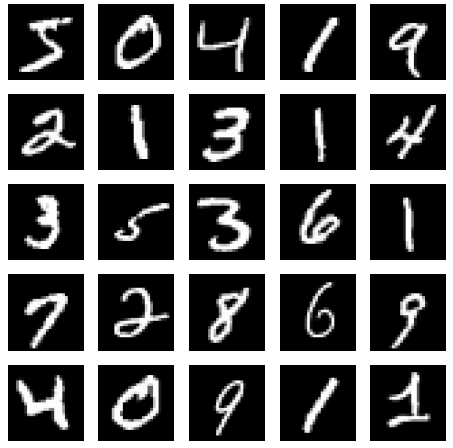
\includegraphics[scale=0.5]{images/chap5/mnist.png}%
	\caption{%
		چند نمونه از اعضای مجموعه داده
		\lr{MNIST}
		\cite{holzer2023dynamically}.
	}
	\label{mnist}
	\centering
\end{figure}


داده‌ها معمولاً در قالب دو فایل باینری شامل یکی برای تصاویر و دیگری برای برچسب‌ها ذخیره می‌شوند. هر تصویر به صورت یک بردار از اعداد بین 0 تا 255 با طول 784
(28$\times$28)
ذخیره می‌شود. به دلیل یکنواختی تصاویر و اندازه کوچک آن‌ها، نیاز به پیش‌پردازش پیچیده‌ای ندارند. یکی از مراحل پیش‌پردازش شامل نرمال‌سازی یا همان تبدیل مقادیر پیکسل‌ها به مقادیر بین 0 و 1 می‌باشد.

مجموعه داده
\lr{MNIST}
به عنوان یک نقطه شروع استاندارد برای آموزش و ارزیابی مدل‌های مختلف یادگیری عمیق و شبکه‌های عصبی استفاده می‌شود. محققان اغلب از
\lr{MNIST}
برای مقایسه کارایی الگوریتم‌های جدید با الگوریتم‌های موجود استفاده می‌کنند. این مجموعه شامل نمونه‌های متنوعی از ارقام دست‌نویس از افراد مختلف است که موجب می‌شود به عنوان یک معیار استاندارد برای مقایسه مدل‌ها و الگوریتم‌ها مورد استفاده قرار گیرد.

مجموعه داده
\lr{MNIST}
دارای مزایای زیادی از جمله سادگی، در دسترس بودن، استاندارد بودن و پراکندگی داده‌ها می‌باشد. با این حال، این مجموعه داده دارای معایبی نیز هست. به عنوان مثال، برای مسائل پیچیده‌تر و واقعی‌تر ممکن است
\lr{MNIST}
خیلی ساده باشد و نتواند چالش‌های واقعی را نشان دهد. همچنین، این مجموعه داده شامل تنها اعداد 0 تا 9 است و برای سایر کاربردهای دسته‌بندی تصویر ممکن است کافی نباشد.

کاربردهای عملی این مجموعه داده شامل آموزش شبکه‌های عصبی متفاوت برای بهبود دقت دسته‌بندی، تست و ارزیابی مدل‌های مختلف یادگیری عمیق و الگوریتم‌های بهینه‌سازی است. بسیاری از مدل‌ها و الگوریتم‌های پیشرفته امروزی با استفاده از مجموعه داده
\lr{MNIST}
توسعه و ارزیابی شده‌اند.

به طور کلی، مجموعه داده
\lr{MNIST}
با توجه به دلایل ذکر شده، یکی از مهم‌ترین و پراستفاده‌ترین مجموعه داده‌ها در زمینه یادگیری ماشین و بینایی کامپیوتر است. این مجموعه به محققان و دانشجویان کمک می‌کند تا مفاهیم پایه‌ای یادگیری ماشین را به خوبی درک کرده و الگوریتم‌های جدید را ارزیابی کنند.


\subsection{
	مجموعه داده
	\lr{CIFAR-10}%
	\LTRfootnote{Canadian Institute For Advanced Research}
}
مجموعه داده
\lr{CIFAR-10}
یکی از معروف‌ترین و پرکاربردترین مجموعه داده‌های مورد استفاده در حوزه یادگیری ماشین و بینایی کامپیوتر است. این مجموعه داده توسط گروهی به سرپرستی الکس کریژفسکی%
\LTRfootnote{Alex Krizhevsky}
و جفری هینتون%
\LTRfootnote{Geoffrey Hinton}
در دانشگاه تورنتو گردآوری شده و برای ارزیابی و آزمایش مدل‌های یادگیری عمیق به کار می‌رود.


مجموعه داده
\lr{CIFAR-10}
شامل 60٬000 تصویر رنگی با اندازه
32$\times$32
پیکسل است که به 10 کلاس مختلف تقسیم شده‌اند. هر کلاس شامل 6٬000 تصویر است که به صورت مساوی بین مجموعه‌های آموزشی و آزمایشی توزیع شده‌اند. این کلاس‌ها شامل مواردی مانند هواپیما، اتومبیل، پرنده، گربه، گوزن، سگ، قورباغه، اسب، کِشتی و کامیون هستند. هر یک از این کلاس‌ها دارای تصاویری است که تنوع بالایی از زوایا، پس‌زمینه‌ها و شرایط نوری مختلف را شامل می‌شود
\cite{krizhevsky2009learning}.
در شکل
\ref{cifar10}%
، چند نمونه از هر کلاس در مجموعه داده
\mbox{\lr{CIFAR-10}}
به نمایش در آمده است.


\begin{figure}[t]
	\centering
	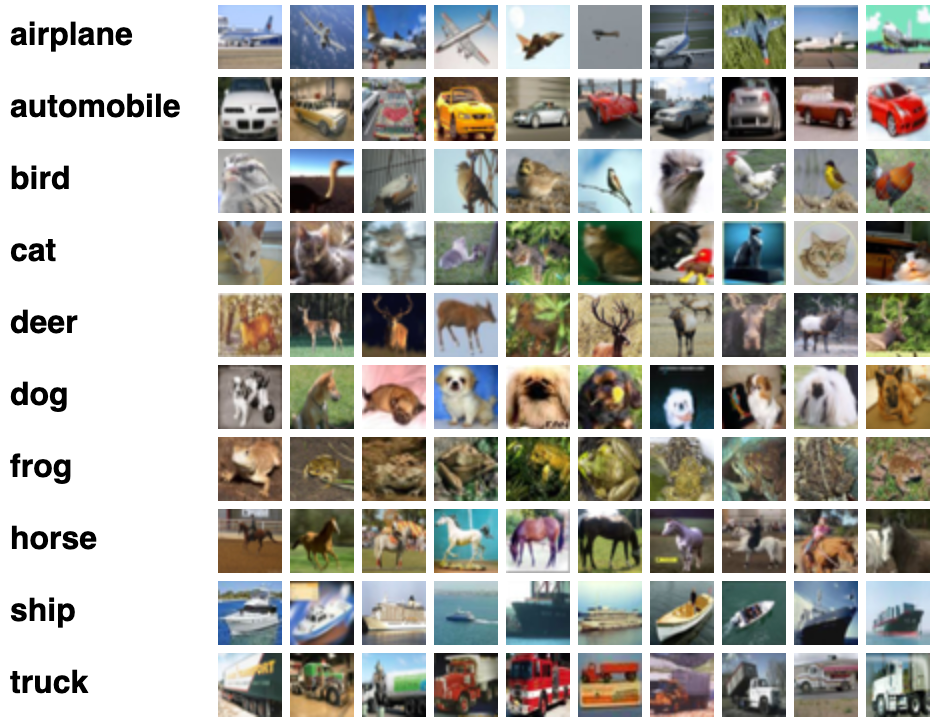
\includegraphics[scale=0.7]{images/chap5/cifar10.png}%
	\caption{%
		چند نمونه از هر کلاس در مجموعه داده
		\lr{CIFAR-10}
		\cite{Evan2022CIFAR10}.
	}
	\label{cifar10}
	\centering
\end{figure}



یکی از ویژگی‌های مهم مجموعه داده
\lr{CIFAR-10}
تنوع بالای تصاویر در هر کلاس است. این تنوع باعث می‌شود که مدل‌های یادگیری عمیق نیاز به توانایی تعمیم‌دهی بالا برای تشخیص صحیح کلاس‌ها داشته باشند. این مجموعه داده برای آموزش و ارزیابی مدل‌های مختلفی مورد استفاده قرار می‌گیرد و بسیاری از پژوهش‌ها و مقالات علمی از آن به عنوان مبنای مقایسه عملکرد مدل‌ها استفاده کرده‌اند.

مجموعه داده
\lr{CIFAR-10}
به دو بخش آموزشی و آزمایشی تقسیم شده است. بخش آموزشی شامل 50٬000 تصویر و بخش آزمایشی شامل 10٬000 تصویر است. این تقسیم‌بندی، استانداردی برای ارزیابی مدل‌ها فراهم می‌کند، به طوری که مدل‌ها می‌توانند بر روی مجموعه آموزشی، آموزش دیده و سپس بر روی مجموعه آزمایشی ارزیابی شوند. این روش به محققان امکان می‌دهد تا عملکرد مدل‌ها را به صورت عینی و قابل تکرار مقایسه کنند.

به دلیل اندازه کوچک تصاویر (%
32$\times$32
پیکسل)، پردازش و آموزش مدل‌ها بر روی
\lr{CIFAR-10}
نسبتاً سریع و کم هزینه است. این ویژگی باعث شده تا مجموعه داده 
\lr{CIFAR-10}
برای آزمایش مدل‌ها بسیار مناسب باشد. بسیاری از ابزارها و چارچوب‌های%
\LTRfootnote{Frameworks}
یادگیری ماشین مانند
\lr{PyTorch}
و
\lr{TensorFlow}
شامل توابع و ابزارهای آماده برای بارگذاری و استفاده از این مجموعه داده هستند که این امر نیز به سهولت استفاده از آن کمک می‌کند.

در نهایت، مجموعه داده
\lr{CIFAR-10}
با ارائه تصاویری متنوع و چالش‌برانگیز در کلاس‌های مختلف، ابزاری قدرتمند برای آموزش و ارزیابی مدل‌های یادگیری عمیق فراهم می‌کند. این مجموعه داده نه تنها در پژوهش‌های دانشگاهی بلکه در صنعت نیز به عنوان معیاری برای ارزیابی پیشرفت‌ها در حوزه بینایی کامپیوتر استفاده می‌شود.


\subsection{
	مجموعه داده
	\lr{CINIC-10}%
	\LTRfootnote{CIFAR-10 and ImageNet Combined}
}
مجموعه داده
\lr{CINIC-10}
یک مجموعه داده تصویری گسترده و متنوع است که برای ارزیابی عملکرد مدل‌های یادگیری ماشین به ویژه در زمینه‌های مرتبط با طبقه‌بندی تصاویر مورد استفاده قرار می‌گیرد. این مجموعه داده ترکیبی از تصاویر موجود در مجموعه‌ داده‌های معروف
\lr{CIFAR-10}
و
\lr{ImageNet}
است. این ترکیب به منظور ایجاد مجموعه‌ای گسترده‌تر و متنوع‌تر از تصاویر انجام شده است که می‌تواند به ارزیابی دقیق‌تر و واقع‌گرایانه‌تر مدل‌ها کمک کند.

مجموعه داده
\lr{CINIC-10}
شامل 270٬000 تصویر است که در 10 کلاس مختلف دسته‌بندی شده‌اند. هر کلاس شامل 27٬000 تصویر است که به دو بخش آموزشی و آزمایشی تقسیم شده‌اند. بخش آموزشی شامل 180٬000 تصویر و بخش آزمایشی شامل 90٬000 تصویر است. این تقسیم‌بندی منظم به محققان و مهندسان یادگیری ماشین این امکان را می‌دهد که به راحتی مدل‌های خود را آموزش داده، اعتبارسنجی و آزمایش کنند.

تصاویر موجود در
\lr{CINIC-10}
دارای ابعاد
32$\times$32
پیکسل هستند که مشابه ابعاد تصاویر موجود در مجموعه داده
\lr{CIFAR-10}
است. این ویژگی باعث می‌شود که مدل‌های از پیش آموزش دیده بر روی
\lr{CIFAR-10}
بتوانند به راحتی بر روی این مجموعه داده نیز مورد استفاده قرار گیرند و ارزیابی شوند. با این حال، تنوع بیشتر تصاویر در
\lr{CINIC-10}
نسبت به
\lr{CIFAR-10}
به دلیل ترکیب تصاویر از
\lr{ImageNet}،
چالشی جدی‌تر برای مدل‌های یادگیری ماشین فراهم می‌کند
\cite{darlow2018cinic}.
در شکل
\ref{cinic10}%
، تعدادی نمونه از کلاس خودرو در مجموعه داده
\mbox{\lr{CIFAR-10}}
به نمایش در آمده است.


\begin{figure}[b!]
	\centering
	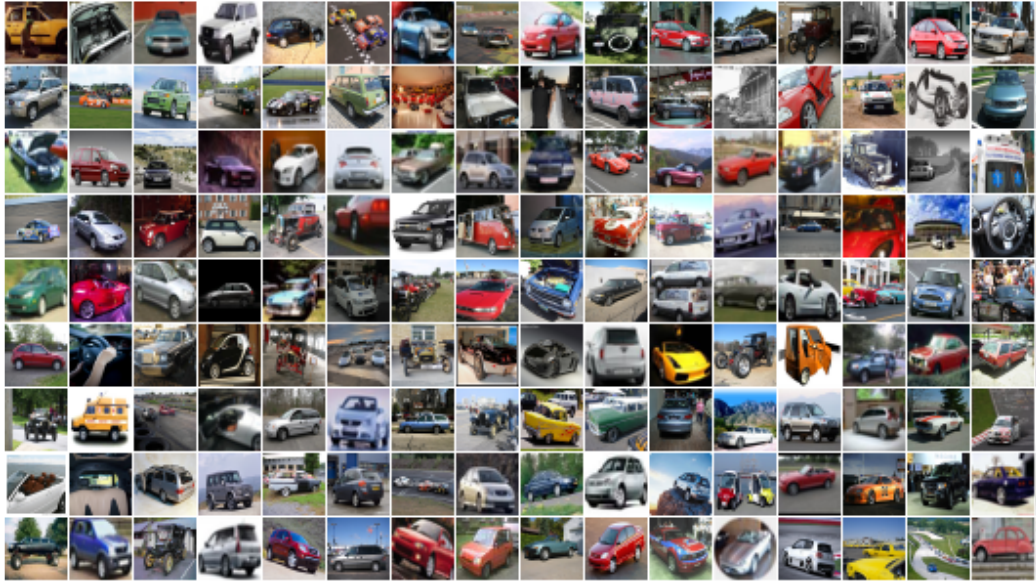
\includegraphics[scale=0.5]{images/chap5/cinic10.png}%
	\caption{%
		تعدادی نمونه از کلاس خودرو در مجموعه داده
		\lr{CINIC-10}
		\cite{darlow2018cinic}.
	}
	\label{cinic10}
	\centering
\end{figure}



یکی از اهداف اصلی ایجاد
\lr{CINIC-10}،
افزایش تنوع و پیچیدگی تصاویر مورد استفاده برای آموزش و ارزیابی مدل‌ها بود. این مجموعه داده شامل تصاویری از دنیای واقعی است که در شرایط نوری مختلف و با پس‌زمینه‌های متنوع گرفته شده‌اند. این ویژگی به مدل‌ها کمک می‌کند تا به جای اینکه تنها بر روی مجموعه‌ای محدود از تصاویر آموزش ببینند، توانایی تعمیم‌دهی خود را به تصاویر جدید و غیرمنتظره نیز افزایش دهند.

در نهایت،
\lr{CINIC-10}
با هدف ارتقای استانداردهای ارزیابی مدل‌های یادگیری عمیق و بهبود عملکرد آن‌ها در مواجهه با داده‌های واقعی و متنوع ایجاد شده است. این مجموعه داده به محققان این امکان را می‌دهد که مدل‌های خود را در شرایط نزدیک به دنیای واقعی آزمایش کرده و نقاط ضعف و قوت آن‌ها را بهتر شناسایی کنند. به همین دلیل،
\lr{CINIC-10}
به عنوان یک ابزار ارزشمند در جامعه یادگیری ماشین شناخته می‌شود و به طور گسترده‌ای مورد استفاده قرار می‌گیرد.


\subsection{
	مجموعه داده
	\lr{FEMNIST}%
	\LTRfootnote{Federated Extended MNIST}
}
مجموعه داده
\lr{FEMNIST}
یک مجموعه داده توسعه‌یافته از مجموعه مشهور
\lr{MNIST}
است که برای کاربردهای یادگیری فدرال طراحی شده است.
این مجموعه داده شامل 814٬255 تصویر است که در 62 کلاس مختلف دسته‌بندی شده‌اند و 10 درصد این داده‌ها به بخش آموزشی تعلق دارند. مجموعه داده
\lr{FEMNIST}
از تصاویر دست‌نوشته به وجود آمده است که شامل اعداد و حروف الفبای انگلیسی می‌شود.

برخلاف مجموعه داده
\lr{MNIST}
که تنها شامل اعداد دست‌نوشته از صفر تا نه است، مجموعه داده
\lr{FEMNIST}
شامل حروف بزرگ و کوچک الفبای انگلیسی نیز می‌باشد. این ویژگی باعث می‌شود که
\lr{FEMNIST}
نسبت به
\lr{MNIST}
تنوع بیشتری داشته باشد و برای آزمایش مدل‌های پیچیده‌، مناسب‌تر باشد
\cite{caldas2018leaf}.
چند نمونه از اعضای این مجموعه داده در شکل
\ref{femnist}%
، نمایش داده شده‌اند.
در این مجموعه داده، تعداد داده‌ها در هر کلاس یکسان نیست و کلاس‌های مختلف دارای مقادیر متفاوتی از داده‌ها هستند. شکل
\ref{count_all_classes}%
، تعداد داده‌های هر کلاس و نحوه نام‌گذاری آن‌ها را نشان می‌دهد.


\begin{figure}[b!]
	\centering
	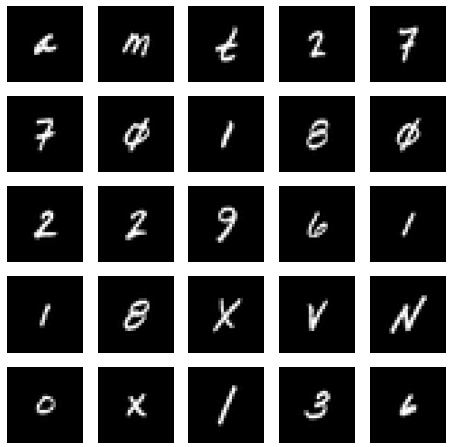
\includegraphics[scale=0.5]{images/chap5/femnist.png}%
	\caption{%
		چند نمونه از اعضای مجموعه داده
		\lr{FEMNIST}
		\cite{holzer2023dynamically}.
	}
	\label{femnist}
	\centering
\end{figure}


\begin{figure}[t]
	\centering
	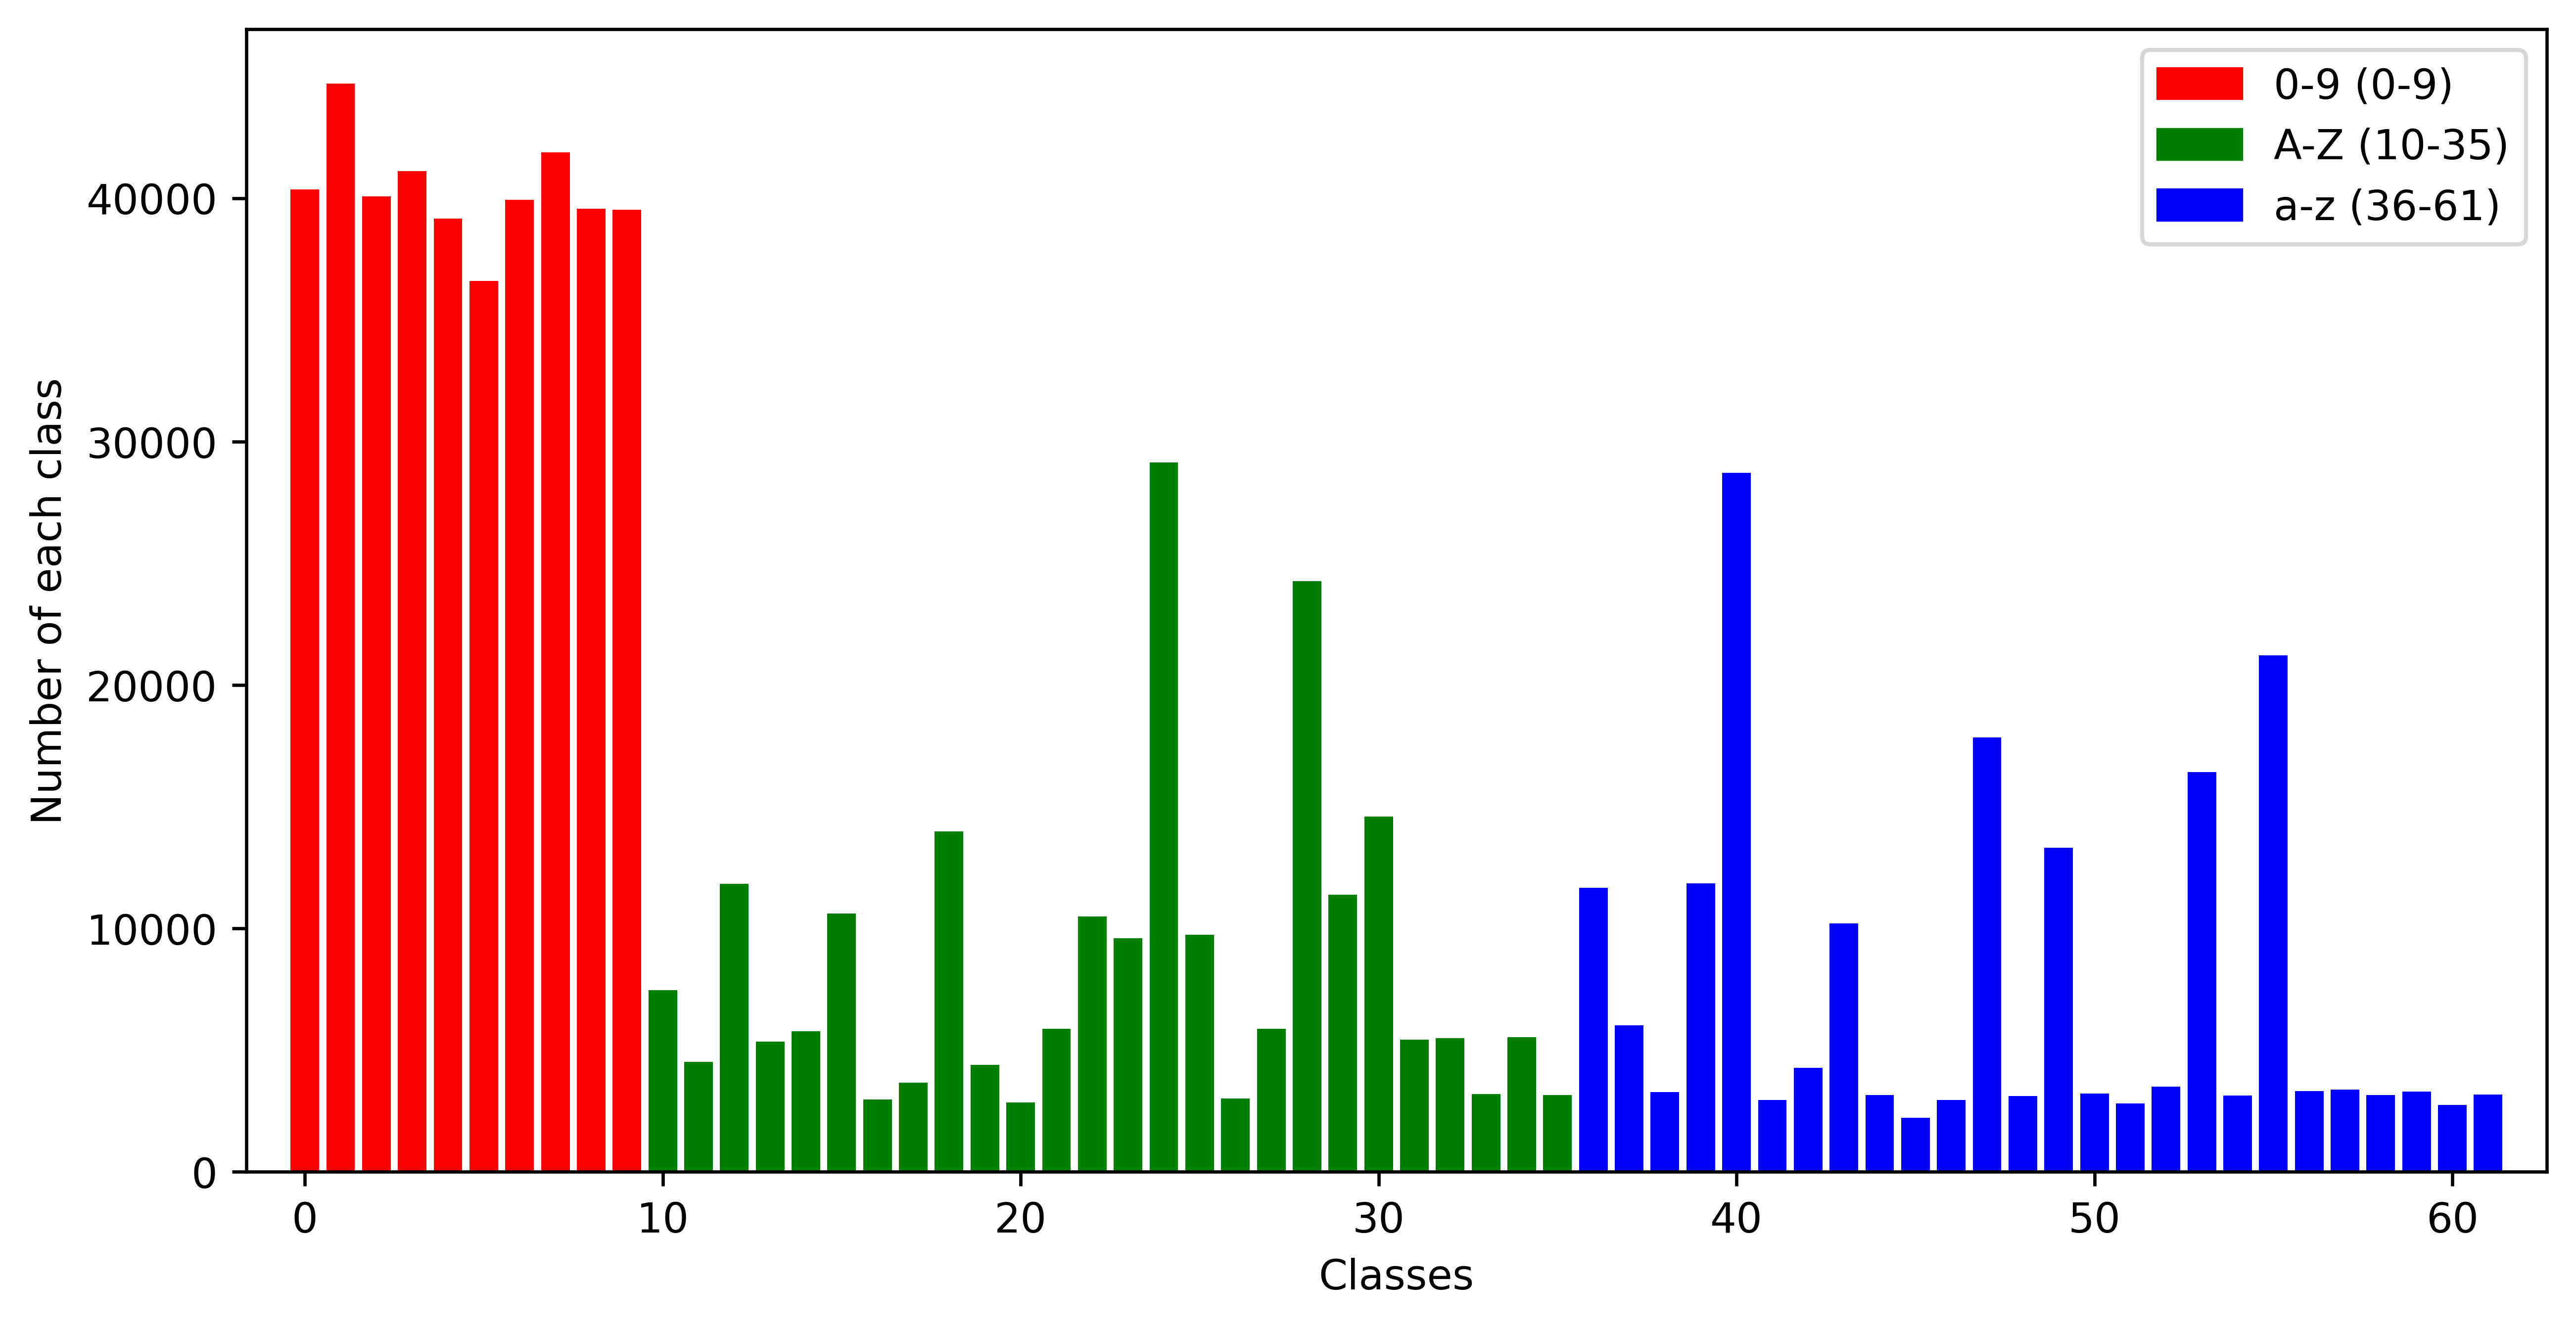
\includegraphics[scale=0.7]{images/chap5/count_all_classes.png}%
	\caption{%
تعداد داده‌های هر کلاس و نحوه نام‌گذاری در مجموعه داده
		\lr{FEMNIST}.
	}
	\label{count_all_classes}
	\centering
\end{figure}



یکی از ویژگی‌های برجسته مجموعه داده
\lr{FEMNIST}،
نحوه سازماندهی داده‌ها است. این مجموعه داده بر اساس کاربران مختلف تقسیم‌بندی شده است، به طوری که هر کاربر دارای مجموعه‌ای از داده‌های دست‌نوشته خود است. این سازماندهی امکان آزمایش و ارزیابی روش‌های یادگیری فدرال را فراهم می‌کند، زیرا در یادگیری فدرال داده‌ها به صورت محلی بر روی دستگاه‌های کاربران، نگه‌داری می‌شوند و مدل‌ها بر روی این داده‌ها آموزش می‌بینند. این ویژگی به محققان اجازه می‌دهد تا سناریوهای واقعی‌تری از یادگیری فدرال را شبیه‌سازی و بررسی کنند.

مجموعه داده
\lr{FEMNIST}
به صورت پیش‌فرض شامل 3597 کاربر است که داده‌ها میان این کاربران توزیع شده‌اند. این توزیع نه از لحاظ تعداد تصاویر بین کاربران و نه از لحاظ پوشش‌دهی کلاس‌ها در هر کاربر، یکسان نیست. با این حال، تعداد کاربران و نحوه توزیع داده‌ها میان آنها را می‌توان به دلخواه تغییر داد.

برای بررسی حالت پیش‌فرض، می‌توان مشاهده کرد که هر کاربر چه تعداد کلاس را پوشش داده است. در شکل
\ref{clients_cover_classes}
قابل مشاهده است که هر کاربر چند کلاس را شامل می‌شود. به عنوان مثال، این شکل نشان می‌دهد که حدود 400 کاربر وجود دارند که هر کدام 58 کلاس را پوشش داده‌اند. همچنین برای بررسی تعداد تصاویری که در هر کاربر وجود دارد، می‌توان به شکل
\ref{clients_images}
توجه کرد. این شکل نشان می‌دهد که حدودا 480 کاربر وجود دارند که هر کدام 175 تصویر را شامل می‌شوند.



\begin{figure}[t]
	\centering
	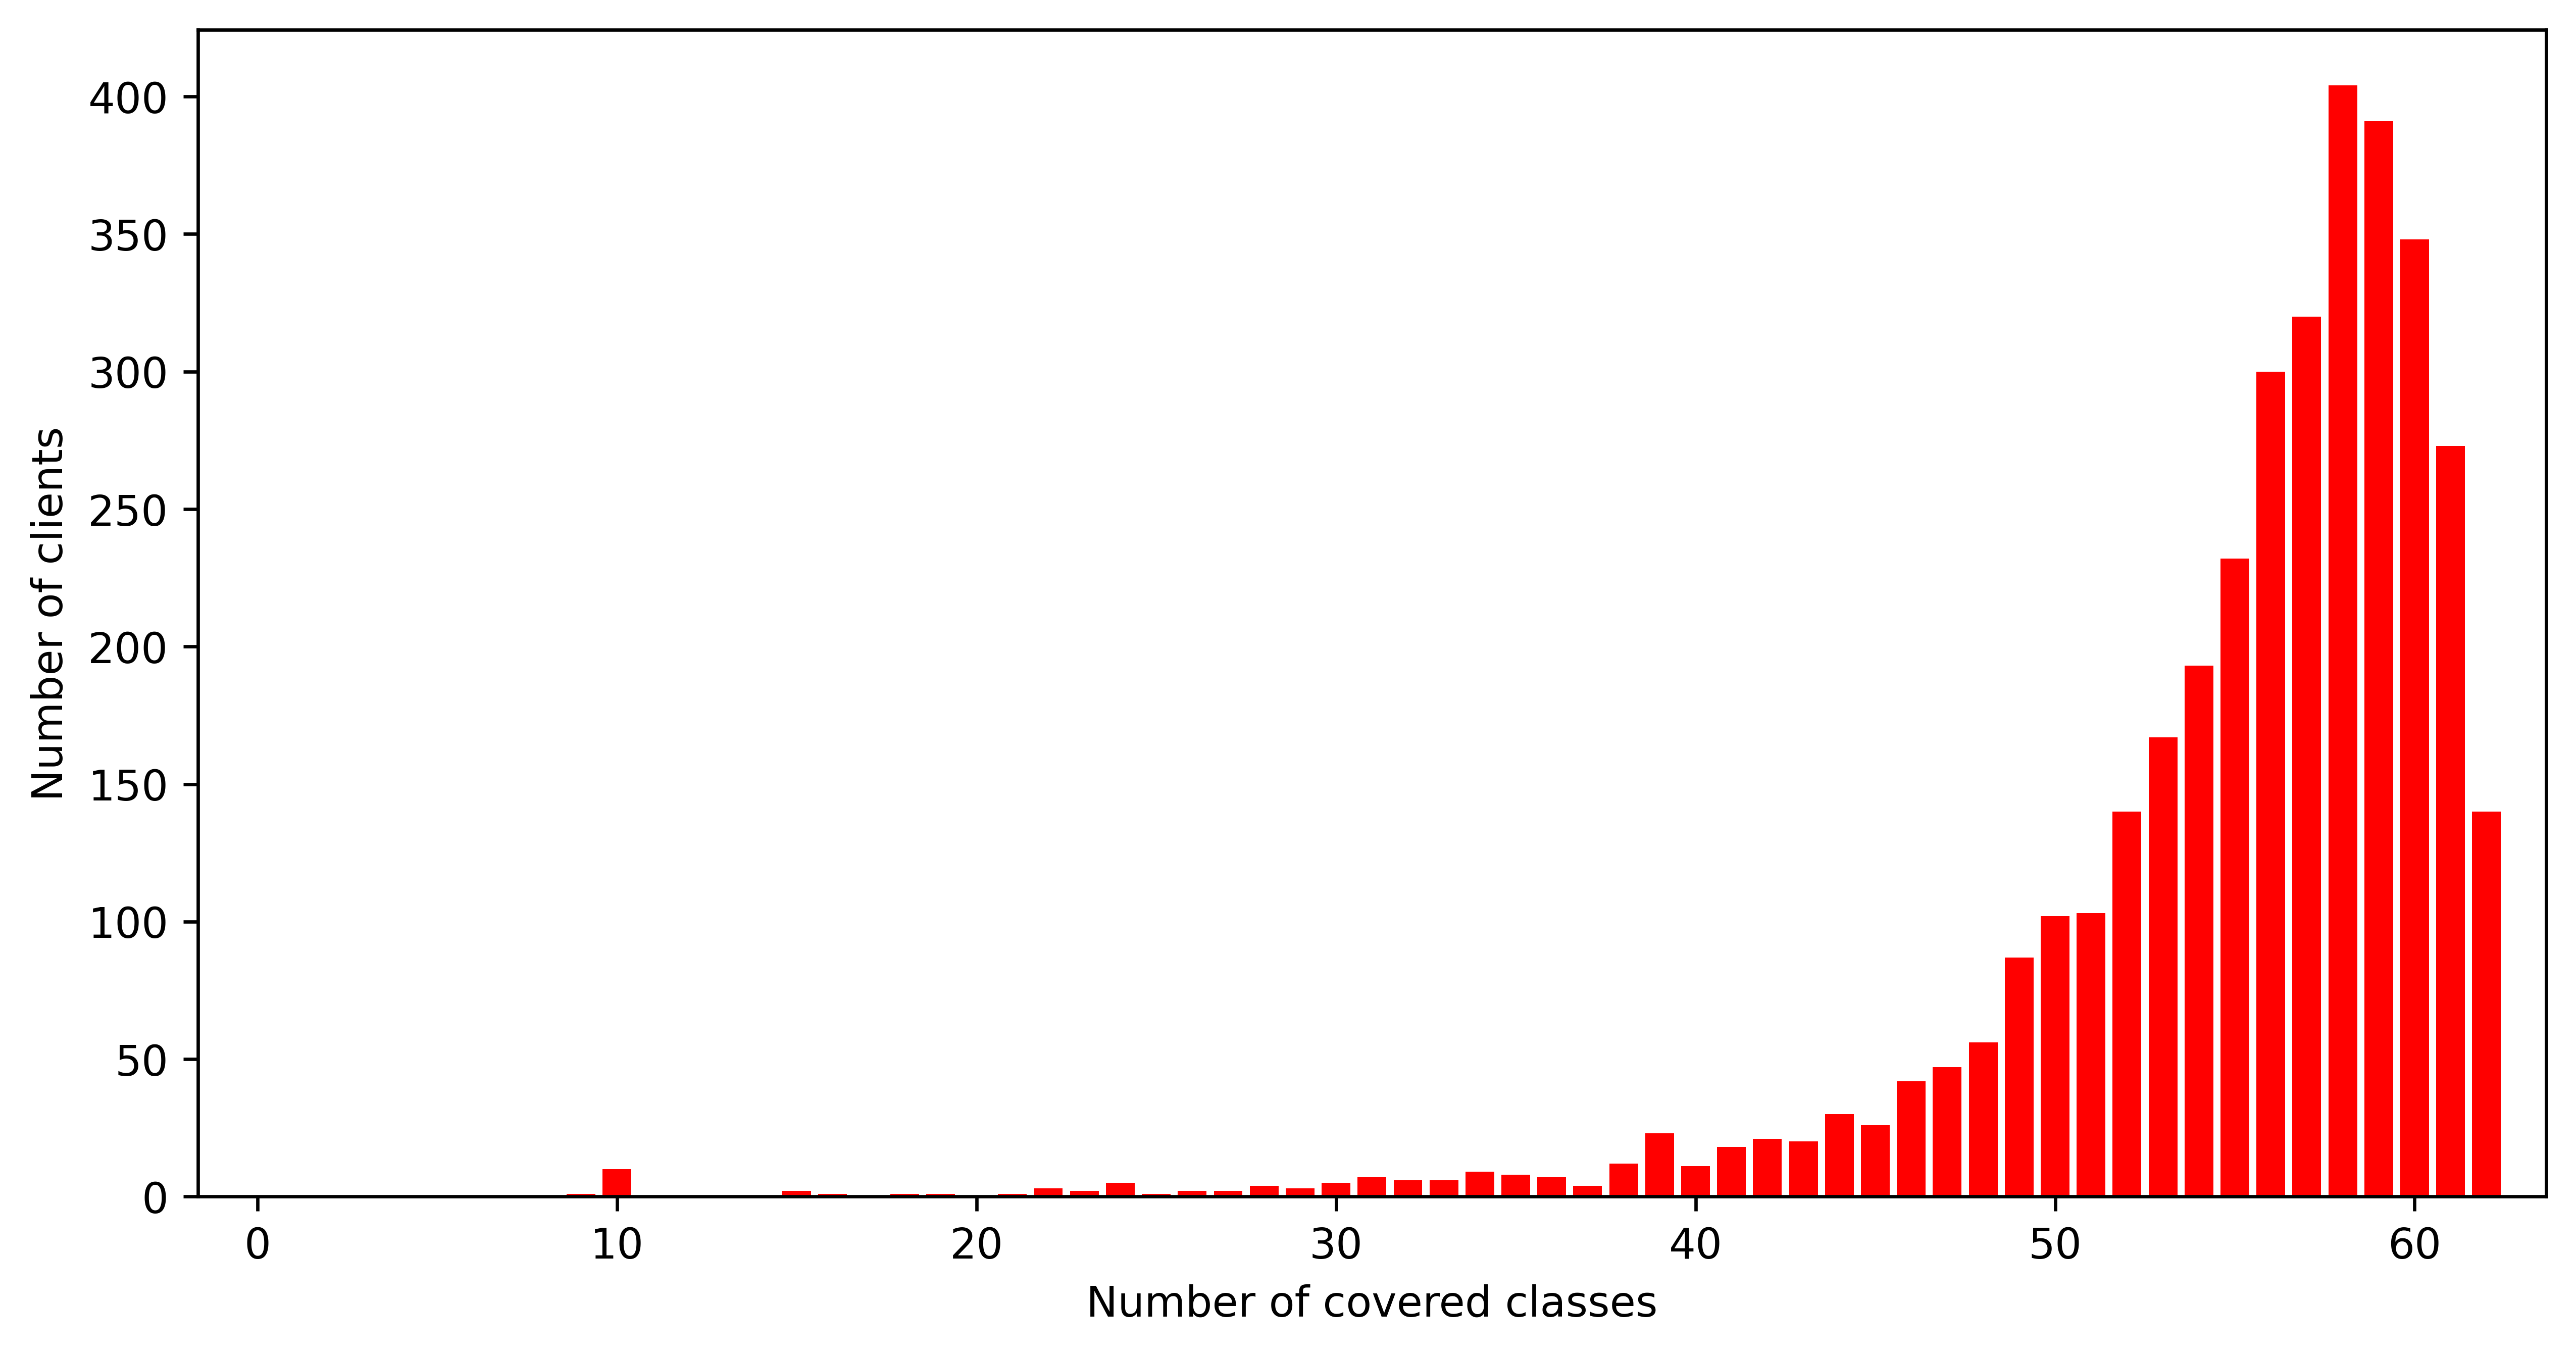
\includegraphics[scale=0.7]{images/chap5/clients_cover_classes.png}%
	\caption{%
تعداد کلاس‌های پوشش‌داده شده توسط کاربران در مجموعه داده
		\lr{FEMNIST}.
	}
	\label{clients_cover_classes}
	\centering
\end{figure}


\begin{figure}[t!]
	\centering
	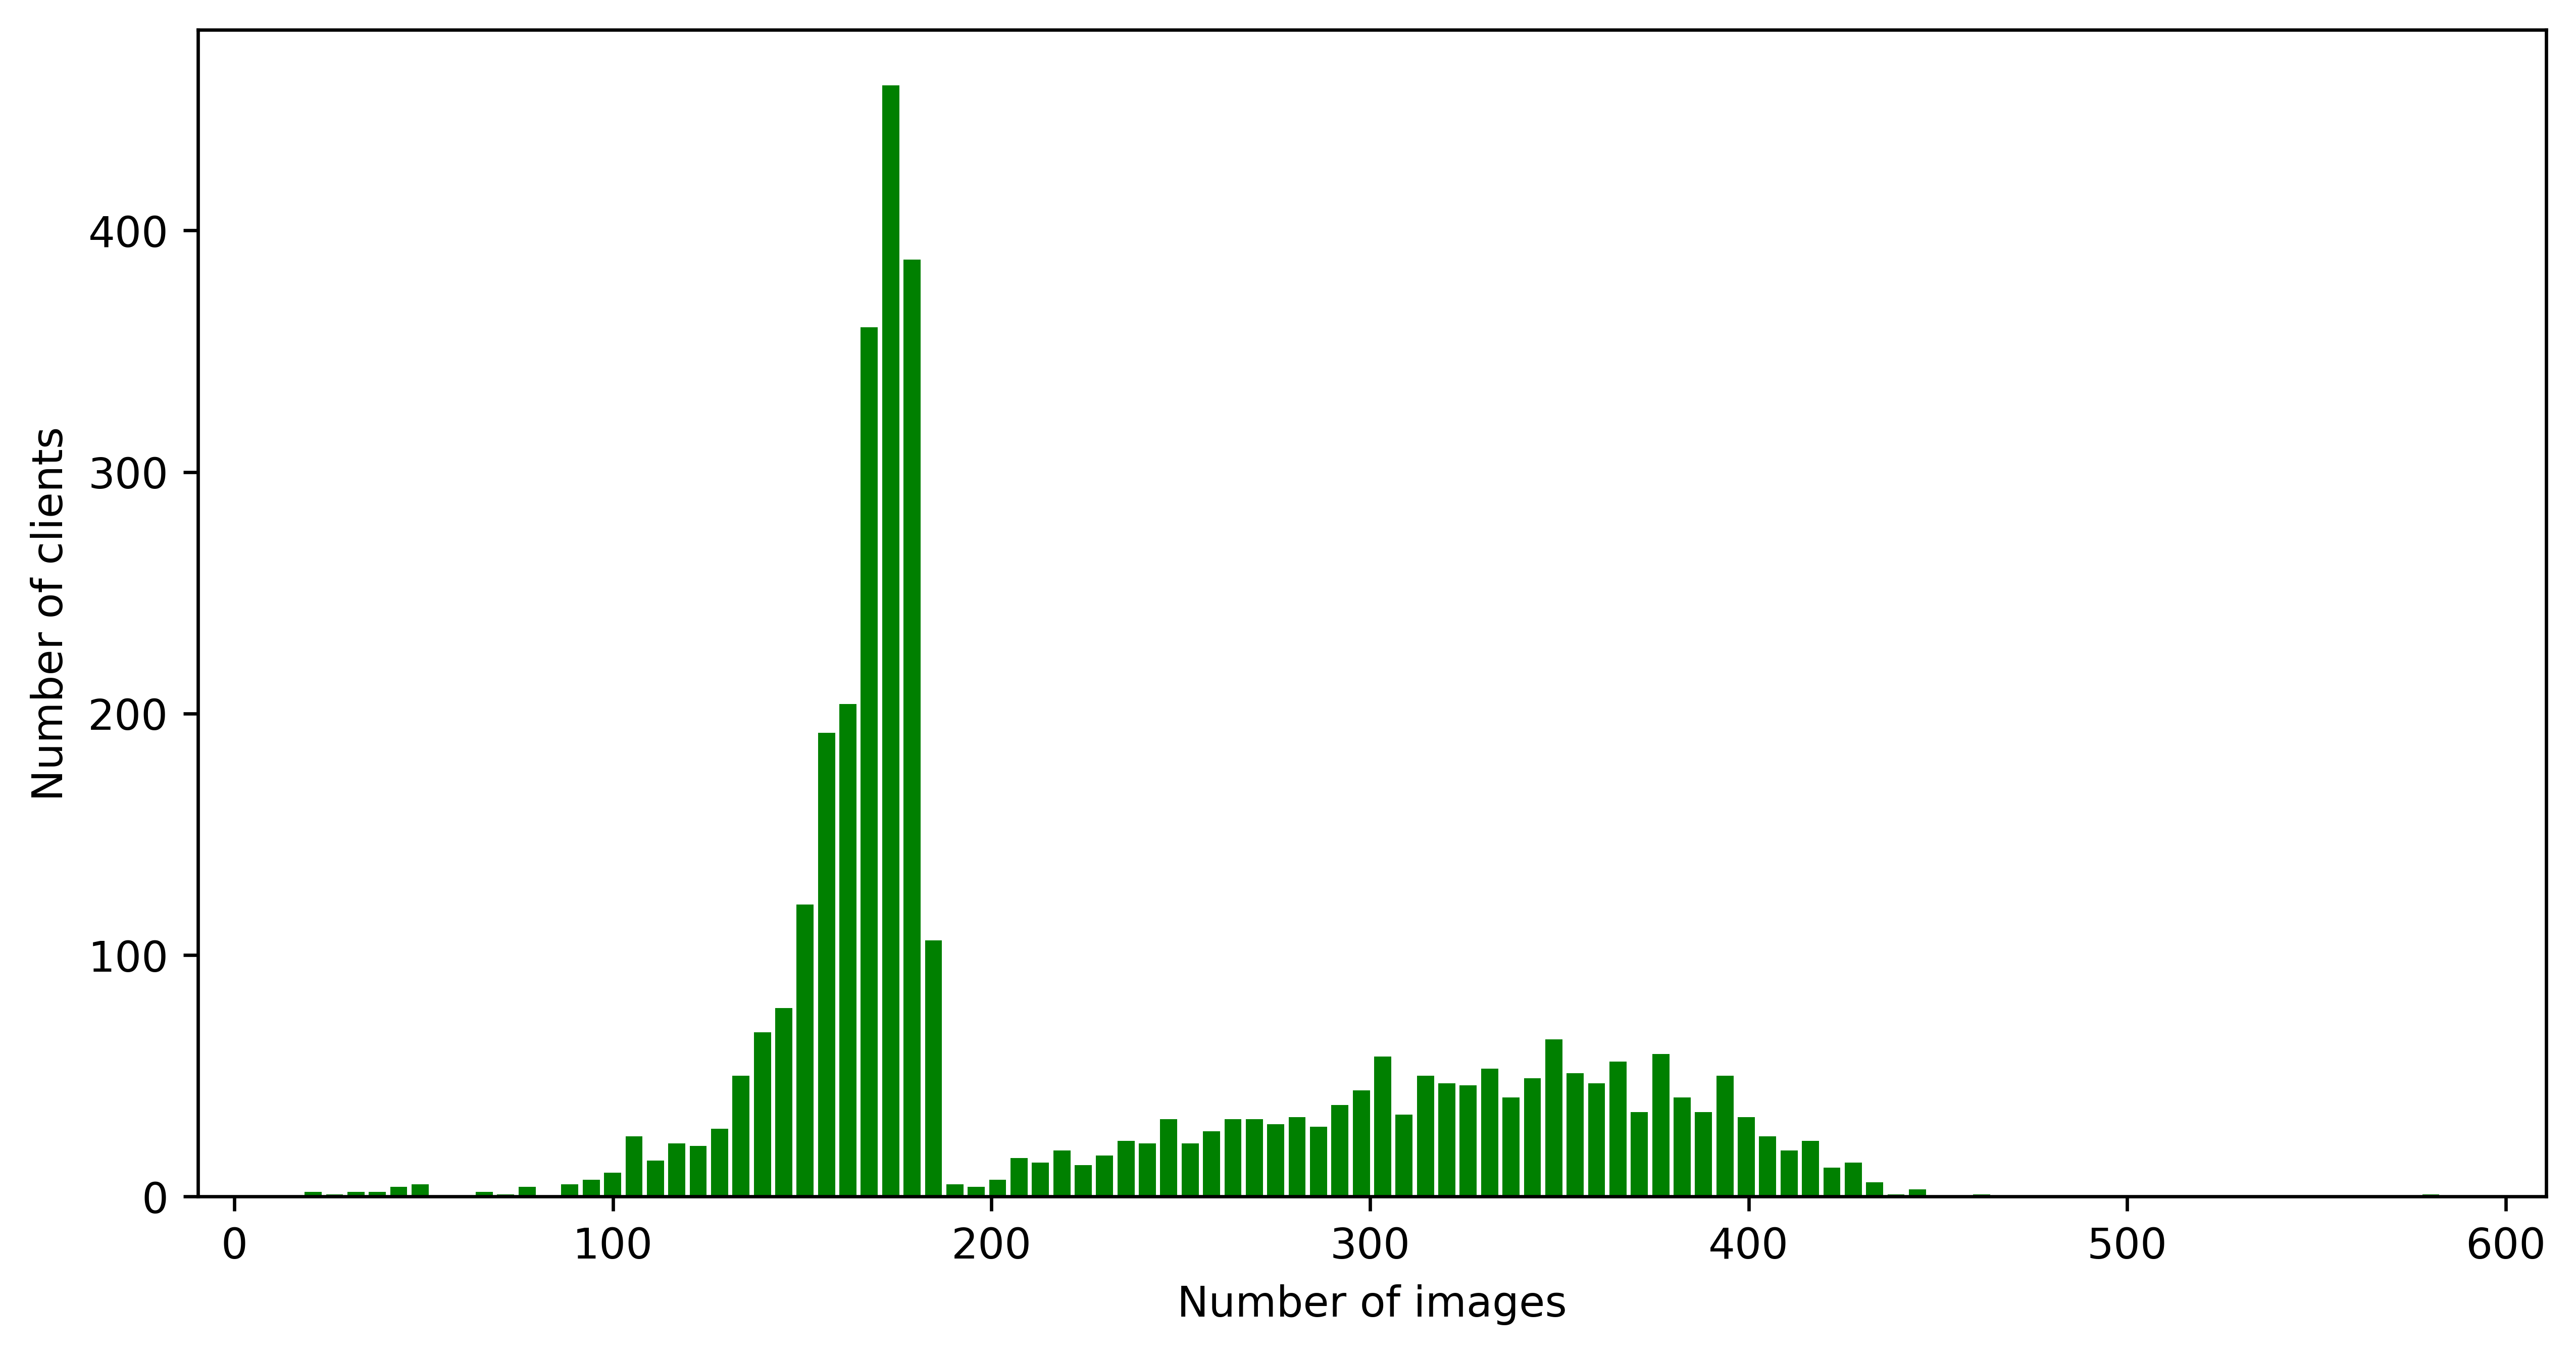
\includegraphics[scale=0.7]{images/chap5/clients_images.png}%
	\caption{%
		تعداد تصاویر هر یک از کاربران در مجموعه داده
		\lr{FEMNIST}.
	}
	\label{clients_images}
	\centering
\end{figure}



تصاویر در مجموعه داده
\lr{FEMNIST}
به صورت سیاه و سفید و با اندازه
28$\times$28
پیکسل هستند. هر تصویر نمایانگر یک کاراکتر دست‌نوشته است. این تصاویر از مجموعه داده
\lr{NIST}
استخراج شده‌اند و به صورت مناسبی برای کاربردهای یادگیری فدرال سازماندهی شده‌اند. در حقیقت این تصاویر شامل نویسه‌های مختلف از کاربران مختلف است که تنوع در سبک نوشتن و کیفیت دست‌نوشته‌ها را افزایش می‌دهد.


به طور کلی، مجموعه داده
\lr{FEMNIST}
یک ابزار قدرتمند برای تحقیقات در زمینه یادگیری فدرال است. با ارائه تنوع بالای داده‌ها و سازماندهی مناسب برای سناریوهای یادگیری فدرال، این مجموعه داده به محققان کمک می‌کند تا روش‌ها و الگوریتم‌های جدید را در محیط‌های واقعی‌تر آزمایش کنند. این ویژگی‌ها باعث شده تا
\lr{FEMNIST}
به عنوان یکی از مجموعه داده‌های مرجع در این حوزه شناخته شود و در بسیاری از تحقیقات علمی و صنعتی مورد استفاده قرار گیرد.



\section{پیاده‌سازی مدل‌های شبکه‌عصبی}
در این بخش، دو ساختار و مدل اصلی شبکه‌های عصبی که طراحی شده‌اند، مورد بررسی قرار خواهند گرفت. این دو ساختار اصلی شامل شبکه عصبی پرسپترون چندلایه
\lr{(MLP)}%
\LTRfootnote{Multilayer Perceptron}
و شبکه عصبی پیچشی
\lr{(CNN)}%
\LTRfootnote{Convolutional Neural Network}
می‌باشند. در ادامه، هر یک از این مدل‌های طراحی شده به صورت مفصل توضیح داده خواهند شد. این توضیحات به منظور فراهم آوردن درکی جامع از نحوه عملکرد هر مدل و نقش آن‌ها در بررسی نتایج و مقایسه روش‌ها در پژوهش انجام خواهد شد. استفاده از این مدل‌ها به تحلیل و ارزیابی دقیق‌تر نتایج کمک کرده و مقایسه‌ای جامع از روش‌های مختلف را ممکن می‌سازد.

\subsection{
مدل
\lr{MLP}
}
در شبکه عصبی چندلایه تعریف شده، ابتدا لایه‌های شبکه عصبی در قالب یک ساختار ترتیبی%
\LTRfootnote{Sequential}
با استفاده از یک دیکشنری مرتب%
\LTRfootnote{OrderedDict}
تعریف می‌شوند. این ساختار ترتیب‌دار باعث می‌شود که لایه‌ها به صورت متوالی اجرا شوند و خروجی هر لایه به عنوان ورودی به لایه بعدی منتقل شود.

اولین لایه، یک لایه کاملاً متصل است که تعداد نورون‌های ورودی آن برابر با تعداد ویژگی‌های ورودی مدل به صورت تخت‌شده%
\LTRfootnote{Flatten}
و تعداد نورون‌های خروجی آن 256 است. این لایه تمام اتصالات ممکن بین نورون‌های ورودی و خروجی را دارد. پس از این لایه، یک تابع فعال‌سازی 
\lr{ReLU}
قرار دارد که وظیفه آن این است که تمامی مقادیر منفی خروجی را به صفر تبدیل کند و مقادیر مثبت را بدون تغییر نگه دارد.

لایه دوم، یک لایه کاملاً متصل دیگر است که 256 نورون ورودی و 128 نورون خروجی دارد. پس از این لایه نیز یک تابع فعال‌سازی
\lr{ReLU}
قرار دارد که مشابه تابع فعال‌ساز قبلی عمل می‌کند. سومین لایه نیز دقیقا مشابه لایه دوم است با این تفاوت که 128 نورون به عنوان ورودی و 64 نورون به عنوان خروجی دارد و در ادامه آن هم تابع فعال‌سازی
\lr{ReLU}
وجود دارد.

چهارمین و آخرین لایه، یک لایه کاملاً متصل است که 64 نورون ورودی و تعداد نورون‌های خروجی آن برابر با تعداد کلاس‌های موجود در مسئله طبقه‌بندی است. این لایه خروجی‌های نهایی شبکه را تولید می‌کند که نشان‌دهنده میزان تعلق هر ورودی به هر یک از کلاس‌ها است.

در نهایت، یک لایه 
\lr{Softmax}
اضافه شده است که وظیفه آن تبدیل خروجی‌های نهایی شبکه به توزیع احتمالاتی است. این لایه کمک می‌کند تا بتوان احتمال تعلق هر ورودی به هر کلاس را به صورت عددی بین صفر و یک بدست آورد که جمع کل این احتمالات برای همه کلاس‌ها برابر با یک خواهد بود. این توزیع احتمالاتی برای انجام پیش‌بینی‌های نهایی مورد استفاده قرار می‌گیرد. در پایان می‌توانید ساختار این مدل را در شکل
\ref{mlp}
مشاهده نمایید.

\begin{figure}[b!]
	\centering
	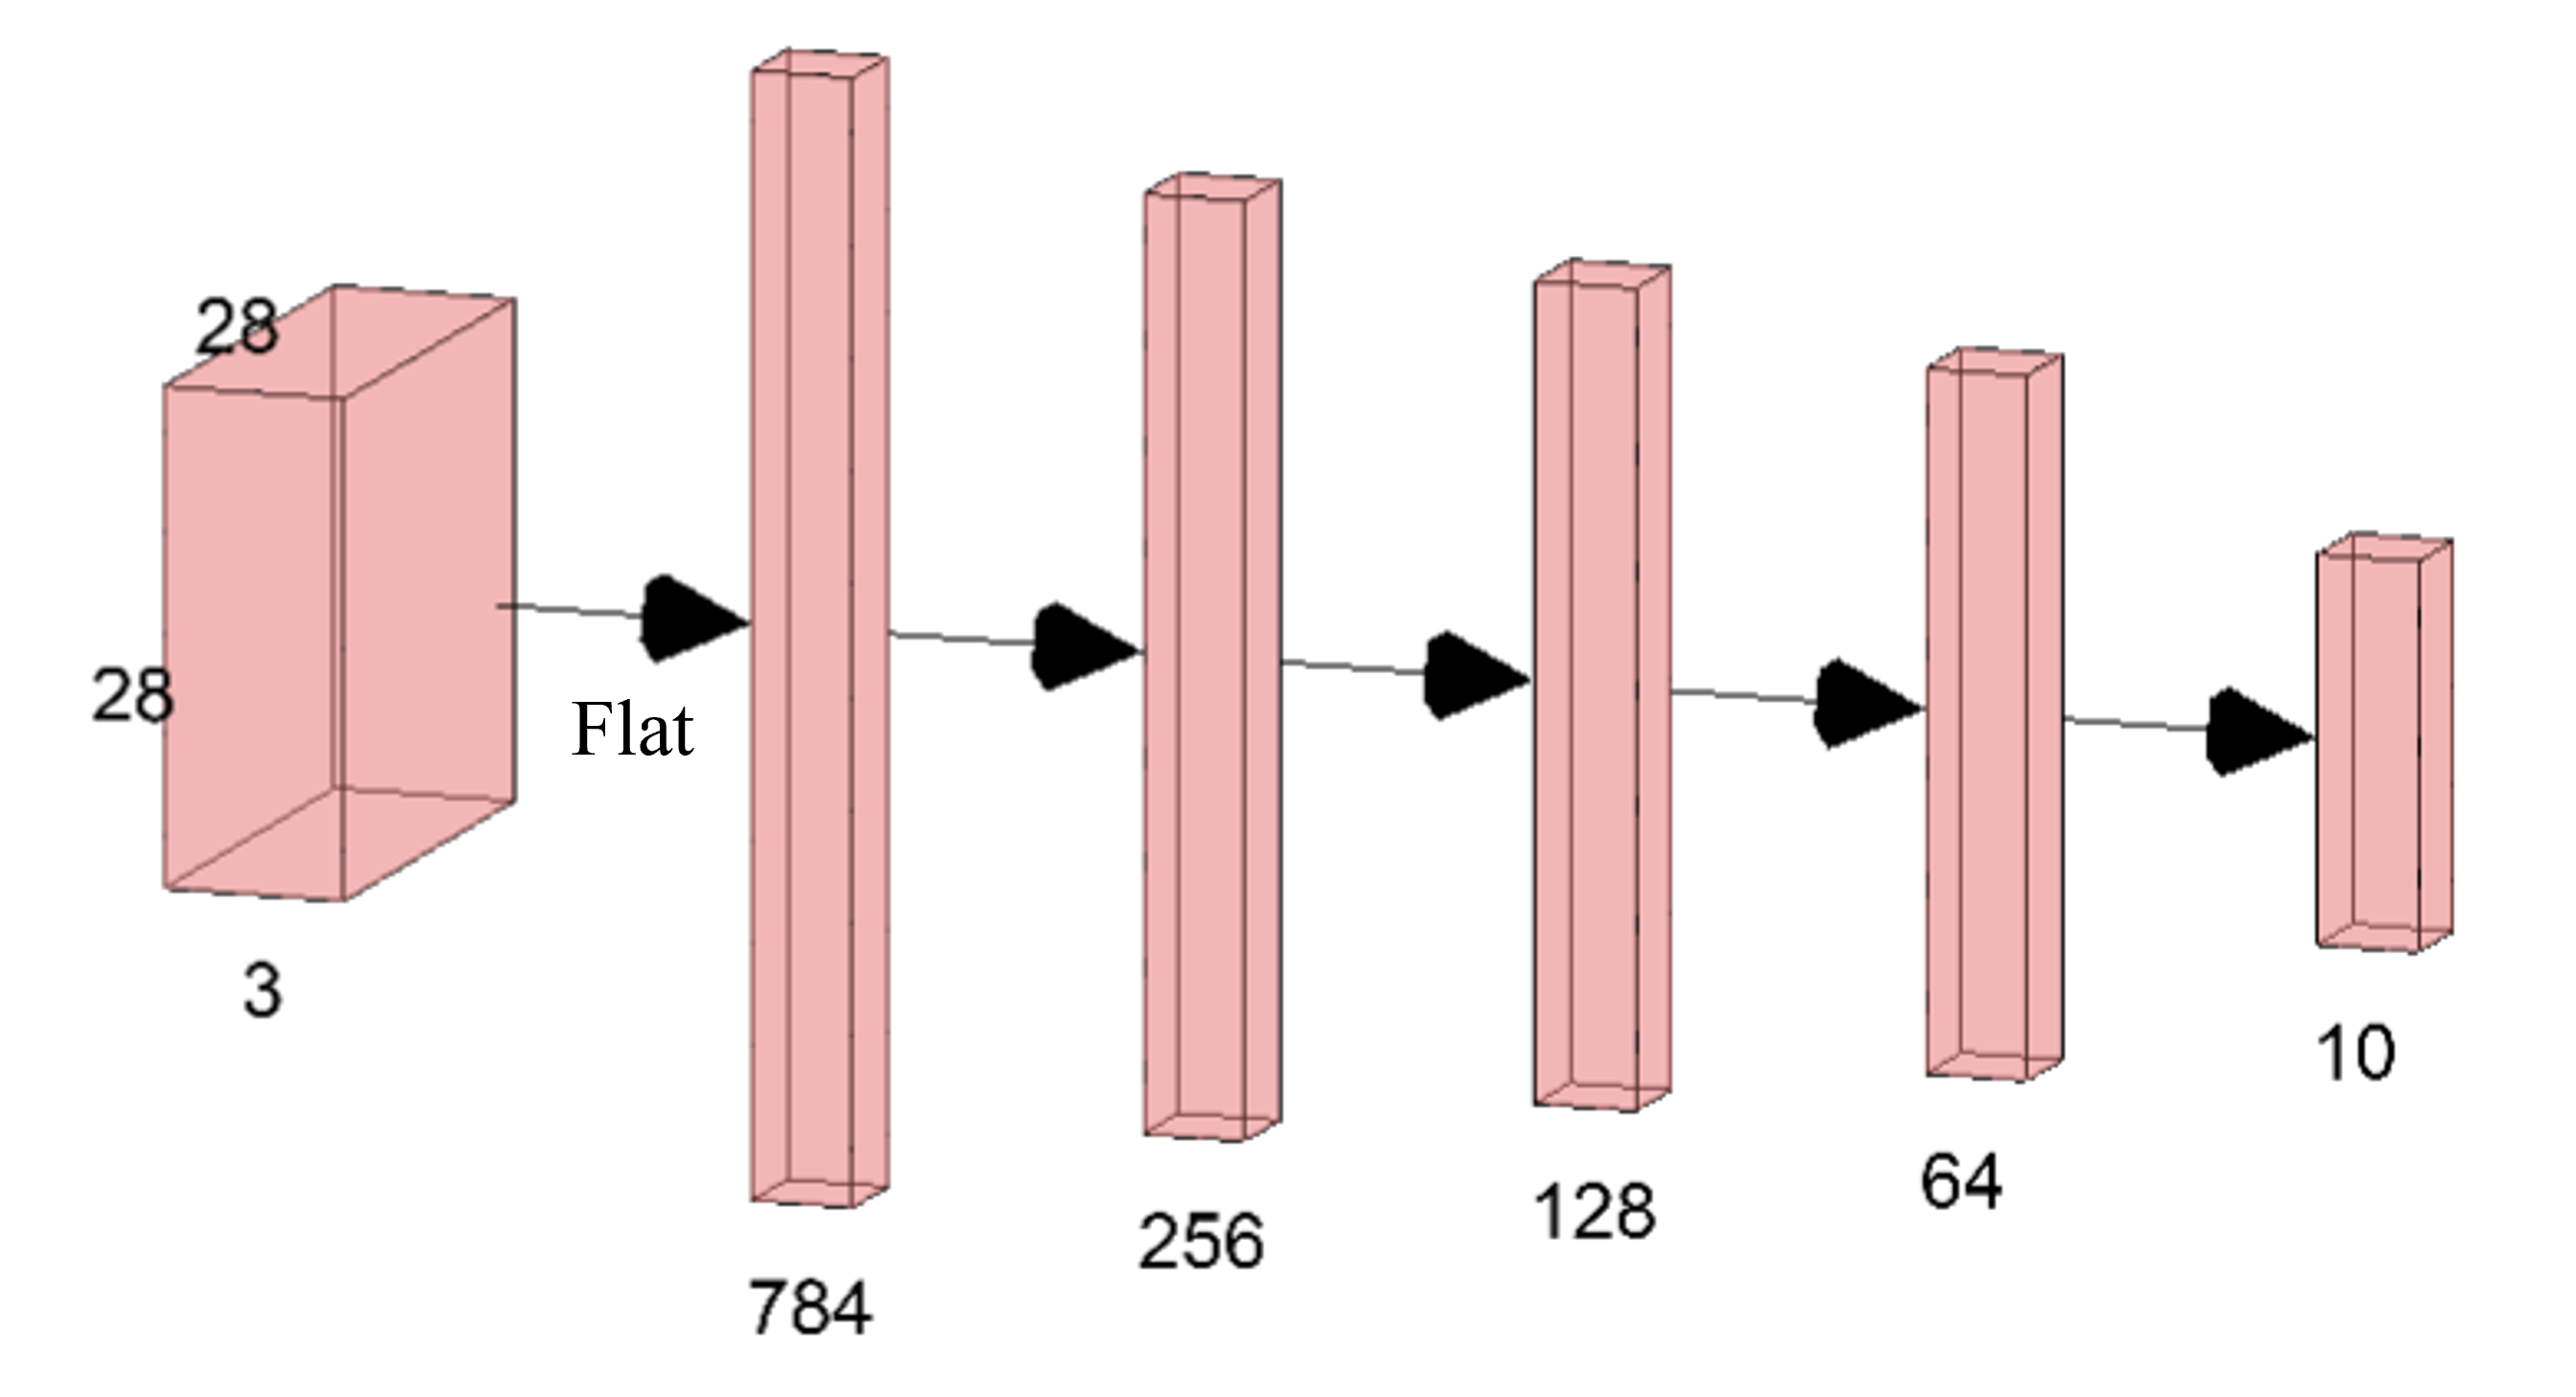
\includegraphics[scale=0.7]{images/chap5/mlp.png}%
	\caption{
		ساختار مدل 
		\lr{MLP}
	}
	\label{mlp}
	\centering
\end{figure}



\subsection{
	مدل
	\lr{CNN}
}
در شبکه عصبی پیچشی، ابتدا یک بلوک ترتیبی شامل لایه‌های مختلف به کمک دیکشنری مرتب تعریف شده است. این لایه‌ها به ترتیب وظایف مختلفی در استخراج ویژگی‌ها و انجام طبقه‌بندی نهایی دارند.

اولین لایه، یک لایه پیچشی تعریف شده است که تعداد کانال‌های ورودی تصویر را به 32 کانال خروجی تبدیل می‌کند. این لایه از یک کرنل ‎پیچشی با اندازه
3$\times$3
استفاده می‌کند. این لایه وظیفه دارد تا ویژگی‌های ابتدایی تصویر ورودی را استخراج کند. پس از این لایه، یک تابع فعال‌سازی 
\lr{ReLU}
قرار دارد که مقادیر منفی را به صفر تبدیل کرده و مقادیر مثبت را بدون تغییر نگه می‌دارد که این کار باعث ایجاد غیرخطی‌ شدن شبکه می‌شود.

سپس یک لایه تجمیع حداکثر%
\LTRfootnote{Max Pooling}
قرار دارد که اندازه فضای ویژگی‌های خروجی را کاهش می‌دهد و به کم کردن تعداد پارامترها و افزایش کارایی مدل کمک می‌کند. این لایه با انتخاب حداکثر مقدار در هر ناحیه کوچک
2$\times$2،
منجر به کاهش ابعاد تصاویر خواهد شد.

در ادامه، یک لایه پیچشی دیگر قرار دارد که تعداد کانال‌های خروجی را به 64 کانال افزایش می‌دهد. این لایه نیز از یک کرنل پیچشی با اندازه
3$\times$3
استفاده می‌کند و وظیفه استخراج ویژگی‌های پیچیده‌تر را بر عهده دارد. پس از این لایه نیز یک تابع فعال‌سازی
\lr{ReLU}
قرار دارد که مشابه قبل عمل می‌کند.

سپس یک لایه تجمیع حداکثر دیگر قرار دارد که اندازه فضای ویژگی‌های خروجی را مجدداً کاهش می‌دهد. این لایه نیز با انتخاب حداکثر مقدار در هر ناحیه کوچک
2$\times$2،
به کاهش ابعاد تصاویر کمک می‌کند.

پس از این لایه‌ها، یک لایه تخت‌کننده قرار دارد که ویژگی‌های چند بعدی خروجی را به یک بردار یک بعدی تبدیل می‌کند. این کار برای آماده‌سازی داده‌ها جهت ورود به لایه‌های کاملاً متصل انجام می‌شود.

در مرحله بعد، یک لایه کاملاً متصل قرار دارد که بردار ویژگی‌ها را به یک بردار با 100 نورون تبدیل می‌کند. این لایه تمام اتصالات ممکن بین نورون‌های ورودی و خروجی را دارد. پس از این لایه، یک تابع فعال‌سازی
\lr{ReLU}
وجود دارد که مشابه توابع فعال‌سازی قبلی عمل می‌کند و غیرخطی‌بودن را به شبکه اضافه می‌کند.

در پایان، یک لایه کاملاً متصل دیگر قرار دارد که بردار ویژگی‌ها را به یک بردار جدید با تعداد نورون‌هایی برابر با تعداد کلاس‌ها تبدیل می‌کند. این لایه، خروجی نهایی شبکه را تولید می‌کند که نشان می‌دهد هر ورودی به چه میزان به هر یک از کلاس‌ها تعلق دارد.

در انتها، یک لایه
\lr{Softmax} 
قرار داده شده که خروجی‌های نهایی شبکه را به توزیع احتمالاتی تبدیل می‌کند. این لایه باعث می‌شود که احتمال تعلق هر ورودی به هر کلاس به صورت عددی بین صفر و یک محاسبه شود، به طوری که مجموع این احتمالات برای همه کلاس‌ها برابر با یک باشد. این توزیع احتمالاتی در انتها برای انجام پیش‌بینی‌های نهایی به کار می‌رود. در پایان جهت درک بهتر می‌توانید ساختار این مدل را در شکل
\ref{cnn}
مشاهده نمایید.


\begin{figure}[t]
	\centering
	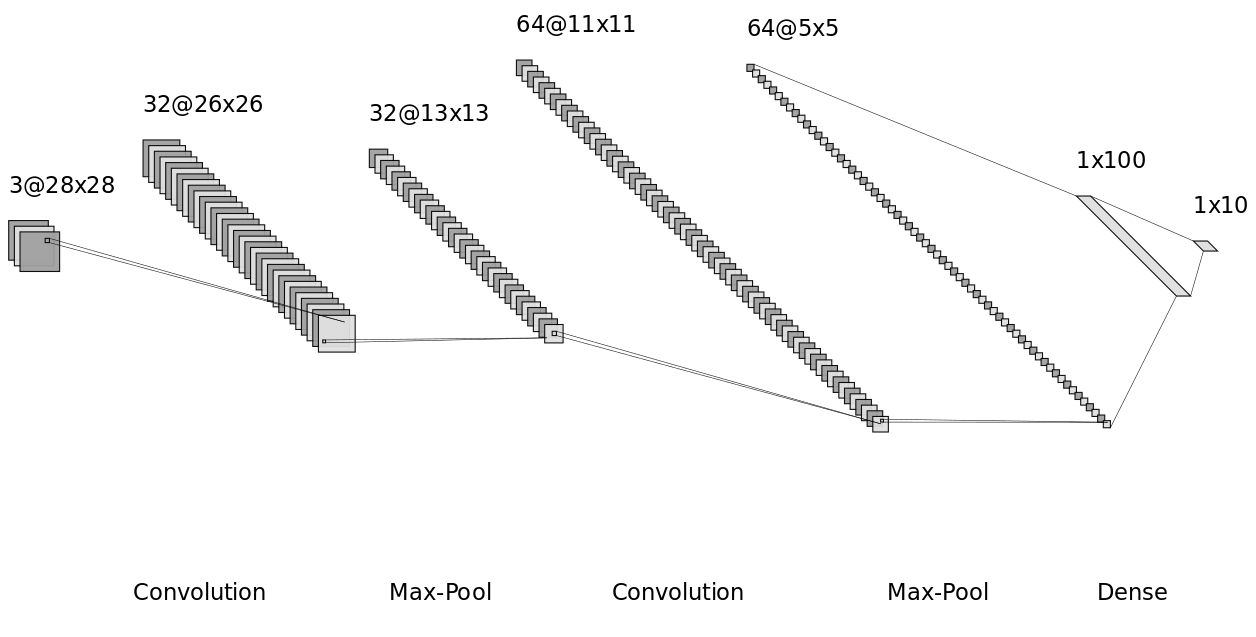
\includegraphics[scale=0.47]{images/chap5/cnn.png}%
	\caption{
		ساختار مدل 
		\lr{CNN}
	}
	\label{cnn}
	\centering
\end{figure}




\section{بررسی نتایج}
تست

\subsection{
\lr{CIFAR-10}
}
تست

با توجه به نتیجه
\ref{cifar10_r015_acc2}


\begin{figure}[t]
	\centering
	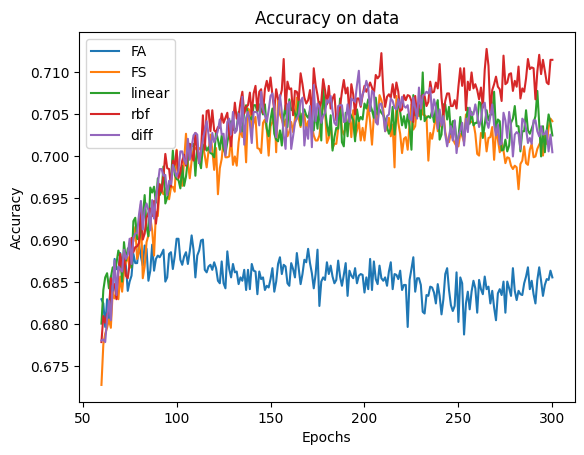
\includegraphics[scale=0.7]{images/chap5/cifar10_r015_acc2.png}%
	\caption{
		تست
		\lr{CIFAR-10}
	}
	\label{cifar10_r015_acc2}
	\centering
\end{figure}




\subsection{
	\lr{CINIC-10}
}
تست

با توجه به نتیجه
\ref{mylabel1}


\begin{figure}[t]
	\centering
	\subfigure[کل شکل]{
		\label{mylabel1}
		\includegraphics*[width=.45\textwidth]{images/chap5/cinic10_r05_acc1.png}
	}
	\hspace{3mm}
	\subfigure[بزرگ شده بخش انتهایی]{
		\label{mylabel2}
		\includegraphics*[width=.45\textwidth]{images/chap5/cinic10_r05_acc2.png}
	}
	\caption{
		تست
		\lr{CINIC-10}
	}
	\label{mylabel}
\end{figure}




\subsection{
	\lr{FEMNIST}
}
تست



% Chapter 6
\chapter{نتیجه‌گیری و پیشنهاد‌ها}

\section{نتیجه‌گیری}

در دنیای امروزی با رشد سریع فناوری و افزایش تعداد دستگاه‌های متصل به اینترنت، نیاز به برقراری ارتباطات مؤثر و حفاظت از حریم شخصی کاربران بیش از پیش اهمیت یافته است. این مسئله منجر به توسعه روش‌های توزیع‌شده‌ای مانند یادگیری فدرال شده است. در یادگیری فدرال، داده‌ها به‌جای ارسال به یک سرور مرکزی برای پردازش، در محل خود دستگاه‌ها نگهداری می‌شوند و مدل‌ها به‌صورت محلی آموزش داده می‌شوند. سپس این مدل‌ها با یکدیگر ترکیب می‌شوند تا یک مدل سراسری به‌دست آید. این روش علاوه بر کاهش نیاز به انتقال داده‌ها، حریم شخصی کاربران را نیز بهتر حفظ می‌کند.

با این حال، یادگیری فدرال با چالش‌های متعددی مواجه است. یکی از این چالش‌ها، ناهمگنی آماری داده‌ها است. این به این معناست که داده‌های موجود در دستگاه‌های مختلف می‌توانند بسیار متفاوت و گوناگون باشند. این ناهمگنی باعث می‌شود که مدل‌های محلی نتوانند به‌طور کامل ویژگی‌های تمامی داده‌ها را یاد بگیرند و در نتیجه، مدل سراسری نیز به‌خوبی همگرا نشود. در این شرایط، رسیدن به یک مدل سراسری که عملکرد قابل قبولی داشته باشد، ممکن است با مشکل مواجه شود.

برای مقابله با این چالش، یکی از راهکارهای پیشنهادی، جابه‌جایی وزن‌های شبکه عصبی بین کاربران نهایی در طول فرآیند یادگیری است. این روش باعث می‌شود که مدل‌های محلی با داده‌های متنوع‌تری روبه‌رو شوند و در نتیجه، مدل سراسری بتواند به یک همگرایی بهتر دست یابد. به عبارت دیگر، با جابه‌جایی وزن‌ها، مدل‌ها به داده‌های بیشتری دسترسی پیدا می‌کنند که این امر به بهبود کیفیت یادگیری و همگرایی مدل کمک می‌کند.

در روش‌های متداول، جابه‌جایی وزن‌ها به‌طور تصادفی انجام می‌شود، اما در این پژوهش پیشنهاد شده است که به‌جای استفاده از روش تصادفی، این جابه‌جایی به‌صورت هوشمندانه و بر اساس معیارهای شباهت انجام شود. به این صورت که مدل‌هایی که کمترین میزان شباهت را با یکدیگر دارند، جابه‌جا شوند. این رویکرد باعث می‌شود که مدل‌ها با داده‌هایی که به‌طور کامل با آن‌ها آشنا نیستند، روبه‌رو شوند و این امر می‌تواند به بهبود همگرایی مدل سراسری منجر شود. به‌عبارت دیگر، این نوع جابه‌جایی هوشمندانه می‌تواند مدل سراسری را سریع‌تر و بهتر به همگرایی نهایی هدایت کند.

یکی دیگر از جنبه‌های این پژوهش، بررسی تأثیر جابه‌جایی وزن‌ها بر حفظ حریم شخصی کاربران است. روش‌های مرسوم جابه‌جایی، این فرآیند را به‌طور مستقیم بین کاربران نهایی انجام می‌دهند. این روش اگرچه می‌تواند به کاهش سربار شبکه کمک کند، اما ممکن است به تشدید مشکلات حریم شخصی منجر شود. در این پژوهش، پیشنهاد شده است که سرور مرکزی به عنوان واسطه در فرآیند جابه‌جایی عمل کند. با این کار، حریم شخصی کاربران بهتر حفظ می‌شود و پیاده‌سازی روش‌هایی مانند حفظ حریم شخصی تفاضلی نیز ساده‌تر خواهد شد.

باید توجه داشت که هرچند این روش بهبود قابل‌توجهی در حفظ حریم شخصی ایجاد می‌کند، اما نسبت به روش‌های جابه‌جایی وزن‌ها بدون دخالت سرور، اندکی به سربار شبکه می‌افزاید. با این حال، این سربار در مقایسه با روش‌های سنتی مانند میانگین‌گیری فدرال همچنان بسیار کمتر خواهد بود. در واقع، مزایایی که این روش در بهبود همگرایی و حفاظت از حریم شخصی به ارمغان می‌آورد، به‌خوبی افزایش جزئی سربار شبکه را نسبت به روش‌های جابه‌جایی بدون دخالت سرور جبران می‌کند و آن را به یک گزینه مطلوب و کارآمد تبدیل کرده است.

در نهایت، این پژوهش نشان می‌دهد که جابه‌جایی مدل‌های شبکه عصبی به‌صورت هوشمندانه و بر اساس معیارهای شباهت، می‌تواند فرآیند همگرایی مدل سراسری را تسریع کند. این امر به‌ویژه در شرایطی که تعداد کاربران زیاد باشد، اثرات مثبت خود را بهتر نشان می‌دهد. به بیان دیگر، هرچه تعداد کاربران بیشتر باشد، مزایای استفاده از این روش بیشتر خواهد بود و بهبود قابل توجهی در فرآیند همگرایی مشاهده می‌شود.

بنابراین، در مواردی که تعداد کاربران زیاد است و داده‌ها بسیار متفاوت و پراکنده هستند، استفاده از روش‌ جابه‌جایی وزن‌ها بر پایه شباهت می‌تواند بهبود قابل ملاحظه‌ای در کارایی و سرعت همگرایی مدل سراسری به‌همراه داشته باشد. این روش نه‌تنها از نظر فنی مؤثر است، بلکه از دیدگاه حفاظت از حریم شخصی نیز بسیار مناسب به‌نظر می‌رسد.

در نتیجه، این پژوهش اهمیت و تأثیر جابه‌جایی هوشمندانه وزن‌های شبکه‌های عصبی در یادگیری فدرال را برجسته می‌کند و راهکاری جدید برای بهبود فرآیند همگرایی و حفظ حریم شخصی کاربران ارائه می‌دهد. این رویکرد می‌تواند به‌عنوان یک راه‌حل مؤثر در مواجهه با چالش‌های موجود در یادگیری فدرال مورد استفاده قرار گیرد.



\section{پیشنهادها}
با توجه به رویکردهای بررسی‌شده در زمینه حل چالش‌های یادگیری فدرال، پیشنهادهای زیر برای ادامه این پژوهش مطرح می‌گردند:

\begin{enumerate}
	\item
	بررسی معیارهای مختلف و انتخاب کمینه شباهت
	
	در آغاز کار، یک معیار شباهت در سرور مشخص می‌شود و تمام مقایسه‌های شبکه‌های عصبی بر اساس این معیار انجام می‌گیرد. با این حال، می‌توان چند معیار را برای ارزیابی شبکه‌های عصبی مد نظر قرار داد. به عنوان نمونه، ماتریس بالا ‌مثلثی برای همه معیارها محاسبه می‌شود و در مرحله انتخاب دو مدل برای جابه‌جایی، مقدار کمینه از میان تمام معیارها برگزیده می‌شود.
	
	
	\item
	میانگین وزن‌دار بین لایه‌های مختلف
	
هنگام مقایسه دو مدل شبکه عصبی، این مقایسه به‌صورت لایه به لایه انجام شده و در نهایت میانگین تمامی لایه‌ها محاسبه می‌شود. سوالی که مطرح می‌شود این است که آیا تأثیر تمام لایه‌ها به یک اندازه است که از میانگین‌گیری با وزن یکسان استفاده می‌شود؟ در این‌جا، می‌توان اهمیت هر لایه در شبکه عصبی را تعیین کرد و سپس میانگین وزن‌دار را برای مقایسه به کار برد.
	

	\item
بررسی شباهت بین لایه‌های مختلف دو شبکه عصبی، نه فقط لایه‌های متناظر

در روش موجود، مقایسه دو شبکه عصبی تنها با بررسی لایه‌های متناظر و محاسبه معیار شباهت انجام می‌گردد. با این حال، از آن‌جا که در شبکه‌های عصبی ممکن است بین لایه‌های مختلف نیز ارتباط وجود داشته باشد، امکان مقایسه لایه‌های غیرمتناظر نیز وجود دارد. از طریق ارزیابی این لایه‌ها، می‌توان شاخصی مناسب برای تعیین شباهت کلی شبکه‌ها، استخراج کرد.
\end{enumerate}



% Appendices
\appendix
% Appendix 1
\chapter{بررسی نمودارهای خطا}

\section{
	مقایسه روش
	\lr{\texttt{\fontspec{Times New Roman} SimFedSwap}}
	با روش‌های پایه
}


\subsection{
	مجموعه داده
	\lr{MNIST}
}

\begin{figure}[h]
	\centering
	\subfigure[
	دید کلی از نتیجه
	\qquad\hspace{3mm}]{
		\label{app_result_mnist_mlp_mid}
		\includegraphics*[width=.47\textwidth]{images/chap5/result/mnist/loss_mid_mlp.png}
	}
	\hspace{1.5mm}
	\subfigure[
	بزرگ‌نمایی شده بخش اصلی					
	\qquad\hspace{5mm}]{
		\label{app_result_mnist_mlp_zoom}
		\includegraphics*[width=.47\textwidth]{images/chap5/result/mnist/loss_zoom_mlp.png}
	}
	\caption{
		مقایسه منحنی‌های خطا بر روی مجموعه داده
		\lr{MNIST}
		با استفاده از مدل
		\lr{MLP}.
	}
	\label{app_result_mnist_mlp}
\end{figure}



\begin{figure}[h]
	\centering
	\subfigure[
	دید کلی از نتیجه
	\qquad\hspace{3mm}]{
		\label{app_result_mnist_cnn_mid}
		\includegraphics*[width=.47\textwidth]{images/chap5/result/mnist/loss_mid_cnn.png}
	}
	\hspace{1.5mm}
	\subfigure[
	بزرگ‌نمایی شده بخش اصلی					
	\qquad\hspace{5mm}]{
		\label{app_result_mnist_cnn_zoom}
		\includegraphics*[width=.47\textwidth]{images/chap5/result/mnist/loss_zoom_cnn.png}
	}
	\caption{
		مقایسه منحنی‌های خطا بر روی مجموعه داده
		\lr{MNIST}
		با استفاده از مدل
		\lr{CNN}.
	}
	\label{app_result_mnist_cnn}
\end{figure}





\FloatBarrier
\subsection{
	مجموعه داده
	\lr{CIFAR-10}
}


\begin{figure}[h]
	\centering
	\subfigure[
	دید کلی از نتیجه
	\qquad\hspace{3mm}]{
		\label{app_result_cifar10_equal_mid}
		\includegraphics*[width=.48\textwidth]{images/chap5/result/cifar10/loss_mid_equal.png}
	}
	\hspace{0.8mm}
	\subfigure[
	بزرگ‌نمایی شده بخش اصلی					
	\qquad\hspace{5mm}]{
		\label{app_result_cifar10_equal_zoom}
		\includegraphics*[width=.48\textwidth]{images/chap5/result/cifar10/loss_zoom_equal.png}
	}
	\caption{
		مقایسه منحنی‌های خطا بر روی مجموعه داده
		\lr{CIFAR-10}
		با توزیع داده یکنواخت.
	}
	\label{app_result_cifar10_equal}
\end{figure}



\begin{figure}[h]
	\centering
	\subfigure[
	دید کلی از نتیجه
	\qquad\hspace{3mm}]{
		\label{app_result_cifar10_normal_base}
		\includegraphics*[width=.48\textwidth]{images/chap5/result/cifar10/loss_base_normal.png}
	}
	\hspace{0.8mm}
	\subfigure[
	بزرگ‌نمایی شده بخش اصلی					
	\qquad\hspace{5mm}]{
		\label{app_result_cifar10_normal_zoom}
		\includegraphics*[width=.48\textwidth]{images/chap5/result/cifar10/loss_zoom_normal.png}
	}
	\caption{
		مقایسه منحنی‌های خطا بر روی مجموعه داده
		\lr{CIFAR-10}
		با توزیع داده نرمال.
	}
	\label{app_result_cifar10_normal}
\end{figure}



\FloatBarrier
\subsection{
	مجموعه داده
	\lr{CINIC-10}
}


\begin{figure}[h]
	\centering
	\subfigure[
	دید کلی از نتیجه
	\qquad\hspace{3mm}]{
		\label{app_result_cinic10_mid}
		\includegraphics*[width=.48\textwidth]{images/chap5/result/cinic10/loss_mid.png}
	}
	\hspace{0.8mm}
	\subfigure[
	بزرگ‌نمایی شده بخش اصلی					
	\qquad\hspace{5mm}]{
		\label{app_result_cinic10_zoom}
		\includegraphics*[width=.48\textwidth]{images/chap5/result/cinic10/loss_zoom.png}
	}
	\caption{
		مقایسه منحنی‌های خطا بر روی مجموعه داده
		\lr{CINIC-10}.
	}
	\label{app_result_cinic10}
\end{figure}



\FloatBarrier
\subsection{
	مجموعه داده
	\lr{FEMNIST}
}

\vspace{3mm}
\subsubsection{
	مقایسه نتایج در رویکرد کلاس‌بندی
	\lr{(FEMNISTclass)}
}\vspace{-1mm}



\begin{figure}[h]
	\centering
	\subfigure[
	دید کلی از نتیجه
	\qquad\hspace{3mm}]{
		\label{app_result_FEMNISTclass_base}
		\includegraphics*[width=.48\textwidth]{images/chap5/result/FEMNISTclass/loss_base.png}
	}
	\hspace{0.8mm}
	\subfigure[
	بزرگ‌نمایی شده بخش اصلی					
	\qquad\hspace{5mm}]{
		\label{app_result_FEMNISTclass_zoom}
		\includegraphics*[width=.48\textwidth]{images/chap5/result/FEMNISTclass/loss_zoom.png}
	}
	\caption{
		مقایسه منحنی‌های خطا بر روی مجموعه داده
		\lr{FEMNISTclass}.
	}
	\label{app_result_FEMNISTclass}
\end{figure}




\FloatBarrier
\vspace{3mm}
\subsubsection{
	مقایسه نتایج در رویکرد نویسندگان
	\lr{(FEMNISTwriter)}
}\vspace{-1mm}
تست



\section{
	مقایسه جابه‌جایی حریصانه با جابه‌جایی حداقل شباهت در روش
	\lr{\texttt{\fontspec{Times New Roman} SimFedSwap}}
}
تست


\section{
	تحلیل کاهش تعداد کاربران در هر دور و افزایش تعداد کل دورها در روش
	\lr{\texttt{\fontspec{Times New Roman} SimFedSwap}}
}
تست


% References
\renewcommand{\bibname}{مراجع}
\addcontentsline{toc}{section}{مراجع}

\bibliographystyle{unsrt-fa}
\bibliography{ref}

\addcontentsline{toc}{section}{چکیده انگلیسی}
\thispagestyle{empty}

\begin{latin}
\begin{center}

{\huge
Smart Swapping Approach Based on Neural Network Models Similarity for Enhancing Federated Learning
}

\vspace{1cm}

{\LARGE{Ali Bozorgzad}}

\vspace{0.2cm}

{\small a.bozorgzad@ec.iut.ac.ir}

\vspace{0.5cm}

September 07, 2024

\vspace{0.5cm}

Department of Electrical and Computer Engineering

\vspace{0.2cm}

Isfahan University of Technology, Isfahan 84156-83111, Iran

\vspace{0.2cm}

Degree: M.Sc. \hspace*{3cm} Language: Farsi

\vspace{1cm}

{\small\textbf{Supervisor: Dr. Amir Khorsandi (khorsandi@iut.ac.ir)}}
\end{center}
~\vfill



\noindent\textbf{Abstract}

\begin{small}
\baselineskip=0.6cm
Today, the explosion of data generated due to the rapid advancement of technology and the increasing number of devices connected to the internet, is the main reason to grow artificial intelligence and machine learning. But this makes effective communication and also user privacy protection more crucial than ever. Distributed methods like federated learning, are considered as an appropriate solution to meet these requirements. In federated learning, data remains on local devices instead of being sent to a central server, and models are trained locally. Then, these models are combined to create a comprehensive model. This approach not only reduces the need to transfer data but also paves the way for better user privacy protection. However, federated learning faces numerous challenges such as the statistical heterogeneity of data. The data on different devices vary significantly and this can prevent local models from effectively learning all data features. Thus, the global model does not converge as expected. This necessitates methods that focus on solving this problem with moderated computational efficiency, communication bandwidth and privacy preservation. This can be achieved by swapping neural network models between end users during the learning process. In this manner, local models encounter more diverse data, and so the convergence of the global model can be improved. In conventional methods, swapping is done based on a random selection strategy. But this study suggests an intelligent swapping method based on the similarity criteria. In this method, models with the least similarity are swapped to expose unfamiliar data to models and enhance the convergence of the global model. Furthermore, the impact of this method on preserving user privacy is discussed. By using a central server as an intermediary in the swapping process, it is shown that the proposed method can simplify the implementation of various privacy techniques. The simulation results demonstrate that the proposed intelligent swapping method can accelerate the convergence of the global model by approximately 1{\footnotesize \(\%\)} in scenarios with a large number of users.



\end{small}

\vspace{0.5 cm}

\noindent \textbf{Key Words}: Federated Learning, Distributed Learning, Non-IID Data, Neural Network Similarity, Statistical Heterogeneity

\end{latin}

%********************************
% Page before last: English Signatures
%********************************
\thispagestyle{empty}
\newgeometry{left=3cm,right=3cm,top=2cm}
\begin{latin}
\begin{center}

\includegraphics[height=3cm]{iut_logo.png}
\vspace{0.4cm}

{\large\textbf{Isfahan University of Technology}}\\

\vspace{0.4cm}
Department of Electrical and Computer Engineering

\vspace{2.5cm}

{\Huge
	Enhancing the Federated Learning Algorithm through Neural Networks Smart Swapping Based on Model Similarity
}

\vspace{1.5cm}

{\large
	A Thesis
	
	\vspace{.3cm}
	
	Submitted in partial fulfillment of the requirements
	
	\vspace{.3cm}
	
	for the degree of Master of Science
}

	\vspace{1.5cm}

{\Large
	\textbf{by}
	
	\vspace{.3cm}
	
	\textbf{Ali Bozorgzad}
}
\end{center}

\vfill

Evaluated and Approved by the Thesis Committee, on September 07, 2024
\vspace{0.5cm}

\begin{enumerate}
\item Amir Khorsandi, Assist. Prof (Supervisor)
\vspace{0.5cm}

%\item Poorya Parniani, Assoc. Prof. (Advisor)
%\vspace{0.5cm}
%
%\item Tahamtan Trabi, Prof. (Examiner)
%\vspace{0.5cm}

%\item Test Test, Assist. Prof (Examiner)
%\vspace{0.5cm}

\end{enumerate}

Behzad Nazari, Department Graduate Coordinator

\pagebreak
\end{latin}

%***************************
% last page: Blank
%***************************
\thispagestyle{empty}
\mbox{}

% It's finally over. Wasn't that hard, was it?

\end{document}